\documentclass[a4paper, 12pt]{report}

\usepackage[dvipsnames]{xcolor}

%%%%%%%%%%%%%%%%
% Set Variables %
%%%%%%%%%%%%%%%%

\def\useItalian{0}  % 1 = Italian, 0 = English

\def\courseName{Optimization}

\def\coursePrerequisites{Preventive learning of material related to the \textit{Linear Algebra} and \textit{Algorithms 2} course is recommended}

\def\book{\curlyquotes{Understanding and Using Linear Programming}, J. Matoušek, B. Gärtner}

\def\authorName{Simone Bianco}
\def\email{bianco.simone@outlook.it}
\def\github{https://github.com/Exyss/university-notes}
\def\linkedin{https://www.linkedin.com/in/simone-bianco}


%%%%%%%%%%%%
% Packages %
%%%%%%%%%%%%

\usepackage{../../../packages/Nyx/nyx-packages}
\usepackage{../../../packages/Nyx/nyx-styles}
\usepackage{../../../packages/Nyx/nyx-frames}
\usepackage{../../../packages/Nyx/nyx-macros}
\usepackage{../../../packages/Nyx/nyx-title}
\usepackage{../../../packages/Nyx/nyx-intro}

%%%%%%%%%%%%%%
% Title-page %
%%%%%%%%%%%%%%

\logo{../../../packages/Nyx/logo.png}

\if\useItalian1
    \institute{\curlyquotes{\hspace{0.25mm}Sapienza} Università di Roma}
    \faculty{Ingegneria dell'Informazione,\\Informatica e Statistica}
    \department{Dipartimento di Informatica}
    \ifdefined\book
        \subtitle{Appunti integrati con il libro \book}
    \fi
    \author{\textit{Autore}\\\authorName}
\else
    \institute{\curlyquotes{\hspace{0.25mm}Sapienza} University of Rome}
    \faculty{Faculty of Information Engineering,\\Informatics and Statistics}
    \department{Department of Computer Science}
    \ifdefined\book
        \subtitle{Lecture notes integrated with the book \book}
    \fi
    \author{\textit{Author}\\\authorName}
\fi


\title{\courseName}
\date{\today}

% \supervisor{Linus \textsc{Torvalds}}
% \context{Well, I was bored\ldots}

%%%%%%%%%%%%
% Document %
%%%%%%%%%%%%

\renewcommand{\B}{\mathcal{B}}
\newcommand{\calN}{\mathcal{N}}
\newcommand{\T}{\mathcal{T}}

\begin{document}
    \maketitle

    % The following style changes are valid only inside this scope 
    {
        \hypersetup{allcolors=black}
        \fancypagestyle{plain}{%
        \fancyhead{}        % clear all header fields
        \fancyfoot{}        % clear all header fields
        \fancyfoot[C]{\thepage}
        \renewcommand{\headrulewidth}{0pt}
        \renewcommand{\footrulewidth}{0pt}}

        \romantableofcontents
    }

    \introduction

    %%%%%%%%%%%%%%%%%%%%%

    \chapter{Flow networks}

    \section{Networks and flows}

    \begin{frameddefn}{Graph}
        A \textbf{graph} is a mathematical structure $G = (V,E)$, where $V$ is the set of \textbf{vertices} in $G$ and $E \subseteq V \times V$ is the set of \textbf{edges} that link two vertices in $G$.
        
        We will assume that each graph is \textit{simple}, meaning that there are no multiple edges between the same nodes and no loops (that being an edge from a vertex to itself).

        From now on, we will assume that $\abs{V(G)} = n$ and $\abs{E(G)} = m$.
    \end{frameddefn}

    A graph can be \textbf{directed} or \textbf{undirected}. In a directed graph we consider the edges $(u,v) \in E(G)$ and $(v,u) \in E(G)$ as two different edges, while in an undirected graph they represent the same edge.
    
    \textbf{Example:}
    \begin{center}
        \begin{tabular}{ccc}

            \textbf{Directed graph} & & \textbf{Undirected graph}\\
            \\
            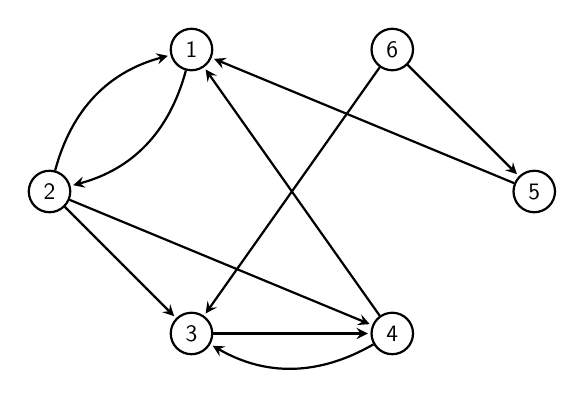
\begin{tikzpicture}[->,>=stealth,shorten >=1pt,auto,node distance=3cm,thick,main node/.style={scale=0.85,circle,draw,font=\sffamily\normalsize}]
                \node[main node] (1) {1};
                \node[main node] (2) [below left of=1] {2};
                \node[main node] (3) [below right of=2] {3};
                \node[main node] (6) [right of=1] {6};
                \node[main node] (5) [below right of=6] {5};
                \node[main node] (4) [below left of=5] {4};
    
                \path[every node/.style={font=\sffamily\small}]
                    (1) edge [bend left](2)
                    (2) edge [bend left] (1)
                    (2) edge (3)
                    (2) edge (4)
                    (3) edge (4)
                    (4) edge [bend left](3)
                    (4) edge (1)
                    (5) edge (1)
                    (6) edge (3)
                    (6) edge (5)
                    ;
            \end{tikzpicture}

            &\qquad\qquad&
            
            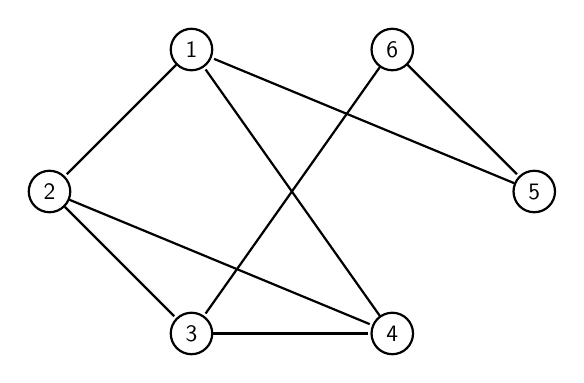
\begin{tikzpicture}[-,>=stealth,shorten >=1pt,auto,node distance=3cm,thick,main node/.style={scale=0.85,circle,draw,font=\sffamily\normalsize}]
                \node[main node] (1) {1};
                \node[main node] (2) [below left of=1] {2};
                \node[main node] (3) [below right of=2] {3};
                \node[main node] (6) [right of=1] {6};
                \node[main node] (5) [below right of=6] {5};
                \node[main node] (4) [below left of=5] {4};
    
                \path[every node/.style={font=\sffamily\small}]
                    (1) edge (2)
                    (2) edge (3)
                    (2) edge (4)
                    (3) edge (4)
                    (4) edge (1)
                    (5) edge (1)
                    (6) edge (3)
                    (6) edge (5)
                    ;
            \end{tikzpicture}
        \end{tabular}
    \end{center}

    \newpage

    \begin{frameddefn}{Network}
        A \textbf{network} is a mathematical structure $N = (G, s, t, c)$ where:
        \begin{itemize}
            \item $G = (V,E)$ is a directed graph
            \item $s$ and $t$ are two vertices of $G$ ($s,t \in V(G)$), respectively called the \textbf{source} and the \textbf{sink}
            \item $\func{c}{E(G)}{\R^+}$ is a weight function on the edges called \textbf{capacity}
            \item $(u,v) \in E(G) \implies (v,u) \in E(G)$
        \end{itemize}
    \end{frameddefn}

    \textbf{Example:}
    \begin{center}
            \begin{tikzpicture}[->,>=stealth,shorten >=1pt,auto,node distance=6.5cm,thick,main node/.style={scale=0.85,circle,draw,font=\sffamily\normalsize}]
                \node[main node, accepting] (1) {1};
                \node[main node] (2) [above right of=1] {2};
                \node[main node] (3) [below right of=1] {3};
                \node[main node, accepting] (4) [above right of=3] {4};
    
                \path[every node/.style={font=\sffamily\small}]
                    (1) edge [bend left = 40] node {5} (2)
                    (2) edge [bend left = 10, swap] node {7} (1)

                    (1) edge [bend left = 10, swap] node {4} (3)
                    (3) edge [bend left = 40] node {4} (1)

                    (2) edge [bend left = 40] node {1} (4)
                    (4) edge [bend left = 10, swap] node {3} (2)

                    (3) edge [bend left = 10, swap] node {8} (4)
                    (4) edge [bend left = 40] node {8} (3)

                    (2) edge [bend left = 20] node {5} (3)
                    (3) edge [bend left = 20] node {3} (2)
                    ;
            \end{tikzpicture}

            \textit{The numbers on the edges represent the capacities of the edges, while the nodes\\1 and 4 are chosen respectively as the source and the sink of the network}
    \end{center}

    \quad

    Essentially, a network effectively describes a \textit{water system} made up of \textit{pipes} (the edges) that can transport a maximum amount of fluid inside them (the capacity of the edges). In fact, the last property of a network defines the idea of a bi-directional \textit{flow of water} inside the pipes. In particular, we note that each pipe can have a different capacity based on the direction of the flow.



    \begin{frameddefn}{Flow}
        Given a network $N = (G, s, t, c)$, a \textbf{flow} is a weight function $\func{f}{E(G)}{\R}$ on the edges defined by the following properties:
        \begin{itemize}
            \item \textbf{Skew-symmetric}: $\forall (u,v) \in E(G) \;\; f(u,v) = -f(v,u)$, meaning that the incoming flow in an edge is the inverse of the outgoing flow in the corresponding opposite edge
            \item \textbf{Capacity bounded}: $\forall (u,v) \in E(G) \;\; f(u,v) \leq c(u,v)$, meaning that the flow can't be greater than the supported capacity
            \item \textbf{Conservation of flow}: $\forall v \in V(G) - \{s,t\}$ it holds that
            \[\sum_{\substack{(u,v) \in E(G) : \\ f(u,v) > 0}} f(u,v) = \sum_{\substack{(v,w) \in E(G) : \\ f(v,w) > 0}} f(v,w)\]
            meaning that the incoming flow in $v$ is the same as the outgoing flow from $v$
        \end{itemize}
    \end{frameddefn}

    \begin{frameddefn}{Flow value}
        Given a network $N = (G,s,t,c)$ and a flow $f$ on $N$, we define the \textbf{value of $f$}, noted by $\val(f)$, as the sum of the flow outgoing from the source $s$ or the sum of the flow incoming to the sink $t$:
        \[\val(f) := \sum_{(s,u) \in E(G)} f(s,u) = \sum_{(v,t) \in E(G)} f(v,t)\]
    \end{frameddefn}

    \textbf{Example:}
    \begin{center}
            \begin{tikzpicture}[->,>=stealth,shorten >=1pt,auto,node distance=5.75cm,thick,main node/.style={scale=0.85,circle,draw,font=\sffamily\normalsize}]
                \node[main node, accepting] (1) {1};
                \node[main node] (2) [above right of=1] {2};
                \node[main node] (3) [below right of=1] {3};
                \node[main node, accepting] (4) [above right of=3] {4};
    
                \path[every node/.style={font=\sffamily\small}]
                    (1) edge [bend left = 40] node {\color{blue} 3\color{black}, \color{red} 5} (2)
                    (2) edge [bend left = 10, swap] node {\color{blue} -3\color{black}, \color{red} 5} (1)

                    (1) edge [bend left = 10, swap] node {\color{blue} 2\color{black}, \color{red} 2} (3)
                    (3) edge [bend left = 40] node {\color{blue} -2\color{black}, \color{red} 2} (1)

                    (2) edge [bend left = 40] node {\color{blue} 3\color{black}, \color{red} 3} (4)
                    (4) edge [bend left = 10, swap] node {\color{blue} -3\color{black}, \color{red} 3} (2)

                    (3) edge [bend left = 10, swap] node {\color{blue} 2\color{black}, \color{red} 3} (4)
                    (4) edge [bend left = 40] node {\color{blue} -2\color{black}, \color{red} 3} (3)

                    (2) edge [bend left = 20] node {\color{blue} 0\color{black}, \color{red} 1} (3)
                    (3) edge [bend left = 20] node {\color{blue} 0\color{black}, \color{red} 1} (2)
                    ;
            \end{tikzpicture}

            \textit{For each edge, the numbers in blue and red respectively represent\\its flow and its capacity. The flow value of the given flow is 5.}
    \end{center}

    \newpage

    \begin{framedobs}[label=null_flow]{Nullification of flow for middle edges}
        Given a network $N = (G,s,t,c)$ and a flow $f$ defined on $G$, for each vertex different from $s$ and $t$ it holds that:
        \[\sum_{\substack{(u,v) \in E(G) : \\ f(u,v) > 0}} f(u,v) = \sum_{\substack{(v,w) \in E(G) : \\ f(v,w) > 0}} f(v,w) \iff \sum_{(u,v) \in E(G)} f(u,v) = 0\]
    \end{framedobs}

    \proofenv{

        Due to the conservation of flow and the skew-symmetric properties, for all nodes $v \neq s,t$ we know that:
        \[\sum_{\substack{(u,v) \in E(G) : \\ f(u,v) > 0}} f(u,v) =  \sum_{\substack{(v,w) \in E(G) : \\ f(v,w) > 0}} f(v,w) =  \sum_{\substack{(v,w) \in E(G) : \\ f(v,w) > 0}} -f(w,v)\]

        which is possible if only if:
        \[\sum_{\substack{(u,v) \in E(G) : \\ f(u,v) > 0}} f(u,v) = - \sum_{\substack{(v,w) \in E(G) : \\ f(v,w) > 0}} f(w,v) \iff \]
        \[\sum_{\substack{(u,v) \in E(G) : \\ f(u,v) > 0}} f(u,v) + \sum_{\substack{(v,w) \in E(G) : \\ f(v,w) > 0}} f(w,v) = 0 \]

        Again, by the skew-symmetric property we get that:
        \[\sum_{\substack{(u,v) \in E(G) : \\ f(u,v) > 0}} f(u,v) + \sum_{\substack{(v,w) \in E(G) : \\ f(v,w) > 0}} f(w,v) = 0 \iff\]
        \[\sum_{\substack{(u,v) \in E(G) : \\ f(u,v) > 0}} f(u,v) + \sum_{\substack{(w,v) \in E(G) : \\ f(w,v) < 0}} f(w,v) = 0 \]

        Then, by adding each edge incoming in $v$ that has no flow we conclude that: 
        \[\sum_{\substack{(u,v) \in E(G) : \\ f(u,v) > 0}} f(u,v) + \sum_{\substack{(w,v) \in E(G) : \\ f(w,v) < 0}} f(w,v)  + \sum_{\substack{(x,v) \in E(G) : \\ f(x,v) = 0}} f(x,v) = 0 \iff \sum_{(u,v) \in E(G)} f(u,v) = 0\]
       
    }

    \newpage

    \section{Residual graphs, flow increase and $st$-cuts}

    Consider the network shown in the last example of the previous section. 

    \begin{center}
            \begin{tikzpicture}[->,>=stealth,shorten >=1pt,auto,node distance=5.75cm,thick,main node/.style={scale=0.85,circle,draw,font=\sffamily\normalsize}]
                \node[main node, accepting] (1) {1};
                \node[main node] (2) [above right of=1] {2};
                \node[main node] (3) [below right of=1] {3};
                \node[main node, accepting] (4) [above right of=3] {4};
    
                \path[every node/.style={font=\sffamily\small}]
                    (1) edge [bend left = 40] node {\color{blue} 3\color{black}, \color{red} 5} (2)
                    (2) edge [bend left = 10, swap] node {\color{blue} -3\color{black}, \color{red} 5} (1)

                    (1) edge [bend left = 10, swap] node {\color{blue} 2\color{black}, \color{red} 2} (3)
                    (3) edge [bend left = 40] node {\color{blue} -2\color{black}, \color{red} 2} (1)

                    (2) edge [bend left = 40] node {\color{blue} 3\color{black}, \color{red} 3} (4)
                    (4) edge [bend left = 10, swap] node {\color{blue} -3\color{black}, \color{red} 3} (2)

                    (3) edge [bend left = 10, swap] node {\color{blue} 2\color{black}, \color{red} 3} (4)
                    (4) edge [bend left = 40] node {\color{blue} -2\color{black}, \color{red} 3} (3)

                    (2) edge [bend left = 20] node {\color{blue} 0\color{black}, \color{red} 1} (3)
                    (3) edge [bend left = 20] node {\color{blue} 0\color{black}, \color{red} 1} (2)
                    ;
            \end{tikzpicture}
    \end{center}

    \quad

    We notice that some \textit{pipes} aren't completely \textit{"filled up"}, meaning that their capacity could support a bigger flow. In particular, due to conservation of flow, not all pipes can be filled to the maximum capacity. In fact, we know that flow outgoing from the source must still be equal to the incoming flow of the sink.

    Thus, we can increase the flow value by 1 only by using the remaining capacities in the path $1 \to 2 \to 3 \to 4$ 
    
    \begin{center}
        \begin{tikzpicture}[->,>=stealth,shorten >=1pt,auto,node distance=5.75cm,thick,main node/.style={scale=0.85,circle,draw,font=\sffamily\normalsize}]
            \node[main node, accepting] (1) {1};
            \node[main node] (2) [above right of=1] {2};
            \node[main node] (3) [below right of=1] {3};
            \node[main node, accepting] (4) [above right of=3] {4};

            \path[every node/.style={font=\sffamily\small}]
                (1) edge [bend left = 40] node {\color{blue} 4\color{black}, \color{red} 5} (2)
                (2) edge [bend left = 10, swap] node {\color{blue} -4\color{black}, \color{red} 5} (1)

                (1) edge [bend left = 10, swap] node {\color{blue} 2\color{black}, \color{red} 2} (3)
                (3) edge [bend left = 40] node {\color{blue} -2\color{black}, \color{red} 2} (1)

                (2) edge [bend left = 40] node {\color{blue} 3\color{black}, \color{red} 3} (4)
                (4) edge [bend left = 10, swap] node {\color{blue} -3\color{black}, \color{red} 3} (2)

                (3) edge [bend left = 10, swap] node {\color{blue} 3\color{black}, \color{red} 3} (4)
                (4) edge [bend left = 40] node {\color{blue} -3\color{black}, \color{red} 3} (3)

                (2) edge [bend left = 20] node {\color{blue} 1\color{black}, \color{red} 1} (3)
                (3) edge [bend left = 20] node {\color{blue} -1\color{black}, \color{red} 1} (2)
                ;
        \end{tikzpicture}

        \textit{The flow value of the new flow is 6.}
    \end{center}

    \begin{frameddefn}{Residual capacity}
        Given a network $N = (G,s,t,c)$ and a flow $f$ on $N$, the \textbf{residual capacity} is a weight function $\func{r}{E(G)}{\R^+}$ defined as:
        \[r(u,v) = c(u,v) - f(u,v)\]
    \end{frameddefn}

    \begin{framedobs}{}
        Given a network $N = (G,s,t,c)$ and a flow $f$ on $N$, we note that:
        \[r(u,v) + r(v,u) = c(u,v) + c(v,u)\]
    \end{framedobs}

    \begin{frameddefn}{Residual graph}
        Given a network $N = (G,s,t,c)$ and a flow $f$ on $N$, we define $R \subseteq G$ as the \textbf{residual graph} of $G$ if:
        \[(u,v) \in E(R) \iff r(u,v) > 0\]
    \end{frameddefn}
    
    \textbf{Example:}

    Consider the first graph previously shown with flow value $5$. We now add the residual capacities obtained through that flow.

    \begin{center}
        \begin{tikzpicture}[->,>=stealth,shorten >=1pt,auto,node distance=6.25cm,thick,main node/.style={scale=0.85,circle,draw,font=\sffamily\normalsize}]
            \node[main node, accepting] (1) {1};
            \node[main node] (2) [above right of=1] {2};
            \node[main node] (3) [below right of=1] {3};
            \node[main node, accepting] (4) [above right of=3] {4};

            \path[every node/.style={font=\sffamily\small}]
                (1) edge [bend left = 40] node {\color{blue} 3\color{black}, \color{red} 5\color{black}, \color{ForestGreen} 2} (2)
                (2) edge [bend left = 10, swap] node {\color{blue} -3\color{black}, \color{red} 5\color{black}, \color{ForestGreen} 8} (1)

                (1) edge [bend left = 10, swap] node {\color{blue} 2\color{black}, \color{red} 2\color{black}, \color{ForestGreen} 0} (3)
                (3) edge [bend left = 40] node {\color{blue} -2\color{black}, \color{red} 2\color{black}, \color{ForestGreen} 4} (1)

                (2) edge [bend left = 40] node {\color{blue} 3\color{black}, \color{red} 3\color{black}, \color{ForestGreen} 0} (4)
                (4) edge [bend left = 10, swap] node {\color{blue} -3\color{black}, \color{red} 3\color{black}, \color{ForestGreen} 6} (2)

                (3) edge [bend left = 10, swap] node {\color{blue} 2\color{black}, \color{red} 3\color{black}, \color{ForestGreen} 1} (4)
                (4) edge [bend left = 40] node {\color{blue} -2\color{black}, \color{red} 3\color{black}, \color{ForestGreen} 5} (3)

                (2) edge [bend left = 20] node {\color{blue} 0\color{black}, \color{red} 1\color{black}, \color{ForestGreen} 1} (3)
                (3) edge [bend left = 20] node {\color{blue} 0\color{black}, \color{red} 1\color{black}, \color{ForestGreen} 1} (2)
                ;
        \end{tikzpicture}

        \textit{For each edge, the number in green represents its residual capacity}
    \end{center}

    \newpage

    Thus, the residual graph is the following:

    \begin{center}
        \begin{tikzpicture}[->,>=stealth,shorten >=1pt,auto,node distance=5cm,thick,main node/.style={scale=0.85,circle,draw,font=\sffamily\normalsize}]
            \node[main node, accepting] (1) {1};
            \node[main node] (2) [above right of=1] {2};
            \node[main node] (3) [below right of=1] {3};
            \node[main node, accepting] (4) [above right of=3] {4};

            \path[every node/.style={font=\sffamily\small}]
                (1) edge [bend left = 40] (2)
                (2) edge [bend left = 10, swap](1)

                (3) edge [bend left = 40] (1)

                (4) edge [bend left = 10, swap] (2)

                (3) edge [bend left = 10, swap] (4)
                (4) edge [bend left = 40] (3)

                (2) edge [bend left = 20] (3)
                (3) edge [bend left = 20] (2)
                ;
        \end{tikzpicture}
    \end{center}

    \begin{framedprop}{Flow-augmenting path}
        Given a network $N = (G,s,t,c)$ and a flow $f$ on $N$, let $R \subseteq G$ be the residual graph of $G$ on $f$ and let $P$ be a direct path $s \to t$ in $R$.

        Given $\alpha := \min\limits_{(u,v) \in E(P)} r(u,v)$, we define $\func{f'}{E(G)}{R}$ as:
        \[f'(u,v) = \soe{ll}{
            f(u,v) + \alpha & \text{ if } (u,v) \in E(P) \\
            f(u,v) - \alpha & \text{ if } (v,u) \in E(P) \\
            f(u,v)& \text{ otherwise} 
        }\]

        The function $f'$ is a flow for $N$ such that $\val(f') = \val(f) + \alpha$.
    \end{framedprop}
    
    \proofenv{

        Suppose that $(u,v) \in E(P)$:
        \begin{itemize}
            \item By using the skew-symmetric property of $f$, we get that:
            \[f'(u,v) = f(u,v) + \alpha \implies -f'(u,v) = -f(u,v) - \alpha = f(v,u) - \alpha\]

            Also, since $(u,v) \in E(P)$, for $(v,u)$ we get that
            \[f'(v,u) = f(v,u) - \alpha = - f'(u,v)\]

            \item By assumption, we know that $f'(u,v) = f(u,v) + \alpha$. Thus, by definition of $\alpha$ we get that:
            \[\alpha \leq r(u,v) = c(u,v) - f(u,v) \implies\]
            \[f'(u,v) = f(u,v) + \alpha \leq f(u,v) + c(u,v) - f(u,v) = c(u,v)\]
        \end{itemize}

        If $(v,u) \in E(P)$, we can get the same result by repeating the same steps. Otherwise, the flow remains unchanged, meaning that the property is already satisfied. Thus, we conclude that $f'$ is \textit{skew-symmetric} and \textit{capacity bounded}.

        Given a vertex $x \in V(G)$, if $x \notin V(P)$ then the flows of its edges are unchanged. If $x \in V(P)$, we procede by splitting the edges in $G$ through $P$:
        \[\sum_{\substack{(u,x) \in E(G):\\f'(u,x) > 0}} f'(u,x) = \sum_{\substack{(u,x) \in E(G):\\f'(u,x) > 0,\\(u,x) \in E(P)}} f'(u,x) +  \sum_{\substack{(u,x) \in E(G):\\f'(u,x) > 0,\\(x,u) \in E(P)}} f'(u,x) =\]
        \[\sum_{\substack{(u,x) \in E(G):\\f'(u,x) > 0,\\(u,x) \in E(P)}} [f(u,x) + \alpha] + \sum_{\substack{(u,x) \in E(G):\\f'(u,x) > 0,\\(x,u) \in E(P)}} [f(u,x) - \alpha] \]

        We notice that the amount of vertices in these sums is the same, implying that each time $\alpha$ gets summed in the first sum it also gets subtracted from the other sum: 
        \[\sum_{\substack{(u,x) \in E(G):\\f'(u,x) > 0,\\(u,x) \in E(P)}} [f(u,x) + \alpha] + \sum_{\substack{(u,x) \in E(G):\\f'(u,x) > 0,\\(x,u) \in E(P)}} [f(u,x) - \alpha] =\]
        \[\sum_{\substack{(u,x) \in E(G):\\f'(u,x) > 0,\\(u,x) \in E(P)}} f(u,x) + \sum_{\substack{(u,x) \in E(G):\\f'(u,x) > 0,\\(x,u) \in E(P)}} f(u,x) = \sum_{\substack{(u,x) \in E(G):\\f'(u,x) > 0}} f(u,x)\]

        By using the same argument, we get that:
        \[\sum_{\substack{(x,w) \in E(G):\\f'(x,w) > 0}} f'(x,w) = \sum_{\substack{(x,w) \in E(G):\\f'(x,w) > 0}} f(x,w)\]

        Finally, through the the \textit{conservation of flow} of $f$, we conclude that $f'$ also satisfies such property:
        \[\sum_{\substack{(u,x) \in E(G):\\f'(u,x) > 0}} f'(u,x) = \sum_{\substack{(u,x) \in E(G):\\f'(u,x) > 0}} f(u,x) = \sum_{\substack{(x,w) \in E(G):\\f'(x,w) > 0}} f(x,w) = \sum_{\substack{(x,w) \in E(G):\\f'(x,w) > 0}} f'(x,w)\]
    }
    
    \newpage

    \begin{frameddefn}{$st-$cut}
        Given a network $N = (G,s,t,c)$ and a flow $f$ on $N$, we define a \textbf{$st$-cut of $G$} as a subset $\mathcal{U} \subseteq V(G)$ that makes a partition on $V(G)$ such that $s \in \mathcal{U}, t \notin \mathcal{U}$.

        Additionally, the vertices inside of $\mathcal{U}$ are called the \textit{s-part} of the cut, while the vertices outside of $\mathcal{U}$ are called the \textit{t-part} of the cut.
    \end{frameddefn}

    \begin{framedprop}[label=flow_cut]{Flow of an $st$-cut}
        Given a network $N = (G,s,t,c)$, a flow $f$ on $N$ and an $st$-cut $\mathcal{U} \subseteq G$, we have that:
        \[\val(f) = \sum_{\substack{(u,v) \in E(G):\\u \in \mathcal{U}, v \notin \mathcal{U}}} f(u,v)\]
    \end{framedprop}

    \proofenv{

        Consider the total sum of the flows of all the vertices in $\mathcal{U}$:
        \[\sum_{u \in \mathcal{U}} \; \sum_{(u,v) \in E(G)} f(u,v)\]

        By definition, we know that $s \in \mathcal{U}$. We can separate the flows outgoing from $s$ from the rest of the flows:
        \[\sum_{u \in \mathcal{U}} \; \sum_{(u,v) \in E(G)} f(u,v) = \sum_{(s,w) \in E(G)} f(s,w) + \sum_{u \in \mathcal{U}-\{s\}} \; \sum_{(u,v) \in E(G)} f(u,v)\]

        Due to the \nameref{null_flow}, for all vertices $u,v \neq s$ we know that the total flow is qual to 0, implying that:
        \[\sum_{(s,w) \in E(G)} f(s,w) + \sum_{u \in \mathcal{U}-\{s\}} \; \sum_{(u,v) \in E(G)} f(u,v) = \sum_{(s,w) \in E(G)} f(s,w) + 0 = \val(f)\]

        We now consider again the initial total sum. We notice that:
        \[\sum_{u \in \mathcal{U}} \; \sum_{(u,v) \in E(G)} f(u,v) = \sum_{\substack{(u,v) \in E(G):\\u \in \mathcal{U}}} f(u,v)\]

        Additionally, for any $(u,v)$ if $u,v \in \mathcal{U}$ then $f(u,v)$ cancels out with $f(v,u)$, implying that:
        \[\sum_{\substack{(u,v) \in E(G):\\u \in \mathcal{U}}} f(u,v) = \sum_{\substack{(u,v) \in E(G):\\u \in \mathcal{U}, v \notin \mathcal{U}}} f(u,v)\]

        By combining the shown equalities, we conclude the proof.

    }

    \newpage


    \begin{frameddefn}{Capacity of an $st$-cut}
        Given a network $N = (G,s,t,c)$, a flow $f$ on $N$ and an $st$-cut $\mathcal{U} \subseteq G$, we define the \textbf{capacity of an $\mathbf{st-}$ cut on $G$}, noted by $c(V(G) \backslash \mathcal{U})$, as the sum of the capacities of the edges \underline{outgoing} from \textit{s-part} to the \textit{t-part}.
        \[c(V(G) \backslash \mathcal{U}) := \sum_{\substack{(u,v) \in E(G):\\u \in \mathcal{U}, v \notin \mathcal{U}}} c(u,v)\]
    \end{frameddefn}

    \begin{framedlem}[label=upper_flow]{}
        Given a network $N = (G,s,t,c)$, the maximum value of a flow on $G$ at most the minimal capacity of an $st$-cut on $G$:
        \[\max_{f \,:\, \text{flow on $G$}}(\val(f)) \leq \min_{\mathcal{U} \,:\, st- \text{cut on $G$}}(c(V(G) \backslash \mathcal{U}))\]
    \end{framedlem}

    \proofenv{

        Let $f$ be the flow on $G$ that maximizes $\val(f)$ and let $\mathcal{U} \subseteq G$ be the $st$-cut on $G$ that minimizes capacity. By the \nameref{flow_cut} and by the \textit{capacity bounded} property of $f$, we get that:
        \[\val(f) = \sum_{\substack{(u,v) \in E(G):\\u \in \mathcal{U}, v \notin \mathcal{U}}} f(u,v)\leq \sum_{\substack{(u,v) \in E(G):\\u \in \mathcal{U}, v \notin \mathcal{U}}} c(u,v) = c(V(G) \backslash \mathcal{U})\]
    }

    \section{The Ford-Fulkerson algorithm}

    \begin{framedalgo}{The Ford-Fulkerson algorithm}
        Given a network $N = (G,s,t,c)$, we define the following algorithm:

        \quad

        \begin{algorithmic}
            \Function{FordFulkerson}{$G$}
                \State{Start with the trivial flow $f$ with all 0s}
                \While{True}
                    \State{Compute the residual graph $R \subseteq G$ on flow $f$}
                    \State{Find a path $P$ in $R$ from $s \to t$}
                    \If{$P$ does not exist}
                        \State{Return $f$}
                    \Else
                        \State{Increase $f$ through the value $\alpha$ obtained by $P$}
                    \EndIf
                \EndWhile
            \EndFunction
        \end{algorithmic}
    \end{framedalgo}
    
    We note that the \textsf{FordFulkerson}$(N)$ terminates only if the augment value eventually becomes 0, implying that there is no flow-augmenting path to be used. Thus, if the capacities defined by $c$ are all integers, the algorithm always terminates.

    Moreover, the flow-augmenting path of each iteration of \textsf{FordFulkerson}$(N)$ can be found with a simple DFS search, requiring $O(n+m)$, which is also the cost needed for computing the residual graph of each iteration. Thus, the \textbf{computational complexity} of the algorithm is $O(k(n+m))$, where $k$ is the maximum number of iterations of the while loop.

    It's easy to notice that this value $k$ \textbf{depends too much on the shape of the graph $G$}. However, due to the \textit{capacity bounded} property, in the worst case we have that $k$ equals the maximum flow value. We also notice that, technically, the cost of this algorithm is \textbf{exponential}: the number of bits required to store $k$ are $\log_2 k$, but the cost relies on $2^{\log_2 k} = k$ iterations.

    \begin{framedlem}[label=ff_flow]{}
        Given a network $N = (G,s,t,c)$, if the algorithm \textsf{FordFulkerson}$(N)$ terminates then it returns a flow $f$ such that there exists an $st$-cut $\mathcal{U} \subseteq G$ for which we have that $\val(f) = c(V(G) \backslash \mathcal{U})$
    \end{framedlem}

    \proofenv{

        Let $R$ be the residual graph of $G$ on $f = \textsf{FordFulkerson}(N)$ and let $r$ be the residual capacity function obtained through $f$. We define $\mathcal{U} \subseteq G$ as:
        \[\mathcal{U} = \{x \in V(G) \mid \exists s \to x \text{ in $G'$}\}\]

        Since the algorithm terminates when there is no path from $s \to t$, we know that $t \notin \mathcal{U}$, implying that $\mathcal{U}$ is an $st$-cut of $G$. Thus, by the \nameref{flow_cut}, we have that:
        \[\val(f) = \sum_{\substack{(x,v) \in E(G):\\ x \in \mathcal{U}, v \notin \mathcal{U}}} f(x,u)\]

        By way of contradiction, we suppose that $\exists (x,v) \in E(G') \subseteq E(G)$ such that $x \in \mathcal{U}, v \notin \mathcal{U}$. By definition of $\mathcal{U}$, we know that $s \to x$ in $G'$, so by adding $(x,v)$ to the path we get that $s \to x \to y$, which contradicts $y \notin \mathcal{U}$.
        
        Thus, such edge can't exists, implying that $\forall (x,v) \in E(G)$ such that $x \in \mathcal{U}, v \notin \mathcal{U}$ it holds that $(x,v) \notin E(G')$, which by definition of residue graph implies that:
        \[\forall (x,v) \in E(G) \text{ s.t. } x \in \mathcal{U}, v \notin \mathcal{U} \;\; f(x,v) = c(x,v)\]
        
        concluding that:
        \[\val(f) = \sum_{\substack{(x,v) \in E(G):\\ x \in \mathcal{U}, v \notin \mathcal{U}}} f(x,u) = \sum_{\substack{(x,v) \in E(G):\\ x \in \mathcal{U}, v \notin \mathcal{U}}} c(x,u) = c(V(G) \backslash \mathcal{U})\]
    }

    \subsection{The Max-flow/Min-cut theorem}

    \begin{framedthm}{Max-flow/Min-cut theorem}
        Given a network $N = (G,s,t,c)$, the maximum value of a flow on $G$ at most the minimal capacity of an $st$-cut on $G$:
        \[\max_{f \,:\, \text{flow on $G$}}(\val(f)) = \min_{\mathcal{U} \,:\, st- \text{cut on $G$}}(c(V(G) \backslash \mathcal{U}))\]
    \end{framedthm}

    \proofenv{

        By the \cref{upper_flow}, we already know that:
        \[\max_{f \,:\, \text{flow on $G$}}(\val(f)) \leq \min_{\mathcal{U} \,:\, st- \text{cut on $G$}}(c(V(G) \backslash \mathcal{U}))\]

        We now consider $f' = \mathsf{FordFulkerson}(N)$. By the \cref{ff_flow}, we know that there exists an $st$-cut $\mathcal{U'} \subseteq G$ such that $\val(f') = c(V(G) \backslash \mathcal{U'})$.

        Thus, it's easy to conclude that:
        \[\max_{f \,:\, \text{flow on $G$}}(\val(f)) \geq \val(f') = c(V(G) \backslash \mathcal{U}) \geq \min_{\mathcal{U} \,:\, st- \text{cut on $G$}}(c(V(G) \backslash \mathcal{U}))\]
    }

    \begin{framedcor}{Optimality of Ford-Fulkerson}
        The Ford-Fulkerson algorithm returns a flow with \textbf{maximum value}
    \end{framedcor}

    \section{The Edmonds-Karp algorithm}

    \begin{framedalgo}{The Edmonds-Karp algorithm}
        Given a network $N = (G,s,t,c)$, we define the following algorithm:

        \quad

        \begin{algorithmic}
            \Function{EdmondsKarp}{$N$}
                \State{Start with the trivial flow $f$ with all 0s}
                \While{True}
                    \State{Compute the residual graph $R \subseteq G$ on flow $f$}
                    \State{Find the \underline{shortest} path $P$ in $R$ from $s \to t$}
                    \If{$P$ does not exist}
                        \State{Return $f$}
                    \Else
                        \State{Increase $f$ through the value $\alpha$ obtained by $P$}
                    \EndIf
                \EndWhile
            \EndFunction
        \end{algorithmic}
    \end{framedalgo}

    \begin{framedlem}[]{}
        Given a network $N = (G,s,t,c)$, if the algorithm \textsf{EdmondsKarp}$(N)$ terminates then it returns a flow $f$ such that there exists an $st$-cut $\mathcal{U} \subseteq G$ for which we have that $\val(f) = c(V(G) \backslash \mathcal{U})$

        (\textit{proof identical to} \cref{ff_flow})
    \end{framedlem}

    \begin{framedcor}{Optimality of Edmonds-Karp}
        The Edmonds-Karp algorithm returns a flow with \textbf{maximum value}
    \end{framedcor}

    The Edmonds-Keep algorithm looks identical to the Ford-Fulkerson algorithm, except for the type of path searched at each iteration. The idea behind finding the shortest path instead of a random path is to \textbf{limit} the number of iterations made by the algorithm by making them rely on the number of nodes instead of the maximum flow value. Thus, the \textbf{computational complexity} of the algorithm effectively becomes $O(mn(n+m))$, meaning that it's not an exponential algorithm. The following statements will be necessary to justify this result.

    \newpage

    \begin{framedobs}[label=sub_short_path]{}
        Given a graph $G$ and two vertices $x,y \in V(G)$, let $P$ be the shortest path from $x \to y$. Then, for each node $z_i \in V(P)$ the path $P$ contains the shortest path $P_i$ from $x \to z_i$ 
    \end{framedobs}

    \proofenv{
        
        For each node $z_1, \ldots ,z_k \in V(P)$ ($x$ and $y$ included), let $P_i$ be the shortest path from $x \to z_i$. By way of contradiction, suppose that $P_i \not\subseteq P$.

        Given an index $i$ such that $1 \leq i \leq k$, let $P_x, P_y \subseteq P$ be the sub-paths that partition $P$ by $z_i$, meaning that $x, z_1, \ldots, z_i \in V(P_x)$ and $z_{i+1}, \ldots, z_k, y \in V(P_y)$. 

        Since by assumption $P_i$ is shorter that $P_x$, we get that the path $P_i \cup P_y$ is a path from $x \to y$ that is shorter than $P$, which is a contradiction. Thus, we conclude that for each node $z_1, \ldots ,z_k \in V(P)$ it holds that $P_i \subseteq P$.

    }

    \begin{framedprop}[label=dis_app_edges]{Disappearing and appearing edges}
        Given a network $N = (G,s,t,c)$ and the computation \textsf{EdmondsKarp}$(N)$, let:
        \begin{itemize}
            \item $f_0, \ldots, f_k$ be the series of flows computed, where $f_0$ is the trivial flow
            \item $R_0, \ldots, R_k$ be the series of residue graphs computed, where $R_0$ is obtained with flow $f_i$
            \item $P_0, \ldots, P_k$ be the series of shortest paths from $s \to t$ computed on $R_i$
        \end{itemize}

        Then, $\forall u \in V(G)$ and for each index $i = 1, \ldots, k$ it holds that:
        \[(u,v) \in E(R_i), (u,v) \notin E(R_{i+1}) \implies (u,v) \in E(P_i)\]
        and that:
        \[(u,v) \notin E(R_i), (u,v) \in E(R_{i+1}) \implies (v,u) \in E(P_i)\]
    \end{framedprop}

    \proofenv{

        If $(x,y) \in E(R_i)$ but $(x,y) \notin E(R_{i+1})$, the edge got removed by the flow-increase of path $P_i$. This can only happen only if $c(x,y) = f_{i+1}(x,y) = f_i(x,y) + \alpha_{i}$, where $\alpha_{i}$ is the flow increase obtained by $P_i$, meaning that $(x,y) \in P_i$.

        Instead, if $(x,y) \notin E(R_i)$ but $(x,y) \in E(R_{i+1})$, the edge got added by the flow-increase of path $P_{i}$. This can happen only if $f_{i}(x,y) \geq  f_{i+1}(y,x)$, which in turn can happen only if the flow of the opposite edge $(x,y)$ got increased, meaning that $(y,x) \in E(P_i)$.

    }

    \begin{framedlem}[label=mon_inc_ek]{Monotone increasing distance in Edmonds-Keep}
        Given a network $N = (G,s,t,c)$ and the computation \textsf{EdmondsKarp}$(N)$, let:
        \begin{itemize}
            \item $f_0, \ldots, f_k$ be the series of flows computed, where $f_0$ is the trivial flow
            \item $R_0, \ldots, R_k$ be the series of residue graphs computed, where $R_0$ is obtained with flow $f_i$
            \item $P_i, \ldots, P_k$ be the series of shortest paths from $s \to t$ computed, where $P_i \subseteq R_i$
        \end{itemize}

        Then, $\forall u \in V(G)$ and for each index $i = 1, \ldots, k$ it holds that:
        \[\dist_{R_i}(s,u) \leq \dist_{R_{i+1}}(s,u)\] 
    \end{framedlem}

    \proofenv{

        By way of contradiction, we assume that there exist some vertices for which the statement doesnt hold, meaning that $\exists u_1, \ldots, u_k \in V(G)$ such that $\dist_{R_i}(s,u_j) > \dist_{R_{i+1}}(s,u_j)$.

        Let $v$ be the vertex picked from $u_1, \ldots, u_k$ with minimal distance from $s$ in $R_i$, meaning that:
        \[\dist_{R_i}(s,v) = \min_{j = 1}^k \dist_{R_i}(s,u_j)\]

        Consider the shortest path $P$ in $R_{i+1}$ from $s \to v$, that being the path with length $\dist_{R_{i+1}}(s,v)$. Let $u \in V(P)$ be the vertex that precedes $v$ in $P$, meaning that $(u,v) \in E(P)$.

        Since $v$ is the vertex from $u_1, \ldots, u_k$ with the shortest distance and since $\dist_{R_{i+1}}(s,u) = \dist_{R_{i+1}}(s,v) -1$ due to it being the previous vertex of $v$ in $P$, it must hold that $u \notin \{u_1, \ldots, u_k\}$ because otherwise $u$ would be the one with the shortest distance.
        
        Thus, we get that $\dist_{R_i}(s,u) \leq \dist_{R_{i+1}}(s,u)$, which implies that:
        \[\dist_{R_i}(s,u) \leq \dist_{R_{i+1}}(s,u) = \dist_{R_{i+1}}(s,v) - 1\]

        Suppose now that $(u,v) \in E(R_i)$. Given the shortest path $P'$ in $R_ii$ from $s \to u$ can be extended with $(u,v)$, we get that $\dist_{R_ii}(s,v) \leq \dist_{R_ii}(s,u) +1$. However, this would imply that:
        \[\dist_{R_i}(s,v) \leq \dist_{R_i}(s,u) +1 \leq \dist_{R_{i+1}}(s,u) +1 \leq = \dist_{R_{i+1}}(s,v)\]
        which contradicts the initial assumption. Thus, it can't be that $(u,v) \in E(R_i)$.

        Moreover, since $(u,v) \in E(P) \subseteq E(R_{i+1})$ and $(u,v) \notin E(R_i)$, by \cref{dis_app_edges} we know that:
        \[(u,v) \notin E(R_i), (u,v) \in E(R_{i+1}) \implies (v,u) \in E(P_i)\]
        
        \newpage

        Since $P_i$ is the shortest path $s \to t$ in $R_i$ and $u,v \in V(P_i)$, by \cref{sub_short_path} we know that $P_i$ also contains the shortest paths from $s \to u$ and $s \to v$ in $R_i$. In particular, the path from $s \to u$ also contains the path $s \to v$, so $\dist_{R_i}(s,v) = \dist_{R_i}(s,u) - 1$.

        Combining this with the previous results and the initial assumption, we get that:
        \[\dist_{R_i}(s,v) = \dist_{R_i}(s,u) -1 \leq \dist_{R_{i+1}}(s,u) - 1 = \dist_{R_{i+1}}(s,v) - 2 < \dist_{R_{i}}(s,v) - 2\]
        implying that $0 < -2$, which is impossible, meaning that such vertices $u_1, \ldots, u_k$ can't exists.

    }

    \begin{framedthm}{Total iterations of Edmonds-Karp}
        The total number of iterations done by the Edmonds-Karp algorithm is $O(mn)$.

        This also implies that the algorithm always terminates.
    \end{framedthm}

    \proofenv{

        Given a network $N = (G,s,t,c)$ and the computation \textsf{EdmondsKarp}$(N)$, let:
        \begin{itemize}
            \item $f_0, \ldots, f_k$ be the series of flows computed, where $f_0$ is the trivial flow
            \item $R_0, \ldots, R_k$ be the series of residue graphs computed, where $R_0$ is obtained with flow $f_i$
            \item $P_i, \ldots, P_k$ be the series of shortest paths from $s \to t$ computed, where $P_i \subseteq R_i$
        \end{itemize}

        In the following steps, we define an edge $(u,v)$ as \textit{critical} for $R_i$ if $(u,v) \in E(R_i)$ but $(u,v) \notin E(R_{i+1})$. In particular, by \cref{dis_app_edges} we know that if an edge is critical for $R_i$ then $(u,v) \in P_i$. Furthermore, for each shortest path $P_i$ we know that there is at least one critical edge inside it, that being the edge which defines the flow augmentation value $\alpha_i$ for $P_i$.

        Given an edge $(u,v) \in E(G)$, let $\pi(1), \ldots, \pi(\ell)$ be the indexes such that $1 \leq \pi(1) < \pi(2) < \ldots < \pi(\ell) \leq k$ and such that $(u,v)$ is critical for each $\pi(i)$. By \cref{sub_short_path}, we know that for each index $i = 1, \ldots, k$ it holds that:
        \[(u,v) \in E(P_{\pi(i)}) \implies \dist_{R_{\pi(i)}}(s,v) = \dist_{R_{\pi(i)+1}}(s,u) +1\]
        meaning that $(u,v) \in E(R_{\pi(i)+1})$.
        
        If $(u,v)$ is critical for both $R_{\pi(i)}$ and $R_{\pi(j)}$ (where $i < j$, meaning that $(u,v)$ disappears both times), then there must be an index $h$ such that $\pi(i) < h < \pi(j)$ where $(u,v)$ reappears, meaning that $(u,v) \notin E(G_h)$ and $h \in E(G_{h+1})$.

        Again, by \cref{dis_app_edges}, we know that:
        \[(u,v) \notin E(G_h), h\in E(G_{h+1}) \implies (v,u) \in E(P_h) \implies \dist_{R_{h}}(s,u) = \dist_{R_{h}}(s,v) +1\]

        \newpage

        Then, since $\pi(i) < h < \pi(j)$, by the \nameref{mon_inc_ek} we know that:
        \[\dist_{R_{\pi(j)}}(s,u) \geq \dist_{R_{h}}(s,u) = \dist_{R_{h}}(s,v) +1 \geq \dist_{R_{\pi(i)}}(s,u) + 2\]

        Thus, between $R_{\pi(i)}$ and $R_{\pi(j)}$ the vertex $u$'s distance increases by at least $2$. Thus, since $u$'s final distance can be at most $n-1$, meaning that $\dist_{R_{k}}(s,u) \leq n$, starting from $0$ the distance can be increased by $2$ at most $\frac{n}{2}$ times, meaning that $\ell = \frac{n}{2}$.
        
        Since each flow-augmenting shortest path computed by the algorithm implies the existence of a a critical path and since since the number of times each edge can be critical is at most $\ell = \frac{n}{2}$, the number of paths computable is at most $m \times \frac{n}{2}$, which is in $O(mn)$.

    }

    \quad

    \section{Modelling problems as networks}
    
    Considering the previous definitions, it's easy to see that for each undirected graph we can obtain an \textbf{associated network with chosen capacities} by simply \textit{"splitting"} each undirected edge $(u,v)$ into two directed edges $(u,v), (v,u)$.

    \begin{figure}[H]
        \centering
        \begin{tabular}{ccc}
            
            \begin{tikzpicture}[-,>=stealth,shorten >=1pt,auto,node distance=3.5cm,thick,main node/.style={scale=0.85,circle,draw,font=\sffamily\normalsize}]
                \node[main node, accepting] (1) {1};
                \node[main node] (2) [above right of=1] {2};
                \node[main node] (3) [below right of=1] {3};
                \node[main node, accepting] (4) [above right of=3] {4};

                \path[every node/.style={font=\sffamily\small}]
                    (1) edge [bend left] node {5} (2)

                    (1) edge [bend right, swap] node {4} (3)

                    (2) edge [bend left] node {1} (4)

                    (3) edge [bend right, swap] node {8} (4)

                    (2) edge [] node {5} (3)
                    ;
            \end{tikzpicture}

            &\qquad\qquad&

            \begin{tikzpicture}[->,>=stealth,shorten >=1pt,auto,node distance=3.5cm,thick,main node/.style={scale=0.85,circle,draw,font=\sffamily\normalsize}]
                \node[main node, accepting] (1) {1};
                \node[main node] (2) [above right of=1] {2};
                \node[main node] (3) [below right of=1] {3};
                \node[main node, accepting] (4) [above right of=3] {4};

                \path[every node/.style={font=\sffamily\small}]
                    (1) edge [bend left = 40] node {5} (2)
                    (2) edge [bend left = 10, swap] node {5} (1)

                    (1) edge [bend left = 10, swap] node {4} (3)
                    (3) edge [bend left = 40] node {4} (1)

                    (2) edge [bend left = 40] node {1} (4)
                    (4) edge [bend left = 10, swap] node {4} (2)

                    (3) edge [bend left = 10, swap] node {8} (4)
                    (4) edge [bend left = 40] node {8} (3)

                    (2) edge [bend left = 20] node {5} (3)
                    (3) edge [bend left = 20] node {5} (2)
                    ;
            \end{tikzpicture}
        \end{tabular}
    \end{figure}

    Likewise, directed graphs also have an associated network: for each edge $(u,v)$ we add an edge $(v,u)$ (unless it already exists) with capacity set to 0.

    \begin{figure}[H]
        \centering
        \begin{tabular}{ccc}
            
            \begin{tikzpicture}[->,>=stealth,shorten >=1pt,auto,node distance=3.5cm,thick,main node/.style={scale=0.85,circle,draw,font=\sffamily\normalsize}]
                \node[main node, accepting] (1) {1};
                \node[main node] (2) [above right of=1] {2};
                \node[main node] (3) [below right of=1] {3};
                \node[main node, accepting] (4) [above right of=3] {4};

                \path[every node/.style={font=\sffamily\small}]
                    (1) edge [bend left] node {5} (2)

                    (1) edge [bend right, swap] node {4} (3)

                    (2) edge [bend left] node {1} (4)

                    (3) edge [bend right, swap] node {8} (4)

                    (2) edge [] node {5} (3)
                    ;
            \end{tikzpicture}

            &\qquad\qquad&

            \begin{tikzpicture}[->,>=stealth,shorten >=1pt,auto,node distance=3.5cm,thick,main node/.style={scale=0.85,circle,draw,font=\sffamily\normalsize}]
                \node[main node, accepting] (1) {1};
                \node[main node] (2) [above right of=1] {2};
                \node[main node] (3) [below right of=1] {3};
                \node[main node, accepting] (4) [above right of=3] {4};

                \path[every node/.style={font=\sffamily\small}]
                    (1) edge [bend left = 40] node {5} (2)
                    (2) edge [bend left = 10, swap] node {0} (1)

                    (1) edge [bend left = 10, swap] node {4} (3)
                    (3) edge [bend left = 40] node {0} (1)

                    (2) edge [bend left = 40] node {1} (4)
                    (4) edge [bend left = 10, swap] node {0} (2)

                    (3) edge [bend left = 10, swap] node {8} (4)
                    (4) edge [bend left = 40] node {0} (3)

                    (2) edge [bend left = 20] node {5} (3)
                    (3) edge [bend left = 20] node {0} (2)
                    ;
            \end{tikzpicture}
        \end{tabular}

    \end{figure}

    Since they have null capacity, these additional edges will be \textit{"ignored"} by the network, even though they are still used by it. For example, if the \textit{"real"} edge $(u,v)$ has flow $f(u,v) = k$ then we know that $f(v,u) = -k$, hence its residue will be $r(v,u) = 0 - (-k) = k$, implying that it will be available in the residue graph.

    \begin{frameddefn}{Associated network}
        Given a graph $G$ with capacities $c$, we denote with $\vec{G}$ the directed graph underlying the network $N = (\vec{G}, s, t, c)$ associated to $G$.
    \end{frameddefn}

    This natural associations can be used to prove theorems or solve problems regarding undirected graphs. In the following sections, we will see two examples of how networks can be used to model problems.

    \quad

    \subsection{Menger's theorem}

    The first example of theorem provable through networks is \textbf{Menger's theorem} which discusses the problem of \textbf{finding the maximum number of pairwise edge-disjoint paths} between two nodes in a graph.

    \begin{framedlem}[label=paths_flow]{}
        Let $G$ be graph and let $N = (\vec{G}, s, t, c)$ be the network associated to $G$ such that all edges have capacity set to 1. If $G$ has at most $k$ pairwise edge-disjoint paths $s \to t$ then the maximum value of a flow $f$ on $N$ is $k$.
    \end{framedlem}

    \proofenv{
        
        Since $G$ has at most $k$ pairwise edge-disjoint paths $s \to t$, the associated graph $\vec{G}$ will have $k$ pairwise edge-disjoint paths $s \to t$ and $k$ pairwise edge-disjoint paths $t \to s$ thanks to the edges added in the associated network.

        Then, for each path $s \to t$ in $\vec{G}$ we can set $f(u,v) = 1$ and $f(v,u) = -1$ for each edge $(u,v)$ in the path. Since each path is disjoint, sending flow to one of them doesn't influence the other paths, implying that one unit of flow can be sent on each one of the $k$ paths and thus that the maximum value of $f$ is $k$.
    }

    \begin{frameddefn}{Support of a flow}
        Given a network $N = (\vec{G},s,t,c)$ and a flow $f$ on $N$, we define the \textbf{support of $f$} as the subgraph $\vec{W} \subseteq \vec{G}$ such that:
        \[E(\vec{W}) = \{(u,v) \in E(\vec{G}) \mid f(u,v) \neq 0\}\]
    \end{frameddefn}

    \begin{framedlem}{}
        Let $G$ be a graph and let $N = (\vec{G}, s, t, c)$ be the network associated to $G$ such that all edges have capacity set to 1. If the maximum value of a flow $f$ on $N$ is $k$ then the graph $W$ associated to the support graph $\vec{W}$ of $f$ has at most $k$ pairwise edge-disjoint paths $s \to t$.
    \end{framedlem}

    \proofenv{
        
        Let $f$ be a flow on $N$ with maximum value, $\vec{W} \subseteq \vec{G}$ be the support graph of $f$ and $W$ the graph associated to $\vec{W}$. By strong induction on the number $m$ of edges in $W$, meaning that $\abs{E(W)} = m$, we show that $W$ has maximum $k$ pairwise edge-disjoint paths $s \to t$.

        If $m = 0$, then $\forall (u,v) \in E(G)$ it holds that $f(u,v) = 0$, implying that $\val{f} = 0$ and that the number of pairwise edge-disjoint paths $s \to t$ in $W$ is $0$. We now assume by strong induction that the statement holds for all graphs whose support graph has at most $m$ edges.

        Suppose now that $\abs{E(W)} = m+1$. In $\vec{W}$, let $P \subseteq \vec{W}$ be the subgraph such that:
        \begin{itemize}
            \item $V(P) = \{v_0, \ldots, v_h\}$
            \item $v_0 = s$
            \item For each index $i = 0, \ldots, h-1$ it holds that $(v_i, v_{i+1}) \in E(\vec{W})$
            \item For each index $i = 0, \ldots, h-1$ it holds that $f(v_i, v_{i+1}) = 1$
            \item $h$ is as big as possible
        \end{itemize}

        In particular, we observe that this subgraph describes the longest possible path starting from $s$ in the whole graph. Such a subgraph can always be found since $v_{h}$ can be equal to $s$, giving us the trivial zero-edged path $s \to s$.
        
        In case $v_h = t$, the subgraph $P$ corresponds to the longest path $s \to t$ in $\vec{W}$ and thus the longest path in $W$. Then, considering $f'$ such that:
        \[f'(x,y) = \soe{ll}{
            0 & \text{if } (x,y) \in E(P) \text{ or } (y,x) \in E(P) \\
            f(x,y) & \text{otherwise}
        }\]

        its easy to see that $f'$ is a flow on the network $(\vec{W},s,t,c)$.

        Let $\vec{W'} \subseteq {\vec{W}}$ be the support graph of $f'$. By definition of $f'$, we get that $\vec{W'} = \vec{W} - E(P)$. Since $P$ contains an edge outgoing from $s$, in $f'$ the flow value of that edge was set to 0, implying that $\val{f'} = \val{f} - 1 = k - 1$.
        
        Since $\abs{E(W')} < \abs{E(W)}$, by inductive hypothesis the graph $W'$ has at most $\val{f'} = k - 1$ pairwise edge-disjoint paths $s \to t$. Furthermore, since $\vec{W'} = \vec{W} - E(P)$, the path $P$ is disjoint from these $k-1$ paths, concluding that $W$ has $k$ pairwise edge-disjoint paths.

        In case $v_h \neq t$, instead, since $f(v_{h-1}, v_h) = 1$, there must exists an edge $(u,v_h) \in E(\vec{W})$ with flow value $f(u, v_h) = -1$ in order to preserve the conservation of flow for $v_h$. Moreover, this also implies that $f(v_h, u) = 1$.
        
        By way of contradiction, suppose that $u \notin V(P)$. Then, since $f(v_h, u) = 1$, we could extend this path $P$ with $(v_h,u)$, which contradicts the fact that $h$ was chosen as big as possible, meaning that the only possibility is that $u \in V(P)$. In particular, since by definition of $P$ we have that $f(v_{h-1}, v_h) = 1$ and for $u$ we have that $f(u, v_h) = -1$, we know that $u \neq v_{h-1}$.

        Given for each index $i = 0, \ldots, k-2$ such that $u = v_i$, let $C$ be the directed cycle $v_i, \ldots, v_h, u$. Then, considering $f''$ such that:
        \[f''(x,y) = \soe{ll}{
            0 & \text{if } (x,y) \in E(C) \text{ or } (y,x) \in E(C) \\
            f(x,y) & \text{otherwise}
        }\]
        its easy to see that $f''$ is a flow on the network $(\vec{W},s,t,c)$.
        
        If $i \neq 0$ then $v_i \neq s$, implying that $\val{f''} = \val{f} = k$. Otherwise, if $i = 0$, we have that $f''(s, v1) = f''(v_h,s) = 0$. Then, since previously we had $f(s, v1) = 1$ and $f(v_h,s) = -1$, the value of the flow hasn't changed, concluding that in both cases we have that $\val{f''} = \val{f}$.
        
        Finally, since $\abs{E(W'')} < \abs{E(W)}$, by inductive hypothesis the graph $W''$ has at most $\val{f''} = k$ pairwise edge-disjoint paths $s \to t$, implying that also $W$ has these paths, concluding that in all cases the statement holds for $m+1$.
        
    }

    \begin{framedcor}[label=flow_paths]{}
        Let $G$ be a graph and let $N = (\vec{G}, s, t, c)$ be the network associated to $G$ such that all edges have capacity set to 1. If the maximum value of a flow $f$ on $N$ is $k$ then $G$ has at most $k$ pairwise edge-disjoint paths $s \to t$.
    \end{framedcor}

    \proofenv{
        
        By the previous lemma, we know that $W \subseteq G$ has $k$ edge-disjoint paths. By way of contradiction, suppose that the number of pairwise edge-disjoint paths in $G$ is greater than $k$. Then, there exists at least another disjoint path $P$ from $s \to t$ in $G$ that isn't in $W$.

        Since $P$ is not in $W$, by definition of support graph, each edge in $P$ must have a flow equal to 0. Then, we could send another unit of flow in this path, contradicting the fact that $f$ is the maximum flow in $G$. Thus, the only possibility is that such a path cannot exist.

    }

    \begin{framedthm}{Menger's theorem}
        Let $G$ be a graph and let $N = (\vec{G}, s, t, c)$ be the network associated to $G$ such that all edges have capacity set to 1. The maximum value of a flow $f$ on $N$ is exactly equal to the maximum number of pairwise edge-disjoint paths $s \to t$ in $G$.

        \textit{(follows from \cref{paths_flow} and \cref{flow_paths})}
    \end{framedthm}

    \quad

    \subsection{The Task Matching problem}

    Suppose that an office has 4 employees, Alice, Bob, Charlie and David, who have to work on 4 tasks. Each of these tasks must be assigned to an employee and each employee can have at most one task assigned. Additionally, not all the employees know how to solve a specific task. For example, the following table describes who can work on what task:
    \begin{center}
        \begin{tabular}{c|cccc}
            & Alice & Bob & Charlie & David \\
            \hline
            Task 1 & \textbullet & \textbullet & \textbullet & \\
            Task 2 & \textbullet & & &\\
            Task 3 & & & \textbullet & \textbullet \\
            Task 4 & & \textbullet & \textbullet & \\
        \end{tabular}
    \end{center}

    This problem is commonly known as the \textbf{bipartite perfect matching problem}. More insight on this problem will be given in the last chapter of these notes (\cref{perfect_match}).

    First, we try a greedy approach: starting from the first task, we randomly select an employee who can work on it. It's easy to see that this approach doesn't work: if Alice gets selected for the first task then none will be able to work on the second task since she's the only one capable of working on it. We try another greedy approach: we sort each task by the number of employees capable of working on it and then proceed as the previous approach. However, even this approach isn't guaranteed doesn't work: after the second task gets assigned to Alice, if the third and fourth task get respectively assigned to Charlie and Bob then none will be able to work on the first task.

    We conclude that a greedy approach cannot be applied. However, we can actually model this problem as a \textit{maximum network flow problem}. First, we convert the table into an undirected graph:

    \begin{center}
        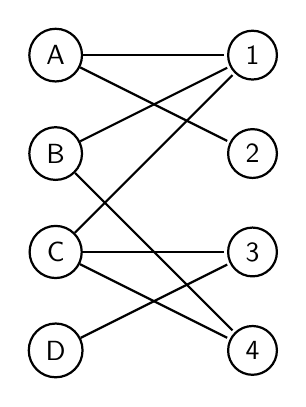
\begin{tikzpicture}[-,>=stealth,shorten >=1pt,auto,node distance=1.25cm,thick,main node/.style={scale=1,circle,draw,font=\sffamily\normalsize}]
            \node[main node] (A) []{A};
            \node[main node] (B) [below of = A]{B};
            \node[main node] (C) [below of = B]{C};
            \node[main node] (D) [below of = C]{D};

            \node[] (0) [right of = A]{};

            \node[main node] (1) [right of = 0]{1};
            \node[main node] (2) [below of = 1]{2};
            \node[main node] (3) [below of = 2]{3};
            \node[main node] (4) [below of = 3]{4};

            \path[every node/.style={font=\sffamily\small}]
                (A) edge (1)
                (B) edge (1)
                (C) edge (1)
                (A) edge (2)
                (C) edge (3)
                (D) edge (3)
                (B) edge (4)
                (C) edge (4)
                ;
        \end{tikzpicture}
    \end{center}
    
    Now, we add two nodes $S,T$ which we will refer to as the \textit{super-source} and the \textit{super-sink}. The super-source will be connected to each employee and the super-sink will be connected to each task. Additionally, we set the capacity of each edge to 1, ensuring that the matching between employees and the tasks is a bijection.

    \begin{center}
        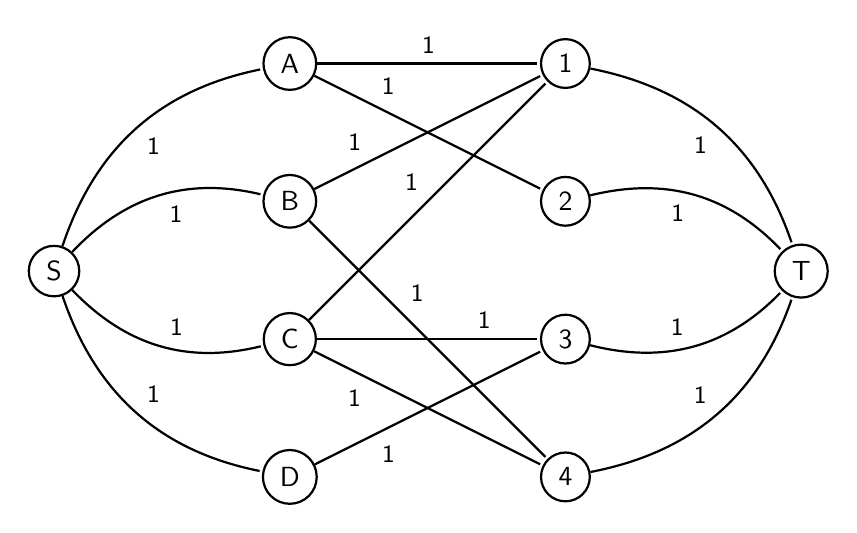
\begin{tikzpicture}[-,>=stealth,shorten >=1pt,auto,node distance=1.75cm,thick,main node/.style={scale=1,circle,draw,font=\sffamily\normalsize}]
            \node[main node] (A) []{A};
            \node[main node] (B) [below of = A]{B};
            \node[main node] (C) [below of = B]{C};
            \node[main node] (D) [below of = C]{D};

            \node[] (0) [right of = A]{};

            \node[main node] (1) [right of = 0]{1};
            \node[main node] (2) [below of = 1]{2};
            \node[main node] (3) [below of = 2]{3};
            \node[main node] (4) [below of = 3]{4};

            \node[main node] (S) [below left of = B, yshift=10, xshift=-50]{S};
            \node[main node] (T) [below right of = 2, yshift=10, xshift=50]{T};

            \path[every node/.style={font=\sffamily\small}]
                (S) edge[bend left, swap] node{1} (A)
                (S) edge[bend left, swap] node{1} (B)
                (S) edge[bend right] node{1} (C)
                (S) edge[bend right] node{1} (D)
                (A) edge node{1} (1)
                (B) edge[near start] node{1} (1)
                (C) edge node{1} (1)
                (A) edge[near start] node{1} (2)
                (C) edge[near end] node{1} (3)
                (D) edge[near start, swap] node{1} (3)
                (B) edge node[xshift=-10, yshift=10]{1} (4)
                (C) edge[near start, swap] node{1} (4)
                (1) edge[bend left,swap] node{1} (T)
                (2) edge[bend left,swap] node{1} (T)
                (3) edge[bend right] node{1} (T)
                (4) edge[bend right] node{1} (T)
                ;
        \end{tikzpicture}
    \end{center}

    Once the problem has been modeled as a network, it can easily be solved simply by applying the Edmonds-Karp algorithm: after finding the max flow, if the flow of the edge $(x,y)$ where $x \in \{A,B,C,D\}$ and $y \in \{1,2,3,4\}$ is set to 1 then the task $y$ gets assigned to the employee $x$.
    
    In some cases, not all tasks can be assigned. For example, if we add a fifth task then obviously one of the task will be unassigned since we have only 4 employees. Thus, the solution won't be a \textit{perfect matching}, but only a \textbf{maximal matching}, meaning that the found assignment maximizes the number of task that are assigned.

    Once we understood how to model the problem, we can also \textbf{vary its constraints}. For example, if we want to allow an employee to be able to work on more tasks at the same time, we can simply change the capacities outgoing from the super-source. Likewise, if we want to force that a task is executed by more than one employee, it's sufficient to change the ingoing super-sink capacities (of course, in this case we have to check that the super-sink edges are effectively filled).

    \begin{center}
        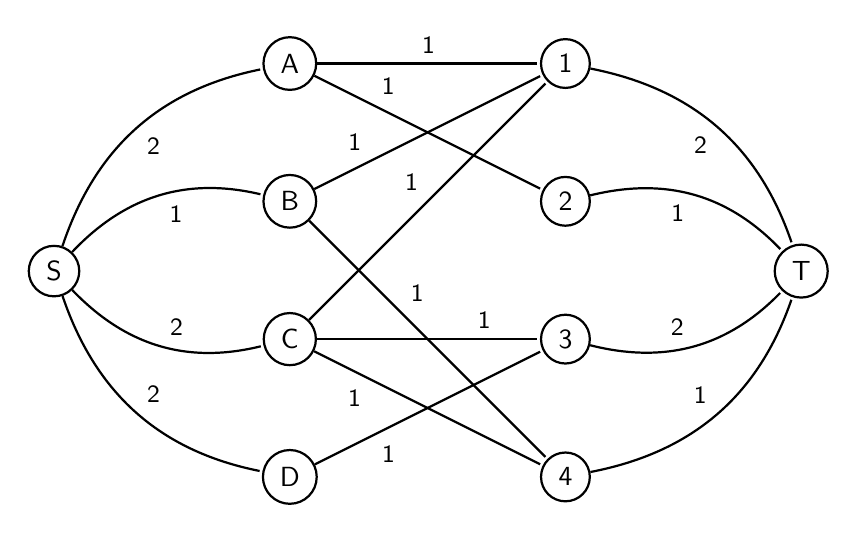
\begin{tikzpicture}[-,>=stealth,shorten >=1pt,auto,node distance=1.75cm,thick,main node/.style={scale=1,circle,draw,font=\sffamily\normalsize}]
            \node[main node] (A) []{A};
            \node[main node] (B) [below of = A]{B};
            \node[main node] (C) [below of = B]{C};
            \node[main node] (D) [below of = C]{D};

            \node[] (0) [right of = A]{};

            \node[main node] (1) [right of = 0]{1};
            \node[main node] (2) [below of = 1]{2};
            \node[main node] (3) [below of = 2]{3};
            \node[main node] (4) [below of = 3]{4};

            \node[main node] (S) [below left of = B, yshift=10, xshift=-50]{S};
            \node[main node] (T) [below right of = 2, yshift=10, xshift=50]{T};

            \path[every node/.style={font=\sffamily\small}]
                (S) edge[bend left, swap] node{2} (A)
                (S) edge[bend left, swap] node{1} (B)
                (S) edge[bend right] node{2} (C)
                (S) edge[bend right] node{2} (D)
                (A) edge node{1} (1)
                (B) edge[near start] node{1} (1)
                (C) edge node{1} (1)
                (A) edge[near start] node{1} (2)
                (C) edge[near end] node{1} (3)
                (D) edge[near start, swap] node{1} (3)
                (B) edge node[xshift=-10, yshift=10]{1} (4)
                (C) edge[near start, swap] node{1} (4)
                (1) edge[bend left,swap] node{2} (T)
                (2) edge[bend left,swap] node{1} (T)
                (3) edge[bend right] node{2} (T)
                (4) edge[bend right] node{1} (T)
                ;
        \end{tikzpicture}
        
    \end{center}

    \section{Solved exercises}

    \begin{framedprob}{}
        Suppose there are $n$ mice out on the field and there's a hungry owl about to make a move as soon as the owl can reach every single one of these mice. Scattered across the ground there are $k$ hole, each able to contain a certain number of mice. Every mouse is capable of running a maximum distance in any direction before being caught by the owl.
        
        Each mouse is identified by a triple $(x_i, y_i, d_i)$ describing its position and the maximum distance it can run, while hole is identified by a triple $(x_j, y_j, c_j)$ describing its position and its capacity, 
        
        Describe a way to find the maximum number of mice that can hide safely before being caught. 
    \end{framedprob}

    \textit{Solution:}

    First, we model the problem as a graph: for each mouse $m_i$ and each hole $h_j$ we add an edge $(m_i,h_j)$ if the mouse can reach the hole, i.e. if the maximum distance it can travel is less than the distance between it and the hole. Then, we proceed by adding a super-source node $s$, connected to each mouse, and a super-sink node $t$, connected to each hole.
    
    We set to 1 the capacity of each edge between $s$ and a mouse and each edge between a mouse and a hole. Similarly, we set the capacity of each edge between a hole and $t$ equal to the capacity of the hole itself. Finally, we apply the Edmonds-Karp algorithm on the described graph: the solution is given by the sum of the ingoing flows of the node $t$.

    \chapter{Linear programming}

    \section{Introduction and interpretation}

    \textbf{Linear programming}, also called \textit{linear optimization}, is a method to achieve the \textbf{optimal outcome} (such as maximum profit or lowest cost) in a mathematical model whose requirements and objective are represented by \textbf{linear inequalities}. In particular, the objective to be optimized is defined by an \textbf{objective function} on variables $x_1, \ldots, x_n$ that must be \textit{maximized} (or \textit{minimized}).

    For example, given two variables $x_1, x_2 \in \R$, we want to maximize the sum $x_1 + x_2$ while also respecting the following linear constraints:
    \[\begin{split}
        x_1 + 6x_2 & \leq 15 \\
        4x_1 - x_2 & \leq 10 \\
        x_2 - x_1 & \leq 1 \\
        x_1 & \geq 0 \\ 
        x_2 & \geq 0 \\
    \end{split}\]

    Since we have only two variables, these constraints can be interpreted as lines in a cartesian plane defined by $x_1$ and $x_2$: given a constraint $\alpha x_1 + \beta y_1 \leq \gamma$ (or $\alpha x_1 + \beta y_1 \geq \gamma$), the plane gets partitioned by the line $\alpha x_1 + \beta y_1 = \gamma$ and we can consider only the part that \textbf{respects the constraint}.

    By applying this process for each constraint, only one part of the graph will respect all the constraints. Any point in this area is a \textbf{feasible solution} to the problem. Furthermore, the area that contains the feasible solutions is called the \textbf{feasible region}.

    In particular, we want to find a feasible solution that maximizes (or minimizes) the objective function. These solutions are called \textbf{optimal solutions}. We notice now that the objective function $x_1 + 2x_2$ can also be rewritten as a scalar product:
    \[x_1 + x_2 = \smat{1 & 1} \cdot
    \smat{x_1 \\ x_2}\]

    \begin{figure}[H]
        \centering
        \includegraphics[scale=0.75]{images/lin_prog_1.png}
        \caption{The grey area is the feasible region defined by the constraints. The vector $\smat{1 & 1}$ shows the direction of the objective function to be maximized}
    \end{figure}

    Considering the line described by the vector $\smat{1 & 1}$, it's easy to see the optimal solution to the problem is given by the point \textbf{furthest from the origin}: the line \textit{perpendicular} to the vector $\smat{1 & 1}$ that passes through such point is the optimal solution.

    \begin{figure}[H]
        \centering
        \includegraphics[scale=0.75]{images/lin_prog_2.png}
        \caption{The optimal solution is given by the line $x_1+x_2 = 5$, meaning that $5$ is the optimal solution}
    \end{figure}

    \newpage

    In this problem, there is \textbf{only one optimal solution}, which is the vector $\smat{3 & 2}$. However, if vector that defines the direction of the objective function is \textit{perpendicular} to a constraint, we get \textbf{infinite optimal solutions} (because in $\R$ a segment has infinite points). 
    
    \begin{figure}[H]
        \centering
        \includegraphics[scale=0.75]{images/lin_prog_3.png}
        \caption{If the objective function is $\frac{1}{6}x_1 + x_2$, we get an infinite set of optimal solutions}
    \end{figure}


    Instead, if we reverse the directions of the inequalities of some of the constraints, we get that there is no feasible solution. Such programs are called \textbf{infeasible}.

    \begin{figure}[H]
        \centering
        \includegraphics[scale=0.75]{images/lin_prog_4.png}
    \end{figure}

    Finally, in some situations there may be a feasible solution but no optimal solution. These cases arise when the direction of the objective function is unbounded, meaning that we can always find a solution with a higher (or lower) value. Such programs are called \textbf{feasible unbounded}.

    \begin{figure}[H]
        \centering
        \includegraphics[scale=0.75]{images/lin_prog_5.png}
        \caption{If we remove some constraints, the program becomes feasible unbounded}
    \end{figure}

    \begin{framedprop}{Possibilities in a linear program}
        For each linear program, only one of the following cases holds:
        \begin{enumerate}
            \item The program is \textbf{infeasible}, meaning that there is no feasible solution
            \item The program is \textbf{feasible unbounded}, meaning that are infinite feasible solutions but no optimal solution
            \item The program is \textbf{uniquely optimal}, meaning that there are infinite feasible solutions and only one optimal solution
            \item The program is \textbf{infinitely optimal}, meaning that there are infinite optimal solutions
        \end{enumerate}
    \end{framedprop}

    Throughout the following sections and chapters, we will give proper justifications to formalize this result. Optimization problems are hidden in everyday life. For example, we can resolve the following two problems with linear programming:
    \begin{itemize}
        \item \textbf{Diet optimization}:
        
        Given $n$ types of food, for each $i$ such that $1 \leq n$ we define $x_i$ and $c_i$ respectively as the quantity and the cost of each food type $i$. Considering a set of nutritional constraints, such as minimum and maximum macro-nutrient intakes, we can define the following optimization problem in order to find the best combination of foods for our diet:
        \[\begin{array}{c}
            \min c_1 x_1 + \ldots + c_n x_n\\
            \\
            a_{1,1}x_1 + \ldots + a_{1,n}x_n \leq b_1 \\
            \vdots\\
            a_{m,1}x_1 + \ldots + a_{m,n}x_n \leq b_m \\
        \end{array}\]

        \item \textbf{Network flow}:
        
        Given a network $N = (G, s,t,c)$ and a flow $f$ on $N$, we can define a variable $x_{u,v}$ for all $(u,v) \in E(G)$ in order to formulate the max flow value problem as an optimization problem and find the optimal flow by setting $f(u,v) = x_{u,v}$. Trivially, each constraint of the network becomes a constraint of the problem.
    \end{itemize} 
    
    \quad

    \section{Linear programs and Standard form}

    In this section we give a proper formal definition of the concepts previously shown. Hence, it is assumed that each interpretation is already well-known.

    \begin{frameddefn}{Linear function}
        Let $\func{f}{\R^n}{\R}$. We say that $f$ is a \textbf{linear function} if
        \[\forall x,y \in \R^n, \forall \alpha, \beta \in \R \;\; f(\alpha x + \beta y) = \alpha f(x) + \beta f(y)\]
    \end{frameddefn}

    \begin{frameddefn}{Linear program}
        A \textbf{linear program}, or \textit{linear optimization problem}, is an optimization problem defined on an linear function $\func{f}{\R^n}{\R}$ to be maximized, called \textbf{objective function}, and constraints on the input vector $x$:
        \[\begin{array}{c}
            \max f(x) = c_1 x_1 + \ldots c_n x_n \\
            \\
            a_{1,1}x_1 + \ldots + a_{1,n}x_n \leq b_1 \\
            \vdots \\
            a_{m,1}x_1 + \ldots + a_{m,n}x_n \leq b_m \\
        \end{array}\]

        Each vector $x$ that respects the constraints is called a \textbf{feasible solution} and the set of feasible solutions is called \textbf{feasible region}. Each feasible solution that maximizes the objective function is called \textbf{optimal solution}.
    \end{frameddefn}

    In the previous section, we noticed how the objective function can also be rewritten as a scalar product:
    \[f(x) = c_1 x_1 + \ldots + c_n x_n = \smat{c_1 & \ldots & c_n}\smat{x_1 \\ \vdots \\ x_n}\]

    Thus, we can say that $f(x) = c^Tx$, where $c^T = \smat{c_1 & \ldots & c_n}$ is the transpose of the \textbf{coefficient vector of $f$}. Likewise, we notice that each constraint of the problem corresponds to a row of the linear system $Ax \leq b$. Thus, we can define the following \textbf{general formulation of linear programs}:

    \begin{framedprop}[label=conv_lin_prog]{Conversion of linear programs}
        Every linear program can be written as a maximization problem in the following general form:
        \[\begin{array}{c}
            \max \; c^Tx\\
            Ax \leq b\\
            x \geq 0
        \end{array}\]

        Through the following steps:
        \begin{enumerate}
            \item The optimal solution that minimizes $c^Tx$ also maximizes $-c^Tx$, so we can substitute $\min \; c^Tx$ with $\max \; -c^Tx$. \textbf{Warning}: even thought the solution is the same, the optimal value will have negated sign. This can be fixed by just inverting the negating optimal value.
            \item Any constraint of the form $a_1 x_1 + \ldots + a_n x_n \geq b$ is equivalent to the constraint $-a_1 x_1 - \ldots - a_n x_n \leq -b$, so we can substitute the first with the latter
            \item Any component variable $x_i$ such that $x < 0$ can be substituted with two non-negative variables $z_i, z_i' \geq 0$ such that $x_i = z_i- z_i'$
        \end{enumerate}
    \end{framedprop}

    Now, we would like to find a way to define the linear program in an \textbf{equational form}. In particular, consider the following linear program:
    \[\begin{array}{c}
        \max c_1x_1 + \ldots + c_nx_n\\
        \\
        a_{1,1}x_1 + \ldots + a_{1,n}x_n \leq b_1 \\
        \vdots \\
        a_{m,1}x_1 + \ldots + a_{m,n}x_n \leq b_m \\
    \end{array}\]
    where $A$ is the matrix formed by the constraints.

    We define $m$ variables $s_1, \ldots, s_m$, called \textbf{slack variables}, such that for each index $i = 1, \ldots, m$, we define $s_i := b_i - a_{1,1}x_1 + \ldots + a_{1,n}x_n$. By adding the slack variable $s_i$ to the left side of the $i$-th inequality, each inequality becomes an equality.

    Thus, \underline{at the cost of adding $m$ variables} to the problem, we can reformulate the problem as:
    \[\begin{array}{c}
        \max \; c_1x_1 + \ldots + c_nx_n + 0 \cdot s_1 + \ldots + 0 \cdot s_m\\
        \\
        a_{1,1}x_1 + \ldots + a_{1,n}x_n + s_1 = b_1 \\
        \vdots \\
        a_{m,1}x_1 + \ldots + a_{m,n}x_n + s_m = b_m \\
    \end{array}\]

    Given the $m \times m$ identity matrix $I_m$, we get that:
    \[\smat{A \mid I_m} \smat{x_1 \\ \vdots \\ x_n \\ s_1 \\ \vdots \\ s_m} = \smat{b_1 \\ \vdots \\ b_m }\]

    Then, by setting $A' := [A \mid I_m]$ and $c' := \smat{c_1 & \ldots & c_n & 0 & \ldots & 0}$ we get the following linear program in equational form:
    \[\begin{array}{c}
        \max \; c'^Tx\\
        A'x = b\\
        x \geq 0
    \end{array}\]

    \begin{frameddefn}{Standard form}
        A linear program is said to be in \textbf{standard form} (or \textit{equational form}) if it is formulated as:
        \[\begin{array}{c}
            \max \; c^Tx\\
            Ax = b\\
            x \geq 0
        \end{array}\]
        where $c,x \in \R^n$, $A \in \matspace{m}{n}{\R}$ and $b \in \R^m$.
    \end{frameddefn}
    
    Through \textit{linear algebra}, we can find numerous results involving linear programs in standard form. In particular, a fundamental result is that the system $Ax = b$ is \textbf{invariant under Gaussian row operations}. Thus, we can reduce the number of rows of $A$ through row elimination in order to obtain the \textbf{minimal amount of constraints} that define the problem. For these reasons, we are going to assume that each removable row has already been removed, meaning that the \textbf{rows} (but always not the columns) of $A$ are assumed to be \textbf{linearly independent}. Moreover, since we generally obtain a standard form linear program from a non-standard one and the transformation adds $m$ variables to the problem, we're going to always assume that $m \leq n$.

    \begin{framedobs}{Assumptions on standard form LPs}
        Given a linear program in standard form $Ax=b$ with $x \geq 0$, we assume that:
        \begin{itemize}
            \item $A \in \matspace{m}{n}{\R}$ and $m \leq n$
            \item The rows of the matrix $A$ are always linearly independent
            \item The rank of $A$ is $\mathrm{rank}(A) = \mathrm{colrank}(A) = \mathrm{rowrank}(A)  = m$
        \end{itemize}
    \end{framedobs}

    \newpage

    \section{Basic feasible solutions}

    Among all the feasible solutions of a linear program, a privileged status is granted to so-called \textbf{basic feasible solutions}. First, we'll give a geometric intuition of these types of feasible solutions: a basic feasible solution is a \textit{vertex} (or corner, spike) of the set of feasible solutions.

    \begin{figure}[H]
        \centering
        \includegraphics[scale=0.85]{images/bfs.png}
        \caption{A set of feasible solutions}
        \label{bfs}
    \end{figure}

    For example, in the set of feasible solutions shown above in grey, among $p$, $q$ and $r$ only the latter is basic. In particular, we notice that the solution $r$ is set to zero on both the $x_2$ and $x_3$ axes. In fact, very roughly speaking, a basic feasible solution is a feasible solution with sufficiently many variables set to zero. This intuition will be justified later both informally and formally.

    First of all, we will introduce some new notation: consider a linear program in standard form:
    \[\begin{array}{c}
        \max \;\, c^Tx\\
        Ax = b\\
        x \geq 0
    \end{array}\]
    where $A \in \mathrm{Mat}_{m \times n}$ and we denote with $A = (A^1, \ldots, A^n)$ the column decomposition of $A$. Given a subset of indices $\B \subseteq \{1, \ldots, n\}$ called \textbf{basis}, we define the matrix $A_\B$ as the \textbf{matrix formed by the columns of $A$} whose index is inside $\B$, meaning that $A_\B = (A^{i_1}, \ldots, A^{i_k})$ where $i_1, \ldots, i_k \in \B$.

    \textbf{Example:}

    \begin{itemize}
        \item Suppose that:
        \[A = \smat{
            1 & 6 & 3 & -3 & 4 \\
            0 & 1 & 3 & 2 & 4
        }\]

        If $\B = \{2,4\}$, the matrix $A_\B$ is equal to:
        \[A_\B = \smat{
            6 & -3 \\
            1 & 2
        }\]
    \end{itemize}

    \newpage

    \begin{framedprop}{}
        Given the matrix equation $Ax = b$ and a subset of indices $\B \subseteq \{1, \ldots, n\}$, if $\abs{\B} = m$ and $A_\B$ is \textit{non-singular}, meaning that $\det(A_\B) \neq 0$, then there exists a solution $\overline{x} := (x_1, \ldots, x_n) \in \R^n$ such that $A \overline{x} = b$  and $\forall i \notin \B \;\, x_i = 0$.
    \end{framedprop}

    \proofenv{

        If $\abs{B} = m$ and $\det(A_\B) \neq 0$ then $A_\B$ is a non-singular $m \times m$ matrix with rank $m$. Thus, through the \textit{Rouché-Capelli theorem}, since $A_\B$ is also a minor of both $A$ and $(A \mid b)$, we get that $\mathrm{rank}(A) = \mathrm{rank}(A \mid b) = m$, implying that subspace of solutions of $Ax = b$ has rank $n-m$. Moreover, since the columns whose index isn't in $\B$ are linearly dependent by the other columns, this subspace will always contain a solution such that $\forall i \notin \B \;\, x_i = 0$.

    }

    \begin{frameddefn}{Basic feasible solution}
        Given the equation $Ax = b$ of a standard form linear program, we say that $\overline{x} \in \R^n$ is a \textbf{basic feasible solution (BFS)} if $\overline{x}$ is a feasible solution for which there exists an index set $\B \subseteq \{1, \ldots, n\}$ such that:
        \begin{itemize}
            \item $A_\B$ is an $m \times m$ non-singular matrix
            \item $\forall i \notin \B \;\; \overline{x_i} = 0$
        \end{itemize}

        Moreover, we say that $\B$ \textbf{certifies} $\overline{x}$ and call \textbf{basic variable} each variable $x_i$ such that $i \in \B$, while the other variables are called \textbf{non-basic variable}.
    \end{frameddefn}

    \textbf{Example:}
    \begin{itemize}
        \item Suppose that a standard form linear program is defined by:
        \[A = \smat{
            1 & 6 & 3 & -3 & 4 \\
            0 & 1 & 3 & 2 & 4
        } \qquad\qquad b = \smat{6 \\ 6}\]

        If $\B = \{2,4\}$, the matrix $A_\B$ is equal to:
        \[A_\B = \smat{
            6 & -3 \\
            1 & 2
        }\]
        
        Furthermore, since $\det(A_\B) = 15 \neq 0$ and $\abs{\B} = 2$, we know that there exists a vector $\overline{x}^T = \smat{x_1 & x_2 & x_3 & x_4 & x_5}$ such that $A\overline{x} = b$. By solving the following equation
        \[\smat{
            6 & -3 \\
            1 & 2
        } \smat{x_2 \\ x_4} = \smat{6 \\ 6}\]
        
        we get that $x_2 = 2$ and $x_4 = 2$. Finally, by setting all the other variables to 0, we get that the vector $\overline{x}^T = \smat{0 & 2 & 0 & 2 & 0}$ implies that $\overline{x}$ is a BFS.

        An important thing to notice is that $\overline{x}$ is a BFS because it also respects the constraint of non-negative solutions since $\overline{x} \geq 0$, meaning that it is indeed a feasible solution. The method that was just shown doesn't always guarantee that the solution to the "reduced equation" is also a feasible solution.

        For example, if we consider $\B' = \{1,2\}$, we get that $\det(A_{\B'}) = -5 \neq 0$ and $\abs{\B'} = 2$, so we know that there exists a vector $\overline{y}^T = \smat{y_1 & y_2 & y_3 & y_4 & y_5}$ such that $A\overline{y} = b$. However, by solving the following equation
        \[\smat{
            1 & 6 \\
            0 & 1
        } \smat{y_1 \\ y_3} = \smat{6 \\ 6}\]
        we get that $y_1 = -30$ and $y_2 = 6$, the vector $\overline{y}^T = \smat{-30 & 6 & 0 & 0 & 0}$ doesn't respect the constraint $\overline{y} \geq 0$, meaning that it isn't a feasible solution and by consequence that it isn't a BFS.

    \end{itemize}
    
    \begin{framedthm}[label=bfs_if_AK_lin_ind]{}
        Given a feasible solution $\overline{x} = \smat{x_1 & \ldots & x_n}$ to a linear program, let $K = \{i \in \{1, \ldots, n\} : x_i > 0\}$. It holds that:
        \[\overline{x} \text{ is a BFS} \iff \text{Columns of $A_K$ are lin. ind.}\]
    \end{framedthm}

    \proofiff{
        Suppose that $\overline{x}$ is a BFS and let $\B$ be the basis through which we obtain $\overline{x}$. Every non-basic variable of $\overline{x}$ is set to $0$, meaning that $\forall i \notin \B$ we have that $x_i = 0$. However, since for all the other basic variables $x_j$ it holds that $x_j \geq 0$, these variables could also be set to 0.
            
        Thus, generally we have that $K \subseteq \B$. Since $A_\B$ is non-singular, the columns of $A_\B$ are linearly independent. Then, since $i \in K \subseteq \B$, each column of the matrix $A_K$ is also linearly independent.
    }{
        Suppose that the columns of $A_K$ are linearly independent, implying that $\det(A_K) \neq 0$. If $\abs{K} = m$ then $K$ certifies that $\overline{x}$ is a BFS.
        If $\abs{K} < m$, instead, we pick $\B \subseteq \{1, \ldots, n\}$ such that:
        \begin{itemize}
            \item $K \subseteq \B$
            \item $A_\B$ has linearly independent columns
            \item $\B$ is as big as possible
        \end{itemize}

        Such set $\B$ always exists since, eventually, $K = \B$ is allowed by definition.

        Since the columns of $A_\B$ are also columns of $A$, since $\B$ is as big as possible and since $A_\B$ is has linearly independent columns, it holds that $\mathrm{rank}(A_\B) = \mathrm{rank}(A) = m$, implying that $\abs{\B} = m$ and thus that $\B$ certifies that $\overline{x}$ is a BFS.
    }

    \begin{framedobs}{}
        A BFS can be certified by \underline{more than one basis}
    \end{framedobs}

    \textbf{Example:}
    \begin{itemize}
        \item Suppose that a standard form linear program is defined by:
        \[A = \smat{
            1 & 6 & 3 & -3 & 4 \\
            0 & 1 & 3 & 2 & 4
        } \qquad\qquad b = \smat{6 \\ 6}\]

        By the previous theorem, the vector $\overline{x}^T = \smat{0 & 0 & 2 & 0 & 0}$ gives a BFS due to the fact that $K = \{3\}$ and the columns of $A_K$ are clearly linearly independent since it is made of only one column. Moreover, we notice that we can expand the set $K$ to two different basis $\B = \{1,3\}$ and $\B' = \{2,3\}$
    \end{itemize}

    \begin{frameddefn}{Feasible basis}
        Given a basis $\B$ of a linear program, we say that $\B$ is \textbf{feasible} if it certifies a BFS
    \end{frameddefn}

    \begin{framedobs}[label=unique_bfs]{}
        Given a feasible basis $\B$, there exists \underline{only one} BFS $\overline{x}$ certified by $\B$
    \end{framedobs}

    \proofenv{

        Let $\B = \{i_1, \ldots, i_k\}$. Since $\B$ is a feasible basis, the matrix $A_\B$ is made of linearly independent columns, implying that there must be only one solution to the equation
        \[A_\B \cdot \smat{x_{i_1} \\ \vdots \\ x_{i_k}} = b\]
    }

    \begin{framedprop}{}
        A linear program in standard form has at most $\binom{n}{m}$ BFS
    \end{framedprop}

    \proofenv{

        Since each basis must have cardinality $m$ and since $A$ has $n$ columns, the number of possible choises for a basis is $\binom{n}{m}$. Then, even if all the possible basis are feasible basis each one of them corresponds to only one BFS which could also be shared with another basis. Thus, even if no BFS is shared among more than one basis, there can be at most $\binom{n}{m}$ BFSs.

    }

    \newpage

    \subsection{Above bounded linear programs and BFS}

    \begin{frameddefn}{Above bounded linear program}
        Given a linear program in standard form, we say that it's objective function is \textbf{bounded above} if $\exists N \in \R$ such that for all feasible solutions $y$ it holds that $c^Ty \leq N$.
    \end{frameddefn}

    \begin{framedthm}{}
        Given a linear program in standard form, if the objective function has an upper bound then for each feasible solution $y$ there exists a BFS $z$ such that $c^Tz \geq c^Ty$.
    \end{framedthm}

    \proofenv{

        Let $y$ be a feasible solution and let $z$ be a feasible solution with the maximum amount of zero variables and such that $c^Tz \geq c^Ty$. Such a feasible solution $z$ always exists since, eventually, $y = z$ is allowed by definition.

        By way of contradtiction, suppose that $z$ isn't a BFS and let $K = \{i \in \{1, \ldots, n\} \mid z_i > 0\}$. It's easy to see that the columns of $A_K$ must be linearly dependent: if they weren't, by theorem \cref{bfs_if_AK_lin_ind} we would get that $z$ is a BFS, which is impossible.
        
        Since they are linearly dependent, we know that $\exists \alpha_{i_1}, \ldots, \alpha_{i_k} \neq 0$, where $K = \{i_1, \ldots, i_k\}$, such that
        \[\alpha_{i_1}A^{i_1}_K + \ldots + \alpha_{i_k} A^{i_k}_K = 0 \iff A_K \cdot \smat{\alpha_{i_1} \\ \vdots \\ \alpha_{i_1}} = 0\]

        Since the columns of $A_K$ are also columns of $A$ and since the coefficients $\alpha_{i_1}, \ldots, \alpha_{i_k}$ nullify the linear combination of the columns in $A_K$, by setting to 0 the coefficient of every other column of $A$ we can nullify the linear combination of the columns of $A$. 

        Then, let $w$ such vector of coefficients, formally defined as:
        \[w_j = \soe{ll}{
            a_j &\text{if } j \in K \\
            0 & \text{otherwise}
        }\]

        As we just said, we know that $Aw = 0$.

        \textbf{Claim}: We can assume that the vector $w$ satisfies the following two conditions:
        \begin{enumerate}
            \item $c^Tw \geq 0$
            \item $\exists j \in K$ such that $w_j < 0$        
        \end{enumerate}
        
        \proofenv[Proof of the claim]{
                
            First, we notice that $Aw = 0$, for all $\beta \in \R$ it also holds that $A(\beta w) = 0$.
            
            If $c^Tw = 0$ then $c^Tw \geq 0$ trivially holds. Moreover, if the second condition doesn't hold for $w$, meaning that $\forall j \in K$ we have that $w_j \geq 0$, we can substitute $w$ with the vector $-w$, satisfying the second condition since $w \neq 0$. In particular, we notice that such substitution doesn't violate the first condition: if $c^Tw = 0$, by linearity of the objective function it holds that $c^T(-w) = -(c^T w) = 0$.

            If $c^Tw \neq 0$, by picking $w$ or $-w$ we can satisfy the first condition since $c^Tw > 0$ or $c^T(-w) > 0$ must hold. Without loss of generality, in the following statements we will assume that $w$ was chosen.
            
            By way of contradiction, suppose that the second condition doesn't hold, meaning that $\forall j \in K$ we have that $w_j \geq 0$.

            Given $t \in \R$ such that $t \geq 0$, let $z(t) := z + tw$. We notice that $z(0) = z$ and that
            \[A \cdot z(t) = A(z + tw) = Az + tAw\]
            
            Since $z$ is a feasible solution, meaning that $Az = b$, and since $Aw = 0$, we get that $A \cdot z(t) = b$. Furthermore, since $z$ is a feasible solution and since by assumption $\forall j \in K \;\; w_j \geq 0$, for each index $i$ we know that $z(t)_i = z_i + tw_i \geq 0$, concluding that $z(t) \geq 0$ and thus that it is indeed a feasible solution.

            By linearity of the objective function, we also know that:
            \[c^T \cdot z(t) = c^T(z+tw) = c^Tz + tc^Tw\]

            Since $t \geq 0$ and since $c^T > w$, we also get that $tc^Tw > 0$. However, this is valid $\forall t \in \R$, meaning that we can always choose a value $t'$ bigger than the previous for which $c^{t'}w > c^tw$, contradicting the fact that the objective function has an upper bound. Thus, it must be true that $\exists j \in K$ such that $w_j < 0$.
        }

        Once this assumption is made, given $t \in \R$ we define again the vector $z(t) := z + tw$.
        As before, we notice that $A \cdot z(t) = b$. However, it is no longer always true that $z(t) \geq 0$ since we proved that $\exists j \in K$ such that $w_j < 0$ (that result was given by assuming the contrary). In fact, if $t > \frac{z_i}{-w_i}$ we get that $z(t)_i < 0$.

        \textbf{Claim}: $\exists t' > 0$ such that $z(t')$ is a feasible solution with more zeros than $z$

        \proofenv[Proof of the claim]{
            Since $z$ is a feasible solution, we know that $z \geq 0$. Furthermore, we recall that $K$ is defined as $K = \{i \in \{1, \ldots, n\} : z_i > 0\}$, implying that for each $j \notin K$ it must be true that $z_j = 0$. 
            
            Thus, since for $j \notin K$ we also know that $w_j = 0$, we get that:
            \[z(t)_j = \soe{ll}{
                z_j + tw_j & \text{if } j \in K \\
                0 & \text{otherwise} \\
            }\] 
            
            Since $\exists h \in K$ such that $w_h < 0$, let $t' = \min\limits_{h \in K : w_h < 0}\rbk{\frac{z_j}{-w_j}}$. In particular, notice that by the way $t'$ is defined we get that:
            \begin{itemize}
                \item By choice of $h$, we know that $z_h > 0$ and $w_h < 0$, thus $t' > 0$
                \item If $z_i = 0$ then $i \notin K$, implying also that $z(t')_i = 0$. However, by choice of $h$, we know that $z_h > 0$
                \[z(t')_h = z_h + t'w_h = z_h + \frac{z_j}{-w_j} \cdot w_j = 0\]
                thus $z(t')$ always has at least one more zero variable than $z$

                \item Since $t' > 0$, for each $j \in K$ such that $w_j < 0$ it holds that:
                \[t' = \frac{z_h}{-w_h} \leq \frac{z_j}{-w_h} \implies t'w_j \geq z_j\]
            \end{itemize}

            Given an index $i$, if $i \notin K$ then we already know that $z(t')_i = 0$. If $i \in K$, instead, by definition of $K$ we get that $z_i > 0$. Thus, we get two additional subcases:
            \begin{itemize}
                \item If $w_i \geq 0$ then $z(t')_i = z_i + t'w_i \geq 0$
                \item If $w_i < 0$ then $t'w_i < 0$, but we also know that $t'w_i \geq z_i$, implying that $z(t')_i = z_i + t'w_i \geq 0$
            \end{itemize}

            Thus in all cases we get that $z(t') \geq 0$. Since it's also true that $A \cdot z(t') = b$, this concludes that $z(t')$ is a feasible solution with more zeros than $z$
        }
        
        Finally, by linearity of the objective function and since we showed that $c^Tw \geq 0$ and $t' > 0$, we get that
        \[c^T \cdot z(t') = c^T(z+t'w) = c^Tz + t'c^Tw \geq c^Tz \geq c^Ty\]
        
        Thus, we get that $z(t')$ is a feasible solution with more zeros than $z$ and such that $c^T \cdot z(t') \geq c^Ty$, contradicting our initial assumption for which $z$ was chosen with such characteristics. Thus, it must be impossible for $z$ to not be a BFS.
        
    }

    \begin{framedcor}{Feasible solution with maximum zeros}
        A BFS is a feasible solution with the \textbf{maximum amount of zero variables}. Thus, if there is at least one feasible solution, there also is at least one BFS.

        \textit{(follows from the way we proved the previous theorem)}
    \end{framedcor}

    This corollary only partially justifies the previously mentioned geometric intuitions. In fact, we now know that a BFS has a sufficient amount of zero components. However, this isn't enough to justify that it is a tip of the set of feasible solutions: if we consider the image shown in \cref{bfs}, a point on the segment between the origin and $r$ also has the components $x_2$ and $x_3$ set to zero. In the following sections, we will discuss how these points can't be a BFS due to not being a tip.

    \newpage

    \begin{framedthm}[label=opt_sol_bfs]{}
        Given a linear program in standard form, it holds that:
        \begin{enumerate}
            \item If there is at least one feasible solution and the objective function has an upper bound, there also is at least one \textbf{optimal solution}
            \item If there is an optimal solution, there also is a \textbf{BFS that is optimal}
        \end{enumerate}
    \end{framedthm}

    \proofenv{
        \begin{enumerate}
            \item Suppose that there is at least a feasible solution $y$ and that the objective function has an upper bound. Through the previous theorem, we know that there is a BFS $z$ such that $c^Tz \geq c^Ty$. Thus, there is at least one BFS.
            
            Since there are at most $\binom{n}{m}$ BFSs, let $\overline{x}$ be the BFS such that:
            \[c^T\overline{x} = \max_{z \text{ BFS}}(c^Tz)\]

            By way of contradiction, suppose that $\overline{x}$ isn't optimal, implying that there is at least another feasible solution $\overline{z}$ such that $c^T\overline{z} > c^T \overline{x}$.
            
            Again, through the previous theorem we know that there also exists a BFS $\overline{y}$ such that $c^T\overline{y} \geq c^T \overline{z}$. However, this would also imply that $c^T\overline{y} \geq c^T \overline{z} > c^T\overline{x}$, which contradicts the fact that $\overline{x}$ was chosen as the BFS with maximal objective function value. Thus, it must be true that $\overline{x}$ is optimal and thus that there is at least one optimal solution.

            \item Suppose that there is an optimal solution $\overline{x}$. Then, by the previous theorem, we know that there is a BFS $\overline{y}$ such that $c^T\overline{y} \geq c^T \overline{x}$.
            
            However, since $\overline{x}$ is optimal, it's also true that $c^T\overline{x} \geq c^T \overline{y}$. Thus, $c^T\overline{x} = c^T \overline{y}$, concluding that $\overline{x}$ must also be an optimal solution.
        \end{enumerate}
    }

    \newpage

    \section{Geometry behind linear programs}

    \subsection{Convexity}

    In this section we will formally define the geometric intuitions behind linear programs. These geometric concepts are fundamental to define methods and algorithms that can solve linear programs efficiently.

    \begin{frameddefn}{Convex set}
        Let $X \subseteq \R^n$. We say that $X$ is \textbf{convex} if $\forall x_1,x_2 \in X$ it holds that all the points in the line segment from $x_1$ to $x_2$ are also in $X$.

        Formally, this means that $\forall x_1, x_2 \in X$ and $\forall \alpha \in [0,1] \subset \R^n$ it holds that the linear combination $\alpha x_1 + (1-\alpha) x_2$ is also in $X$.
    \end{frameddefn}

    \begin{center}
        \begin{tabular}{ccc}
            \textbf{Convex} && \textbf{Non-Convex}\\
            \includegraphics[scale=0.6]{images/convex.png}
            &\qquad\qquad&
            \includegraphics[scale=0.6]{images/non-convex.png}
        \end{tabular}
    \end{center}

    \begin{framedprop}[label={fis_convex}]{}
        The \textbf{feasible region} of every linear program is a \textbf{convex set}. 
    \end{framedprop}

    \proofenv{

        Suppose that the following inequalities are the constraints of a linear program:
        \[\begin{array}{c}
            a_{1,1}x_1 + \ldots + a_{1,n}x_n \leq b_1 \\
            \vdots \\
            a_{m,1}x_1 + \ldots + a_{m,n}x_n \leq b_m \\
        \end{array}\]

        Let $X$ be the feasible region of the linear program. Let $\overline{x} := (\overline{x_1}, \ldots, \overline{x_1})$ and $\overline{y} := (\overline{y_1}, \ldots, \overline{y_1})$ be two feasible solutions, meaning that $\overline{x}, \overline{y} \in X$.

        Given $\gamma \in [0,1] \subset \R^n$, we notice that:
        \[\begin{array}{c}
            \gamma(a_{1,1}\overline{x_1} + \ldots + a_{1,n}\overline{x_n}) \leq \gamma b_1 \\
            \vdots \\
            \gamma(a_{m,1}\overline{x_1} + \ldots + a_{m,n}\overline{x_n}) \leq \gamma b_m \\
        \end{array} \implies 
        \begin{array}{c}
            a_{1,1}(\gamma \overline{x_1}) + \ldots + a_{1,n} (\gamma \overline{x_n}) \leq \gamma b_1 \\
            \vdots \\
            a_{m,1}(\gamma \overline{x_1}) + \ldots + a_{m,n} (\gamma \overline{x_n}) \leq \gamma b_m \\
        \end{array}\]

        Likewise, we can show that:
        \[\begin{array}{c}
            a_{1,1}((1-\gamma)\overline{y_1}) + \ldots + a_{1,n} ((1-\gamma)\overline{y_n}) \leq (1-\gamma) b_1 \\
            \vdots \\
            a_{m,1}((1-\gamma)\overline{y_1}) + \ldots + a_{m,n} ((1-\gamma)\overline{y_n}) \leq (1-\gamma) b_m \\
        \end{array}\]

        Thus, by summing the two systems of inequalities, we get that:
        \[\begin{array}{c}
            a_{1,1}(\gamma \overline{x_1} + (1-\gamma)\overline{y_1}) + \ldots + a_{1,n} (\gamma \overline{x_n} + (1-\gamma)\overline{y_n}) \leq b_1 \\
            \vdots \\
            a_{m,1}(\gamma \overline{x_1} + (1-\gamma)\overline{y_1}) + \ldots + a_{m,n} (\gamma \overline{x_n} + (1-\gamma)\overline{y_n}) \leq b_m \\
        \end{array}\]

        concluding that $\gamma \overline{x} + (1-\gamma) \overline{y}$ is also a feasible solution and thus that it's in $X$

    }

    \begin{framedobs}{Infinite optimal solutions}
        Given a linear program, if there are two distinct optimal solutions $\overline{x}, \overline{y}$ then there are infinite optimal solutions.
    \end{framedobs}

    \proofenv{
        
        Let $\beta$ be the maximum value of the objective function $f$ obtained with the optimal solutions $\overline{x}, \overline{y}$, meaning that $f(\overline{x}) = f(\overline{y}) = \beta$. For each $\alpha \in [0,1] \subset \R^n$, we know that $\alpha \overline{x} + (1-\alpha) \overline{y}$ is a feasible solution due to the feasible region being a convex set.

        Furthermore, by linearity of $f$, we notice that:
        \[f(\alpha \overline{x} + (1-\alpha) \overline{y}) = \alpha f(\overline{x}) + (1-\alpha) f(\overline{y}) = \alpha \beta + (1- \alpha) \beta = \beta\]
        concluding that $\forall \alpha \in [0,1] \subset \R^n$ we get that $\alpha \overline{x} + (1-\alpha) \overline{y}$ is also an optimal solution.

    }

    \begin{framedobs}{Intersection of convex sets}
        Given two convex sets $X, Y \subseteq \R^n$, the intersection $X \cap Y$ is also convex
    \end{framedobs}

    \proofenv{

        Given $u,v \in X \cap Y$, we know that each point in the segment between $u$ and $v$ is both in $X$ and $Y$ due to the convexity of $X$ and $Y$, implying that the segment is also in $X \cap Y$.

    }

    \newpage

    \begin{frameddefn}{Convex hull}
        Given $x_1, \ldots, x_n \in \R^n$, a \textbf{convex hull} of $x_1, \ldots, x_n$ is the intersection of all the convex sets $X_1, X_2, \ldots \subseteq \R^n$ that contain $x_1, \ldots, x_n$.
    \end{frameddefn}

    By the previous observation, its obvious that the convex hull is also convex. Moreover, intuitively by definition we get that the convex hull is the minimal convex set that contains $x_1, \ldots, x_n$.

    \begin{figure}[H]
        \centering
        \includegraphics[scale=0.75]{images/convex_hull.png}
        \caption{Example of convex hull}
    \end{figure}
    
    Even though this definition is intuitive enough, it isn't very constructive. In fact, we can also define the convex hull in terms of \textit{convex combinations}, a generalization of the formal definition of a segment between two points.
    
    \begin{frameddefn}{Convex combination}
        Given $x_1, \ldots, x_n \in \R^n$, a \textbf{convex combination} of $x_1, \ldots, x_n$ is a linear combination $z$ with non-negative coefficients such that the sum of the coefficients equals one.
        
        Formally, it corresponds to a vector $z$ such that:
        \begin{itemize}
            \item $z = \sum\limits_{i = 1}^n a_i x_i$
            \item $\sum\limits_{i = 1}^n a_i = 1$
            \item $a_1, \ldots, a_n \geq 0$
        \end{itemize}
    \end{frameddefn}

    \begin{figure}[H]
        \centering
        \includegraphics[scale=0.1]{images/convex_combination.png}
        \caption{The point $P$ is a convex combination of $x_1, x_2, x_3$, while $Q$ is not}
    \end{figure}

    \newpage

    \begin{framedprop}[label=convex_hull_combinations]{}
        Given $x_1, \ldots, x_n \in \R^n$, the convex hull of $x_1, \ldots, x_n$ is equal to the set of convex combinations of $x_1, \ldots, x_n$
    \end{framedprop}

    \proofenv{

        Let $C$ be the convex hull of $x_1, \ldots, x_n$ and let $\tilde{C}$ be the set of convex combinations, meaning that:
        \[\tilde{C} = \cbk{\sum\limits_{i = 1}^n a_i x_i \left | \sum\limits_{i = 1}^n a_i = 1 \;\text{ and }\; a_1, \ldots, a_n \geq 0 \right .}\]

        Given $u,v \in \tilde{C}$, we know that:
        \[u = \sum_{i = 1}^n a_i x_i \qquad \qquad v = \sum_{i = 0}^n b_i x_i\]
        where $\sum\limits_{i = 1}^n a_i = \sum\limits_{i = 1}^n b_i = 1$ and $a_1, \ldots, a_n, b_1, \ldots, b_n \geq 0$.

        Given $\gamma \in [0,1] \subseteq \R^n$, let $z := \gamma u + (1- \gamma) v$. We notice that:
        \[\begin{split}
            z &= \gamma u + (1-\gamma) v \\
             &= \gamma \sum_{i = 1}^n a_i x_i + (1-\gamma) \sum_{i = 1}^n b_i x_i \\
             &= \sum_{i = 1}^n (\gamma a_i + (1-\gamma) b_i) x_i \\
             &= \sum_{i = 1}^n c_i x_i
        \end{split}\]

        where $c_i := \gamma a_i + (1-\gamma) b_i$. Since for each index $i$ we have that $\gamma, (1-\gamma), a_i, b_i \geq 0$, it's also true that $c_i \geq 0$. Finally, we notice that:
        \[\begin{split}
            \sum_{i = 1}^n c_i &= \sum_{i = 1}^n (\gamma a_i + (1-\gamma) b_i) \\
            &= \gamma \sum_{i = 1}^n a_i + (1-\gamma) \sum_{i = 1}^n b_i \\
            &= \gamma \cdot 1 + (1-\gamma) \cdot 1 \\
            &= 1
        \end{split}\]

        Thus, we conclude that $\tilde{C}$ is convex. In particular, we notice that for each index $i$ it holds that:
        \[x_i = 0 \cdot x_1 + \ldots 0 \cdot x_{i-1} + 1 \cdot x_i + 0 \cdot x_{i+1} + \ldots 0 \cdot x_n\]
        implying that $x_1, \ldots, x_n \in \tilde{C}$, meaning that $\tilde{C}$ is a convex that contains $x_1, \ldots, x_n$. Then, by definition of convex hull, it must hold that $C \subseteq \tilde{C}$.
        
        Vice versa, we know show that $\tilde{C} \subseteq C$. Given $z \in \tilde{C}$, we know that $z = \sum\limits_{i = 1}^n d_i x_i$ where $\sum\limits_{i = 1}^n d_i = 1$ and $d_1, \ldots, d_n \geq 0$. By induction, we show that for each $m \in \N$ such that $1 \leq m \leq n$, if the number of coefficients greater than 0 that compose $z$ equals $m$ then it holds that $z \in C$.
        
        For the base case, it's easy to see that if $m = 1$ then there is only one index $i$ such that $d_i > 0$, while for every other index $j \neq i$ it holds that $d_j = 0$. Then, since the sum of all the coefficients must be equal to one, this can hold only if $d_i = 1$, meaning that $z = x_i$ and thus that $z \in C$ by definition of convex hull.

        Assuming that the statement holds for each point in $\tilde{C}$ with $m-1$ coefficients greater than zero, suppose that $z$ has $m$ coefficients $i_1, \ldots, i_m$ such that $d_{i_1}, \ldots, d_{i_m} > 0$. Given $j \in \{i_1, \ldots, i_m\}$, we notice that:
        \[\sum_{i = 1}^n d_i = 1 \implies \sum_{\substack{i = 1,\\ i \neq j}}^n d_i = 1-d_j \implies \sum_{\substack{i = 1,\\ i \neq j}}^n \frac{d_i}{1-d_j} = 1 \] 
        
        For each index $i$, we define $k_i$ as:
        \[k_i = \soe{ll}{
            \frac{d_i}{1-d_j} & \text{if } i \neq j \\
            0 & \text{otherwise}
        }\] 
        
        Let $w = \sum\limits_{i = 0}^n k_i x_i$. We notice that, by definition of each $k_i$, it holds that
        \[\sum\limits_{i = 0}^n k_i = k_j + \sum_{\substack{i = 1,\\ i \neq j}}^n \frac{d_i}{1-d_j} = 1\]

        Moreover, since $d_{i_1}, \ldots, d_{i_m} > 0$, by definition of each $k_i$ we know that $k_{i_1}, \ldots, k_{j-1}, k_{j+1}, \\\ldots, k_{i_m} > 0$, meaning that $w$ has $m-1$ coefficients greater than zero. Thus, by inductive hypothesis we know that $w \in C$.

        Finally, we notice that:
        \[z = \sum_{i = 1}^n d_i x_i = d_j x_j + \sum_{\substack{i = 1,\\ i \neq j}}^n d_i x_i = d_j x_j + (1-d_j) w\]
        meaning that $z$ is part of the segment between $x_j$ and $w$. Thus, since $C$ is convex and since $x_j, w \in C$, it must also be true that $z \in C$. Then, since we showed that this holds for each vector with any possible amount of coefficients with value greater than zero, this holds for all points in $\tilde{C}$, concluding that $\tilde{C} \subseteq C$.

    }

    \newpage

    After giving a proper definition of convex hull, we can give a clearer picture of what's going on: given $x_1, \ldots, x_n \in \R^n$, assuming that the vectors are \textit{linearly independent}, we get that:
    \begin{itemize}
        \item If $n = 2$ then the set of convex combinations corresponds to a segment between $x_1$ and $x_2$
        \item If $n = 3$ then the set of convex combinations corresponds to a convex bounded polygon with vertices $x_1, x_2$ and $x_3$
        \item If $n = 4$ then the set of convex combinations corresponds to a convex  bounded polyhedron with vertices $x_1, x_2, x_3$ and $x_4$
    \end{itemize}

    More generally, for $n$ vectors we get a $n$ dimensional \textbf{convex bounded $n$-polytope}, that being a generalization to $n$ dimensions of the polygon and polyhedron. In fact, each of the listed examples correspond respectively to a $1,2,3$ and $4$.

    \underline{However}, in the following sections we will use \textbf{different definitions}: we will define any convex unbounded polytope as a \textit{convex polyhedron}, while we will reserve the term \textit{polytope} \underline{only} for convex bounded polytopes (i.e: the previous figure would just be called a 3 dimensional polytope, even thought in reality it should be called a convex bounded polyhedron).

    \begin{center}
        \begin{tabular}{ccc}
            \includegraphics[scale=0.4]{images/2-polyhedron.png}
            &\qquad\qquad&
            \includegraphics[scale=0.275]{images/3-polyhedron.png}\\\\

            Convex 2-polyhedron
            &&
            3-polytope
        \end{tabular}
    \end{center}

    \newpage

    \subsection{Hyperplanes, Half-Spaces and Polytopes}

    \begin{frameddefn}{Hyperplane}
        An \textbf{hyperplane} of an $n$ dimensional space is a subspace of dimension $n-1$.

        In other words, given $a_1, \ldots, a_n \neq 0 \in \R$, a hyperplane is the set of all solutions to the equation $a_1x_1 + \ldots + a_1x_n = 0$
    \end{frameddefn}

    For example, in a plane (a 2 dimensional space) a hyperplane would correspond to a line passing through the origin of that plane (a 1 dimensional subspace). Likewise, in a 3D-space a hyperplane would correspond to a plane that intersects the origin. Formally, these hyperplanes would be described by the equations $a_1 x_1 + a_2x_2 = 0$ (a line) and $b_1 x_1 + b_2x_2 + b_3 x_3 = 0$ (a plane).


    \begin{frameddefn}{Affine subspace}
        Let $W \subseteq V$ be a subspace of a space $V$. We say that $U \subseteq V$ is an \textbf{affine subspace} if $\exists v \in V$ such that:
        \[U = \{v+w \mid w \in W\}\]
        In other words, an affine subspace is a \textit{translation} of a subspace. Moreover, the subspace $W$ is called the \textbf{direction} of $U$.
    \end{frameddefn}

    \begin{figure}[H]
        \centering
        \includegraphics[scale=0.175]{images/affine_subspace.png}
        \caption{$P_2$ is an affine subspace with $P_1$ as its direction}
    \end{figure}

    In particular, we notice that an affine subspace \underline{is not} a subspace since it doesn't satisfy all properties (i.e: an affine subspace hasn't got a 0 vector since it got "translated").

    \newpage

    \begin{frameddefn}{Affine hyperplane}
        An \textbf{affine hyperplane} is an affine subspace of dimension $n-1$.
        
        In other words, given $a_1, \ldots, a_n, b \neq 0$, an affine hyperplane is the set of all solutions to the equation $a_1 x_1 + \ldots + a_n x_n = b$
    \end{frameddefn}

    Affine hyperplanes ofter get directly called \textit{hyperplanes}. This is due to the fact that every affine hyperplane corresponds to what intend with such concept. For example, in the case of $\R^n$, the line $r : x_2 = x_1 + 6$ can also be rewritten as $r : x_2 - x_1 = 6$ showing that it is in fact an affine hyperplane with direction given by $r' : x_2 - x_1 = 0$.

    \begin{frameddefn}{Half space}
        Given an euclidean space (such as $\R^n$), an \textbf{half space} is either of the two parts into which an affine hyperplane divides an affine space.
    \end{frameddefn}

    In particular, given the (affine) hyperplane $a_1 x_1 + \ldots + a_nx_n = b$, the space gets split into the two following half spaces:
    \[H_1 = \{x \in \R^n \mid a_1 x_1 + \ldots + a_nx_n \leq b\}\]
    \[H_2 = \{x \in \R^n \mid a_1 x_1 + \ldots + a_nx_n \geq b\}\]

    \begin{figure}[H]
        \centering
        \includegraphics[scale=0.6]{images/half_spaces.png}
        \caption{The (affine) plane $x_1+2x_2 = 30$ splits the plane into two half spaces}
    \end{figure}

    \newpage

    \begin{framedobs}{}
        A hyperplane and its half spaces are all \textbf{convex}
        
    \end{framedobs}

    \proofenv{

        The proof is the same as the proof of \cref{fis_convex}, except there is only one equation involved.

    }

    \begin{frameddefn}{Convex polyhedron and Polytopes}
        A \textbf{convex polyhedron} is the intersection of finitely many half spaces. If the polyhedron is bounded it is called a \textbf{polytope}. The dimension of a convex polyhedron is the minimal dimension of the affine spaces that define it.
    \end{frameddefn}

    Given a linear program in standard form, it's easy to see that each equation of the system $Ax = b$ defines a hyperplane that divides $\R^n$ into half spaces. Since each feasible solution must satisfy each of the constraints, it must be in one of the two half spaces defined by each row. In particular, this tells us that the \textbf{feasible region} is in fact a \textbf{convex polyhedron} (or a \textit{polytope} if it's bounded). This relation formally defines the very initial intuitions given in the first section of this chapter.

    \begin{figure}[H]
        \centering
        \includegraphics[scale=0.4]{images/fis_region_polytope.png}
        \caption{The feasible region (red) of a linear program as a polytope generated by the constraint matrix's hyperplanes (light blue)}
    \end{figure}

    \subsection{Vertices and Basic Feasible Solutions}
    
    We have already mentioned how each basic feasible solution can be viewed as a \textit{vertex} of the feasible region. After defining the geometrical concept of \textit{convex polyhedron} and showing how the feasible region is in fact a convex polyhedra, we are now ready to formally justify this connection between vertices and basic feasible solutions.
    
    \begin{frameddefn}{Face}
        A \textbf{$k$-dimensional face} of a convex polyhedron $P$ is a subspace $F \subset P$ of dimension $k$ such that there is an (affine) hyperplane $H = \{x \in \R^n \mid c^Tx = \beta\}$ for which:
        \begin{itemize}
            \item $F = P \cap H$
            \item For each $y \in P-F$ it holds that $c^Ty < \beta$
        \end{itemize}

        In other words, there is an (affine) hyperplane that touches the polyhedron exactly on $F$, where \textit{touch} means that it doesn't divide it. 
    \end{frameddefn}

    Given this definition, it's easy to see that a \textit{vertex} corresponds to a $0$-dimensional face, while an \textit{edge} is a $1$-dimensional face and what is commonly known as \textit{face} is a $2$-dimensional face. In particular, if $F$ is a $0$-dimensional face then there is only one point $v$ such that $F = \{v\}$. Moreover, since $F = P \,\cap H$ we also get that $v$ is the only point in $P$ for which $c^Tv = \beta$, while for all the other points $y \in P$ it holds that $c^Ty < c^Tv$.

    \begin{figure}[H]
        \centering
        \includegraphics[scale=0.85]{images/vertex.png}
    \end{figure}

    \begin{framedthm}{Vertices and BFSs}
        Let $P$ be the feasible region of a linear program in standard form. Given $v \in P$, it holds that:
        \[v \text{ is a vertex of } P \iff v \text{ is a BFS}\]
    \end{framedthm}

    \proofiff{

        Suppose that $v$ is a vertex of $P$, meaning that there is a hyperplane $H = \{x \in \R^n \mid c^Tx = \beta\}$ such that $\{v\} = P \cap H$ and $\forall y \in P-\{v\}$ it holds that $c^Ty < \beta$.

        Given the constraint matrix $Ax = b$ of the original linear problem, we consider the following linear problem:
        \[\begin{split}
            \max \;c^Tx\\
            Ax = b\\
            x \geq 0
        \end{split}\]

        In particular, we notice that both problems share the same constraint matrix, they also share the same feasible region. However, since $\forall y \in P-\{v\}$ it holds that $c^Ty < c^Tv = \beta$, we get that $v$ is an optimal solution to this new linear problem (not of the original problem).
        
        As shown in \cref{opt_sol_bfs}, since $v$ is an optimal solution there must also exist an optimal BFS $v'$. Thus, since $c^Tv = \beta = c^Tv'$ in order to both be optimal solutions and since $v$ is the only point in $P$ such that $c^Tv = \beta$, we get that $v = v'$, meaning that $v$ is an optimal BFS of this new problem.
        
        Let $\B$ be a basis that certifies that $v$ is a BFS for the second problem. Since both problems share the same constraint matrix $Ax=b$, the basis $\B$ certifies that $v$ is also a BFS for the original problem (even though it is not optimal).

    }{

        Suppose that $v$ is a BFS with basis $\B \subseteq \{1, \ldots, n\}$. Let $c$ be the vector defined as:
        \[c_i = \soe{ll}{
            0 & \text{if } i \in \B \\
            -1 & \text{if } i \notin \B \\
        }\]
        
        By definition of basis we have that $v_i > 0$ if $i \in B$ and $v_i = 0$ if $i \notin \B$, we get that $c^Tv = 0$ since each component $c_iv_i$ gets nullified by the coefficient $c_i$ or by the value $v_i$. Instead, for all other vectors $y \in P$, we get that $c^Ty \leq 0$ since each component $c_jy_j$ such that $j \notin B$ gets negated.

        Let $w \in P$ such that $c^Tw = 0$. In order for this to be true, due to the way $c$ is defined it must hold that $w_i = 0$ for each index $i \notin \B$ so we get that $\B$ is also a basis for $w$, meaning that $w$ is also a BFS. However, as shown in \cref{unique_bfs}, there can only be one BFS for each feasible basis, meaning that $v = w$ must be true.

        Thus, we conclude that $v$ is the only point in $P$ such that $c^Tv = 0$, while for all $y \in P-\{v\}$ it holds that $c^Ty < 0$, implying that the hyperplane $H = \{x \in \R^n \mid c^Tx = 0\}$ concludes that $v$ is a vertex of $P$.
    }

    \begin{framedcor}{}
        The feasible region of a linear program is the \textbf{convex hull} of its vertices
    \end{framedcor}

    \newpage

    \section{Solved exercises}

    \begin{framedprob}{}
        Consider the following linear program:
        \[\begin{array}{c}
            \max \; x_1 + 2 x_2 - 3x_3 + 7 x_5 \\\\
            \begin{split}
                x_1 + 2x_2 + 2x_3 + x_4 &= 3 \\
                x_1 + 2 x_2 + 7 x_3 + x_5 &= 3 \\
                2x_1 + 4x_2 + 7x_3 + x_6 &= 6 \\
                x_1, x_2, x_3, x_4, x_5, x_6 & \geq 0
            \end{split}
        \end{array}\]

        Determine and justify which of the following vectors is a basic feasible solution (BFS):
        \begin{enumerate}
            \item $a = \smat{1 & 1 & 0 & 0 & 0 & 0}$
            \item $b = \smat{1 & 0 & 0 & 2 & 2 & 4}$
            \item $c = \smat{0 & 0 & 0 & 3 & 3 & 6}$
        \end{enumerate}
    \end{framedprob}

    \textit{Solution:}

    First, we notice that all the proposed solutions are feasible. By definition, we know that a feasible solution $\overline{x}$ is basic if there exists a basis $\B$ such that $A_\B$ is a $m \times n$ non-singular matrix and $\forall i \notin \B$ it holds that $\overline{x_i} = 0$.
    
    \begin{enumerate}
        \item By way of contradiction, suppose that there is a basis $\B_a$ that certifies $a$. Since $a_1, a_2 > 0$, we have that $\{1,2\} \subseteq \B_a$. However, the columns $A^1, A^2$ are linearly dependent, meaning that $A_{\B_a}$ is singular, contradicting the fact that $\B_a$ is a feasible basis. Thus, the feasible solution $a$ cannot be basic.
        
        \item By way of contradiction, suppose that there is a basis $\B_b$ that certifies $b$. Since $b_1, b_4, b_5, b_6 > 0$, we have that $\{1,4,5,6\} \subseteq \B_b$, implying that $\abs{B_b} \geq 4$. In order for $\B_b$ to be a feasible basis, $A_{\B_b}$ must be a $m \times n$ matrix, $\abs{\B_b} = m$ must hold. Thus, since in this case we have that $m = 3$ and $\abs{B_b} > 3$, we get a contradiction. Thus, the feasible solution $b$ cannot be basic.
        
        \item Let $\B_c = \{4,5,6\}$. We notice that $\abs{\B_c} = 3$ and that $A_{\B_c} = I_m$, implying that it is a non-singular matrix. Thus, we get that $\B_c$ certifies that $c$ is a BFS.
    \end{enumerate}

    \newpage

    \begin{framedprob}{}
        Given a general linear program in equational form
        \[\begin{split}
            \max \; c^Tx\\
            Ax = b \\
            x \geq 0
        \end{split}\]
        let $\overline{x}$ and $\overline{y}$ be two optimal solutions to the problem. Prove or disprove the following statements:
        \begin{enumerate}
            \item Any convex combination of $\overline{x}$ and $\overline{y}$ is also an optimal solution to the linear program
            \item There exists an optimal solution $\overline{z}$ on the line through $\overline{x}$ and $\overline{y}$ which is also basic
        \end{enumerate}
    \end{framedprob}

    \textit{Solution:}

    First, we recall that any convex combination of $\overline{x}$ and $\overline{y}$ is given by $\overline{z} = \alpha \overline{x} + (1-\alpha) \overline{y}$ for some value $\alpha \in [0,1] \subseteq \R$.
    Since $\overline{x}$ and $\overline{y}$ are feasible, we know that $A\overline{x}, A\overline{y} = b$, implying that:
    \[\begin{split}
        A\overline{z} &= A( \alpha \overline{x} + (1-\alpha) \overline{y}) \\
        &=\alpha A\overline{x} + (1-\alpha) A\overline{y} \\
        &=\alpha b + (1-\alpha) b \\
        &= b
    \end{split}\]
    concluding that $\overline{z}$ is also a feasible solution. Likewise, we have that:
    \[c^T \overline{z} = c^T(\alpha \overline{x} + (1-\alpha) \overline{y}) = \alpha c^T\overline{x} + (1-\alpha) c^T\overline{y} = \alpha k + (1-\alpha) k = k\]
    where $k$ is the optimal value of the linear program, concluding that any convex combination $\overline{z}$ is an optimal solution.

    To disprove the second point, we ignore the case where $\overline{x}$ (or $\overline{y})$ is a BFS, since it would trivially imply that the statement is true. Thus, suppose that $\overline{x}$ and $\overline{y}$ are two optimal solutions but none of them is a BFS. By way of contradiction, suppose that there exists an optimal BFS $\overline{w}$ such that $\overline{w} = \alpha \overline{x} + (1-\alpha) \overline{y}$, where $\alpha \in [0,1] \subseteq \R$. 

    Since $\overline{w}$ is a BFS if and only if it is a vertex of the polyhedron $P$ of the feasible solutions, there must be a hyperplane $H = \{x \in \R^n \mid d^T x = d^T\overline{w}\}$, where $d \in \R^n$, such that $\{\overline{w}\} = P \cap H$ and $\forall v \in P-\{\overline{w}\}$ it holds that $d^Tv < d^T\overline{w}$. Hence, since $\overline{x}, \overline{y} \in P-\{\overline{w}\}$, it holds that $d^T\overline{x}, d^T\overline{y} < d^T \overline{w}$. However, this would imply that:
    \[\begin{split}
        d^T \overline{w} &= d^T(\alpha \overline{x} + (1-\alpha) \overline{y})\\
        &= \alpha d^T\overline{x} + (1-\alpha) d^T\overline{y}\\
        &< \alpha d^T\overline{w} + (1-\alpha) d^T\overline{w}\\
        &= d^T\overline{w} 
    \end{split}\]

    which is absurd. Thus, we conclude that, if both $\overline{x}, \overline{y}$ aren't a BFS, $\overline{w}$ cannot exist.

    \newpage

    \begin{framedprob}{Every BFS is optimal for some program}
        Consider the polyhedron $P = \{x \in \R^n \mid Ax \leq b, x \geq 0\}$ and let $v \in P$. Prove that $v$ is a vertex of $P$ if and only if there exists a vector $c$ such that $v$ is the unique optimal basic feasible solution to the linear program:
        \[\begin{split}
            \max \; c^Tx \\
            x \in P
        \end{split}\]
    \end{framedprob}

    \textit{Solution:}

    Suppose that $v$ is a vertex of $P$. Then, by definition, there is an affine hyperplane $H = \{x \in \R^n \mid c^Tx = \beta\}$ for some vector $c \in \R^n$ such that $\{v\} = P \cap H$ and $\forall x \in P-\{v\}$ it holds that $c^Tx < c^Tv$. Consider the linear program
    \[\begin{split}
        \max \; c^Tx \\
        x \in P
    \end{split}\]

    since $\forall x \in P-\{v\}$ it holds that $c^Tx < c^Tv$, it's easy to see that $v$ must be the unique optimal solution for this linear program. Moreover, since $v$ is a vertex of $P$ if and only if $v$ is a BFS, we conclude that $v$ is the unique optimal BFS of this linear program.

    Vice versa, suppose that there exists a vector $d \in \R^n$ such that $v$ is the unique optimal BFS of the linear program 
    \[\begin{split}
        \max \; c^Tx \\
        x \in P
    \end{split}\]

    Since this linear program and $P$ are described by the exact same polyhedron, $v$ is also a BFS for $P$. However, $v$ is a BFS if and only if it is a vertex of $P$, concluding the proof.

    \chapter{The Simplex method}

    \section{Intuition and examples}

    After analyzing the algebraic and a geometrical properties of the concepts involving a linear program, we know that:
    \begin{itemize}
        \item The feasible region is a \textit{convex polyhedron}
        \item The vertices of the feasible region correspond to the BFSs of the linear program
        \item There are at most $\binom{n}{m}$ BFSs in a linear program
        \item If there is an optimal solution then there is an optimal BFS
    \end{itemize}

    Given these results, a simple (\textit{pun intended}) but effective idea is given by the \textbf{Simplex method}, extensively researched by George Dantzig: since the number of BFS is finite, we can move from one vertex of the polyhedron to the other increasing the objective function value until we reach an optimal BFS (if there is an optimal solution).

    \begin{figure}[H]
        \centering
        \includegraphics[scale=0.325]{images/simplex_method.png}
        \caption{Example of execution of the simplex algorithm}
    \end{figure}
    
    The term \textit{Simplex method} comes from the idea that the algorithm, when viewed in the geometry of the columns, is best described as a movement from one simplex to a neighboring one. In fact, a \textit{simplex} is the $n$-dimensional generalization of the triangle and the tetrahedron and, just like in 2 and 3 dimensional spaces, each polyhedron can be described as a set of simplices.

    We will now show an example of the application of the Simplex method in order to give a general understanding. Consider the following linear program:
    \[\begin{array}{c}
        \max x_1 + x_2 \\
        \begin{split}
            -x_1 + x_2 &\leq 1 \\
            x_1 &\leq 3\\
            x_2 &\leq 2\\
            x_1,x_2 &\geq 0
        \end{split}
    \end{array}\]

    First, we convert this linear program in standard form by introducing the slack variables $x_1, x_2$ and $x_3$:
    \[\begin{array}{c}
        \max x_1 + x_2 \\
        \begin{split}
            -x_1 + x_2 + x_3 &= 1 \\
            x_1 + x_4 &= 3\\
            x_2 + x_5 &= 2\\
            x_1,x_2, x_3, x_4, x_5 &\geq 0
        \end{split}
    \end{array}\]

    We notice that the constraint matrix $A$ associated with this program corresponds to:
    \[A = \smat{
        -1 & 1 & 1 & 0 & 0 \\
        1 & 0 & 0 & 1 & 0 \\
        0 & 1 & 0 & 0 & 1 
    }\]
    
    As discussed, the Simplex method moves from a BFS to another, increasing the value of the objective function. Since we added 3 slack variables, it's easy to see $\B_1 = \{3,4,5\}$ is a feasible basis since the columns $A^3, A^4$ and $A^5$ are linearly independent. Now, we procede by writing the following tableau where the constraints of $A$ are rewritten by solving for the basic variables in terms of the non-basic ones:

    \begin{center}
        \begin{tabular}{ccccc}
            $x_3$ & = & 1 & $+x_1$ & $-x_2$ \\
            $x_4$ & = & 3 & $-x_1$ &        \\
            $x_5$ & = & 2 &        & $-x_2$ \\
            \hline
            $z$ & = &   & $+x_1$ & $+x_2$ \\
        \end{tabular}
    \end{center}

    where $z$ is the current value of the objective function. From this tableau, it's easy to see that $s_1^T = \smat{0 & 0 & 1 & 3 & 2}$ is a valid BFS since each basic variable is independent by the others. In particular, this BFS has an objective function value equal to $z = 0$.

    Now, we can increase the value of the objective function by picking a variable in the equation $z = x_1 + x_2$ with \textbf{positive coefficient}. Otherwise, if we picked a variable with negative coefficient, the value would decrease. The chosen variable is called \textbf{pivot}.
    
    For our example, we will pick $x_2$ as the first pivot. We notice that the constraint $x_3 = 1+x_1-x_2$ tells us that we can increase  $x_2$ by at most 1 before $x_3$ becomes negative (since $x_1$ will stay fixed to $0$), violating the constraint $x_3 \geq 0$. Likewise, the constraint $x_5 = 2-x_2$ tells us that we can increase $x_2$ by at most 2, while the constraint $x_4 = 3 - x_1$ tells us that we can increase $x_2$ as much as we please.
    
    To ensure that every constraint is still satisfied, we must pick the most restrictive possible increase, so we increase $x_2$ by 1 giving us $x_2 = 1$, while $x_1$ stays fixed to $x_1 = 0$. Thus, we also get that:
    \begin{itemize}
        \item $x_3 = 1 + x_1 - x_2 = 1 + 0 - 1 = 0$
        \item $x_4 = 3 - x_1 = 3 - 0 = 3$
        \item $x_5 = 2 - x_2 = 2 - 1 = 1$
    \end{itemize}

    These results give us a new feasible solution $s_2^T = \smat{0 & 1 & 0 & 3 & 1}$. Since now $x_2 > 0$ and $x_3 = 0$, we can effectively say that this method \textit{pivoted} 2 into the basis while removing 3. In fact, the basis $\B_2 = \{2,4,5\}$ certifies that $s_2$ is in fact a BFS.
    
    Now, we procede by writing a new tableau with the same logic as the previous one.
    \begin{center}
        \begin{tabular}{ccccc}
            $x_2$ & = & 1 & $+x_1$ & $-x_3$ \\
            $x_4$ & = & 3 & $-x_1$ &        \\
            $x_5$ & = & 1 & $-x_1$ & $+x_3$ \\
            \hline
            $z$ & = & 1 & $+2x_1$ & $-x_3$ \\
        \end{tabular}
    \end{center}

    \underline{Note}: \textit{we replaced $x_2$ with $1+x_1-x_3$ in the equations of $x_4$ and $x_5$ since the tableau must be written in terms of the non-basic variables}.

    We notice that the new BFS $s_2$ gives us the objective value $z = 1$, meaning that it increased. Proceeding with the same method as before, we pick the next variable with non-negative coefficient. In this case, $x_1$ is the only possible variable and it can be increased by 1. Thus, we get the new BFS $s_3^T = \smat{1 & 2 & 0 & 2 & 0}$ with basis $\B_3 = \{1,2,4\}$, meaning that 5 got pivoted with 1.
    
    Then, we write the new tableau:
    \begin{center}
        \begin{tabular}{ccccc}
            $x_1$ & = & 1 & $+x_3$ & $-x_5$ \\
            $x_2$ & = & 2 &        & $-x_5$ \\
            $x_4$ & = & 2 & $-x_3$ & $+x_5$ \\
            \hline
            $z$ & = & 3 & $+x_3$ & $-2x_5$ \\
        \end{tabular}
    \end{center}

    telling us that the value of the objective function is now equal to $z = 3$. As before, we now increase $x_3$ by 2, giving us the BFS $s_4^T = \smat{3 & 2 & 2 & 0 & 0}$ with basis $\B_4 = \{1,2,3\}$ and the following new tableau:

    \begin{center}
        \begin{tabular}{ccccc}
            $x_1$ & = & 3 & $-x_4$ &        \\
            $x_2$ & = & 2 &        & $-x_5$ \\
            $x_3$ & = & 2 & $-x_4$ & $+x_5$ \\
            \hline
            $z$ & = & 5 & $-x_4$ & $-x_5$ \\
        \end{tabular}
    \end{center}
    with objective function value equal to $z = 5$. We now notice that all the coefficients in the $z$ equation are negative, implying that we can't pick a new variable to be increased. Since this system of equalities is equivalent to the original one, each feasible solution of original problem must also satisfy this tableau, implying that the value of the objective function will always be at most 5.
    
    Thus, we conclude that $s_4$ is in fact an \textbf{optimal BFS} with objective function value equal to $5$. Since $s_4$ is an optimal solution of the standard form linear program, we can ignore the values of the slack variables $x_3, x_4, x_5$ inside of $s_4$, telling us that $\smat{3 & 2}$ is in fact the optimal solution of the original linear program.

    To give a geometrical interpretation of what we have done, consider the restriction to $x_1, x_2$ of the solutions $s_1, s_2, s_3, s_4$. By plotting the feasible region of the linear program, we notice that these restrictions correspond to the vertices of the polytope described. In particular, we notice how we moved from one vertex to the other with each \textbf{pivot step}.

    \begin{figure}[H]
        \centering
        \includegraphics[scale=0.85]{images/simplex_example.png}
        \caption{The Simplex method in action}
    \end{figure}

    We also notice that we could've taken a "shorter route" by picking $x_1$ as the first pivot, concluding the algorithm in just two pivot steps.

    \newpage

    \section{Unboundedness}
   
    Consider the following linear program:
    \[\begin{array}{c}
        \max x_1\\
        \begin{split}
            x_1 - x_2 &\leq 1 \\
            -x_1 + x_2 &\leq 2 \\
            x_1, x_2 &\geq 0
        \end{split}
    \end{array}\]

    By plotting the constraints of this linear program, it's easy to see that the feasible region isn't a polytope, meaning that it's an unbounded convex polyhedron.

    \begin{figure}[H]
        \centering
        \includegraphics[scale=0.65]{images/unbound.png}
    \end{figure}

    Since the problem is unbounded, we can always find a feasible solution with a greater objective function value, meaning that there is \textbf{no optimal solution}. Thus, in this case the Simplex method won't output an optimal solution. However, it will return an affine space of infinite feasible solutions with no maximum value.
    
    First, we procede by adjusting the problem to its standard form:
    \[\begin{array}{c}
        \max x_1\\
        \begin{split}
            x_1 - x_2 + x_3 &= 1 \\
            -x_1 + x_2 + x_4 &= 2 \\
            x_1, x_2 &\geq 0
        \end{split}
    \end{array}\]

    It's easy to see that $\B_1 = \{3,4\}$ is a feasible basis, giving the BFS $s^T_1 = \smat{0 & 0 & 1 & 2}$ and the following simplex tableau:
    \begin{center}
        \begin{tabular}{ccccc}
            $x_3$ & = & 1 & $-x_1$ & $+x_2$ \\
            $x_4$ & = & 2 & $+x_1$ & $-x_2$ \\
            \hline
            $z$ & = &  & $+x_1$ &  \\
        \end{tabular}
    \end{center}
    
    \newpage

    Now, we pivot $x_3$ with $x_1$ by setting $x_1 = 2$, giving us the basis $\B_2 = \{1, 4\}$ which certifies the BFS $s_2^T = \smat{2 & 0 & 0 & 3}$ and defines the following simplex tableau:
    \begin{center}
        \begin{tabular}{ccccc}
            $x_1$ & = & 1 & $+x_2$ &$-x_3$ \\
            $x_4$ & = & 3 & & $-x_3$  \\
            \hline
            $z$ & = & 1 & $+x_2$ & $-x_3$ \\
        \end{tabular}
    \end{center}

    The next step of the Simplex method requires that we pick $x_2$ as the next pivot. However, we notice that we can increase $x_2$ as much as we want since no constraint gets violated. This means that $\forall t \in \R^+$ by setting $x_2 = t$ we obtain a valid feasible solution with a larger and larger objective function value.
    
    This result gives us a way to generate infinite value-increasing optimal solutions: $\forall t \in \R^+$ it holds that $\smat{1+t & t & 0 & 3}^T$ is a feasible solution that increases the value of the optimal solution. In particular, these general solutions define the following affine subspace:
    \[X = \cbk{\smat{1 \\ 0 \\ 0 \\ 3} + t \smat{1 \\ 1 \\ 0 \\ 0} \left | \; t \in \R^+\right .}\]

    \textit{Note: this affine subspace corresponds to the black bold line in the previous image}

    \quad

    \section{Infeasibility of the trivial basis}

    As previously discussed, in order to start the Simplex method we need an \textbf{initial feasible basis} through which we can define the first simplex tableau. In the examples shown until now, in the constraint inequalities defined by $Ax \leq b$ we had that $b \geq 0$, giving us a \textbf{trivial initial feasible basis} by simply choosing the slack variables as the basic variables: if the linear program is in \textbf{non-standard form}, we add the slack variables $x_{n+1}, \ldots, x_{n+m}$ automatically implying that $A^{n+1}, \ldots, A^{n+m}$ are linearly independent and that $\B = \{n+1, \ldots, n+m\}$ is a basis. Thus, if $b \geq 0$, the equation $A_\B x = b$ gives the trivial BFS $s = \smat{0 & \ldots & 0 & b_1 & \ldots & b_m}$.

    \begin{framedobs}{}
        Given a linear program in \underline{non-standard form}, meaning that $Ax \leq b$, if $b \geq 0$ then there exists a \textbf{trivial BFS}
    \end{framedobs}

    However, if the condition $b \geq 0$ is not true, the basis $\B$ previously defined is not feasible. Thus, we need to find another method to get the initial BFS in non-trivial cases. The following propositions will give us a way to find such BFS.

    \newpage

    \begin{framedprop}[label=fis_eq_op]{Feasibility equivalent to optimality}
        Checking wether a convex polyhedron $P = \{x \in \R^n \mid Ax = b\}$ is non-empty is \textbf{computationally equivalent} to optimizing a linear program defined as:
        \[\begin{split}
            \max c^Tx \\
            x \in P
        \end{split}\]
        for some $c \in \R^n$
    \end{framedprop}

    \proofenv{
        First, we show that deciding that $P \neq \varnothing$ is reducible to deciding if the following linear program has an optimal solution:
        \[\begin{split}
            \max 0^T x \\
            x \in P
        \end{split}\] 

        By the own definition of the problem, if $P \neq \varnothing$ then there is a feasible solution. We notice that $0^T x \leq 0$ for all $x \in \R^n$ and in particular $0^T \overline{x} = 0$ for each feasible solution $\overline{x}$, implying that the objective function has an upper bound. Thus, by \cref{opt_sol_bfs}, we conclude that if $P \neq \varnothing$ then there is an optimal solution to the problem.

        Moreover, again by definition of the problem, any feasible solution of the linear program must satisfy the condition $x \in P$. Thus, if there is an optimal solution (which obviously is also a feasible solution) then $P \neq \varnothing$, concluding that:
        \[P \neq \varnothing \iff \begin{split}
            \max 0^T x \\
            x \in P
        \end{split} \text{ has an opt. sol}\]

        Now, we show that deciding if the following linear program has an optimal solution is reducible to deciding if $P \neq \varnothing$. Consider the following linear program:
        \[\begin{split}
            \max c^T x \\
            x \in P
        \end{split}\]
        where $c \in \R^n$.
        
        Suppose that we have a subroutine that checks if a polyhedron is non-empty. For all $\alpha \in \R$, let $P_{\alpha} = \{x \in P \mid c^T x \geq \alpha\}$. We notice that if $P_{\alpha} \neq \varnothing$ then the optimal solution has an objective function value of at least $\alpha$. Otherwise, if $P_{\alpha} = \varnothing$ then the optimal solution has an objective function value less than $\alpha$.

        Through the subroutine, we can use binary search to find the optimal solution: if $P_{\alpha} \neq \varnothing$ we double the value of $\alpha$ and call again the subroutine, otherwise we halve the value of $\alpha$. Once this increment/halving can't be repeated anymore, we will have determined the value $\alpha$ corresponding to the value given by the optimal solution of $P$. Thus, for the final value $\alpha$ it holds that $P_{\alpha} = P$, implying that the last call of the subroutine determines if $P \neq \varnothing$. (\textit{Note:} the last part of the proof is not very rigorous since we would have to show that the number of subroutine calls is bounded in terms of $m,n$ and $b$).
    }

    Essentially, this proposition tells us that finding a feasible solution is as hard as finding an optimal solution. This results gives us a way to find a \textbf{non-trivial feasible basis} through the Simplex method itself: instead of finding a valid BFS by a direct method, we can solve another \textit{longer} linear program to get such BFS, keeping the computational complexity of the algorithm unchanged. 
    
    In particular, since a BFS is a feasible solution with the maximum amount of zero variables, we can define a \textbf{bounded auxiliary linear program} that always has a trivial feasible basis and that \textbf{minimizes the number of non-zero variables}. By definition, any optimal solution to this auxiliary program will give us a valid BFS to the original program. This auxiliary program can be defined through adding \textit{another set of slack variables} and slightly altering the constraints.

    \begin{framedthm}[label=infeasible_trivial_basis]{Constructing an initial BFS}
        Consider the following linear program in standard form:
        \[\begin{array}{c}
            \max \; c_1 x_1 + \ldots + c_nx_n \\
            \begin{split}
                a_{1,1}x_1 + \ldots + a_{1,n} x_n &= b_1 \\
                \vdots\\
                a_{m,1}x_1 + \ldots + a_{m,n} x_n &= b_m \\
            \end{split}
        \end{array}\]

        and the following auxiliary linear program:
        \[\begin{array}{c}
            \max \; -x_{n+1} - \ldots - x_{n+m} \\
            \begin{split}
                a_{1,1}x_1 + \ldots + a_{1,n} x_n \bullet x_{n+1} &= b_1 \\
                \vdots\\
                a_{m,1}x_1 + \ldots + a_{m,n} x_n \bullet x_{n+m} &= b_m \\
            \end{split}
        \end{array}\]

        where each $\bullet$ is a $+$ if $b_i \geq 0$ or a $-$ if $b_i < 0$. 
        
        The auxiliary program always has a trivial initial feasible basis and an optimal BFS. Moreover, the restriction to $x_1, \ldots, x_n$ of such BFS corresponds to a BFS of the original program.
    \end{framedthm}

    \proofenv{

        Let $P$ and $P'$ respectively be the convex polyhedrons defined by the original problem and the auxiliary problem. By definition of the latter, the trivial basis $\B = \{n+1, \ldots, n+m\}$ certifies the BFS $\overline{x} = \smat{0, \ldots, 0, \abs{b_1}, \ldots, \abs{b_m}}$. 

        Since $\forall x \in \R^{n+m}$ it holds that $-x_{n+1} - \ldots - x_{n+m} \leq 0$, the objective function has an upper bound. Thus, since the objective function has an upper bound and since $\overline{x} \in P'$ implies that $P' \neq \varnothing$, by \cref{opt_sol_bfs} we know that there is always an optimal BFS to the auxiliary program.

        \newpage

        Let $y = \smat{y_1 & \ldots & y_{n+m}}$ be an optimal BFS of the auxiliary linear program. Since for every optimal solution $x$ of the linear program it must hold that $-x_{n+1} - \ldots - x_{n+m} = 0$, we get that $y = \smat{y_1 & \ldots & y_{n} & 0 & \ldots & 0}$.
        
        Let $\B'$ be a feasible basis that certifies that $y$ is a BFS. Since $y_{n+1} = \ldots = y_{n+m} = 0$, in order for $y$ to be a BFS it must hold that $\B' \subseteq \{1, \ldots, n\}$. Thus, the basis $\B'$ also certifies a BFS for the original linear program and, in particular, such BFS is given by $\smat{y_1 & \ldots & y_n}$.

    }

    To better understand the previous theorem, we'll show an example. Consider the following linear program:
    \[\begin{array}{c}
        \max x_1+2x_2\\
        \begin{split}
            x_1 - 3x_2 &\leq -2 \\
            x_1 - x_2 &\leq 1 \\
            x_1, x_2 &\geq 0
        \end{split}
    \end{array}\]

    and its corresponding standard form:
    \[\begin{array}{c}
        \max x_1+2x_2\\
        \begin{split}
            x_1 - 3x_2 + x_3 &= -2 \\
            x_1 - x_2 + x_4 &= 1 \\
            x_1, x_2, x_3, x_4&\geq 0
        \end{split}
    \end{array}\]

    We notice that the basis $\B = \{3,4\}$ doesn't give us a trivial BFS. Thus, we define the following auxiliary linear program:
    \[\begin{array}{c}
        \max -x_5-x_6\\
        \begin{split}
            x_1 - 3x_2 + x_3 - x_5 &= -2 \\
            x_1 - x_2 + x_4 + x_6 &= 1 \\
            x_1, x_2, x_3, x_4, x_5, x_6 &\geq 0
        \end{split}
    \end{array}\]

    It's easy to see that by definition of the program itself it holds that the objective function is bounded by 0 (obtained when $x_5, x_6 = 0$). Thus, applying the Simplex method on this program always returns an optimal BFS. Moreover, this program has the trivial feasible basis $\B'_1 = \{5,6\}$, giving the BFS $s'_1 = \smat{0 & 0 & 0 & 0 & 2 & 1}$ and the following tableau:
    \begin{center}
        \begin{tabular}{ccccccccc}
            $x_5$ & = & 2 & $+x_1$ & $-3x_2$ & $+x_3$\\
            $x_6$ & = & 1 & $-x_1$ & $+x_2$ & & $-x_4$ \\
            \hline
            $z$ & = & -3 & & $+2x_2$ & $-x_3$ & $+x_4$ 
        \end{tabular}
    \end{center}

    \textit{Note:} remember that the objective value $z$ is expressed in terms of the non-basic variables

    \newpage

    Now, we pivot $x_2$ with $x_5$ by setting $x_2 = \frac{2}{3}$, obtaining the feasible basis $\B_2' = \{2,6\}$ with the BFS $s'^T_2 = \smat{0 & \frac{2}{3} & 0 & 0 & \frac{5}{3} & 0}$ and the following tableau:
    \begin{center}
        \begin{tabular}{ccccccccc}
            $x_2$ & = & $\frac{2}{3}$ & $+\frac{1}{3} x_1$ & $+\frac{1}{3} x_3$ & & $-\frac{1}{3} x_5$\\
            $x_6$ & = & $\frac{5}{3}$ & $-\frac{2}{3}x_1$ & $+\frac{1}{3} x_3$ & $-x_4$& $- \frac{1}{3} x_5$ \\
            \hline
            $z$ & = & $-\frac{5}{3}$ & $+\frac{2}{3} x_1$ & $-\frac{1}{3} x_3$ & $+x_4$ & $-\frac{2}{3} x_5$ 
        \end{tabular}
    \end{center}

    Finally, we pivot $x_1$ with $x_6$ by setting $x_1 = \frac{15}{6}$, obtaining the feasible basis $\B_3' = \{1,2\}$ with the BFS $s'^T_3 = \smat{\frac{5}{2} & \frac{3}{2} & 0 & 0 & 0 & 0}$ and the following tableau:
    \begin{center}
        \begin{tabular}{ccccccccc}
            $x_1$ & = & $\frac{5}{2}$ & $+\frac{1}{3}x_3$ & $-\frac{3}{2} x_4$ & $-\frac{1}{2}x_5$& $- \frac{3}{2} x_6$ \\
            $x_2$ & = & $\frac{3}{2}$ & $+\frac{4}{9} x_3$ & $-\frac{1}{2} x_4$ & $-\frac{11}{30} x_5$ & $-\frac{1}{2} x_6$\\
            \hline
            $z$ & = &  & $-\frac{1}{9} x_3$ & & $-\frac{11}{15} x_5$ & $- x_6$ 
        \end{tabular}
    \end{center}

    Since there are no more variables with positive coefficient, the BFS $s'_3$ must be optimal. In fact, as we said, the optimal value for this problem is 0, which is given by $s'_3$. Moreover, by own definition of the auxiliary program, restricting $s'_3$ to $x_1, x_2, x_3, x_4$ gives us a valid initial BFS $s_1 = \smat{\frac{5}{2} & \frac{3}{2} & 0 & 0}$ for the original linear program. After finding such BFS, we can procede by applying the Simplex method to the original program in order to find its optimal solution.

    \quad

    \section{Degeneracy}

    Consider the following linear program:
    \[\begin{array}{c}
        \max x_2\\
        \begin{split}
            -x_1 + x_2 &\leq 0 \\
            x_1 &\leq 2 \\
            x_1, x_2 &\geq 0
        \end{split}
    \end{array}\]

    By plotting the constraints of this linear program, it's easy to see that the optimal solution is given by $s = \smat{2 & 2}$.

    \begin{figure}[H]
        \centering
        \includegraphics[scale=0.85]{images/degenerate.png}
    \end{figure}

    As usual, we start by writing the program in standard form:
    \[\begin{array}{c}
        \max x_2\\
        \begin{split}
            -x_1 + x_2 + x_3 &= 0 \\
            x_1 + x_4 &= 2 \\
            x_1, x_2, x_3, x_4 &\geq 0
        \end{split}
    \end{array}\]

    and procede by writing the first tableau using the trivial feasible basis $\B_1 = \{3,4\}$:

    \begin{center}
        \begin{tabular}{ccccccccc}
            $x_3$ & = &  & $+x_1$ & $-x_2$ \\
            $x_4$ & = & $2$ & $-x_1$ & \\
            \hline
            $z$ & = & & &  $+x_2$ \\
        \end{tabular}
    \end{center}

    The Simplex method requires that we pivot $x_2$ with $x_1$. However, we notice that the equations of the tableau impose that $x_2$ cannot be increased since otherwise the constraint $x_3 \geq 0$ would be violated. Thus, we have to make a \textbf{degenerate pivot step}, that being a step that doesn't increment the objective function value. In fact, we get the following new tableau:

    \begin{center}
        \begin{tabular}{ccccccccc}
            $x_2$ & = &  & $+x_1$ & $-x_3$ \\
            $x_4$ & = & $2$ & $-x_1$ & \\
            \hline
            $z$ & = &  & $+x_1$ & $-x_3$ \\
        \end{tabular}
    \end{center}

    We notice that the two basis $\B_1 = \{3,4\}$ and $\B_2 = \{2,4\}$ \textbf{both certify the same BFS}, that being $\overline{x} = \smat{0 & 0 & 0 & 2}$. Thus, a degenerate pivot step can be interpreted as \textbf{staying on the same BFS} during a pivot step (further justifying why the objective function value doesn't increase). However, even thought we made a zero-progress step, the next pivot step where $x_4$ leaves the basis and $x_1$ enters it does still yield the optimal solution:

    \begin{center}
        \begin{tabular}{ccccccccc}
            $x_1$ & = & $2$ & & $-x_4$ \\
            $x_2$ & = & $2$ & $-x_3$ & $-x_4$ \\
            \hline
            $x_2$ & = & $2$ & $-x_3$ & $-x_4$ \\
        \end{tabular}
    \end{center}

    Even thought in this case the Simplex method still terminated by giving the optimal solution, this isn't always the case when we are in presence of degenerate pivot steps. Intuitively, since we have multiple basis for the same BFS, the algorithm could \textbf{infinitely cycle between the basis}, meaning that the Simplex method would never terminate. Even thought this is rare, it's still a possibility. We will further discuss the topic of cycling in later sections. For now, we are just interested in formalizing the concept of degeneracy.
    
    \begin{frameddefn}{Degenerate Pivot Step}
        We say that a pivot step is \textbf{degenerate} if it doesn't increase the value of the objective function.
    \end{frameddefn}


    \begin{frameddefn}{Degenerate BFS}
        Given a BFS $\overline{x}$ of a linear program, let $K = \{i \in \{1, \ldots, n\} \mid x_i > 0\}$. We say that $\overline{x}$ is \textbf{degenerate} if $\abs{K} < m$.
    \end{frameddefn}


    \begin{framedprop}[label=non_unique_basis_degen]{Non-unique certifying basis}
        If a BFS is certified by \textbf{more than one basis} then such BFS is a \textbf{degenerate} BFS and the basic variables that aren't shared among such basis must be \textbf{set to zero}. 
    \end{framedprop}

    \proofenv{
        Suppose that $\overline{x}$ is certified by two different basis $\B_1$ and $\B_2$ and let $K = \{i \in \{1, \ldots, n\} \mid x_i > 0\}$. By definition of basis, we have that $\forall i \notin \B_1 \cap \B_2$ it must hold that $\overline{x_i} = 0$, implying that all variables that aren't shared are set to zero. Moreover, this also implies that $i \notin K$, hence we get that $K \subseteq \B_1 \cap \B_2$. Since $B_1$ and $B_2$ are different and $\abs{\B_1} = \abs{\B_2} = m$, we get that  $\abs{K} \leq \abs{\B_1 \cap \B_2} < m$, concluding that $\overline{x}$ is degenerate.

    }

    \begin{framedobs}{}
        A degenerate BFS \underline{doesn't always} have more than one certifying basis
    \end{framedobs}

    To give a \textbf{geometrical reasoning} behind degeneracy, consider again the picture shown in the previous example and the degenerate BFS $\overline{x} = \smat{0 & 0 & 0 & 2}$.
    
    We notice that, in the original program, the vertex $\smat{0 & 0}$ is the intersection of three constraints imposed by the linear program, i.e. the constraints $x_1 \geq 0$, $x_2 \geq 0$ and $-x_1+x_2 \leq 0$. In particular, all three of these constraints are satisfied at equality by $\smat{0  & 0}$. This means that the vertex $\smat{0 & 0}$ is defined by more than one set of inequalities (the set $\{-x_1 + x_2 \leq 0, x_1 \geq 0\}$, the set $\{-x_1 + x_2 \leq 0, x_2 \geq 0\}$ and the set $\{x_1 \geq 0, x_2 \geq 0\}$), implying that one of these constraints is \textit{in excess} for this specific vertex.

    In the standard form version of this program, the constraint $-x_1 + x_2 \leq 0$ is associated to the slack variable $x_3$, giving us the equality $-x_1 + x_2 + x_3 = 0$. Since $\smat{0 & 0}$ already satisfies the constraint at equality in the original program, we know that the slack variable will be set to 0 in the standard form program .In fact we found that $\smat{0 & 0 & 0 & 2}$ corresponds to $\smat{0 & 0}$ in the standard form program. This means that the solution $\smat{0 & 0 & 0 & 2}$ will indeed be degenerate since the number of positive values is less than the number of rows of the constraint matrix. In general, the following statement holds:
    
    \begin{framedprop}{Geometry of degeneracy}
        A BFS $\overline{x}$ to the standard form $(A \mid I_m) x = b$ given by the original program $Ax \leq b$ is \textbf{degenerate} if the numbers of constraints of the original program that are satisfied at equality (including both $Ax \leq b$ and $x \geq 0$) is more than the number of original variables.
    \end{framedprop}

    \newpage

    \section{Formalization of the Simplex method}

    \begin{frameddefn}{Simplex Tableau}
        Given a feasible basis $\B$ for a linear program, a \textbf{simplex tableau} $\T(\B)$ is a system of $m+1$ equations on variables $x_1, \ldots, x_m, z$ that has the same set of solutions as $Ax = b$ with $z = c^Tx$ and defined as:
        
        \begin{center}
            \begin{tabular}{ccccc}
                $x_\B$ & = & $p$ & $+$ & $Q x_\calN $ \\
                \hline
                $z$ & = & $z_0$ & $+$ & $r^T x_\calN $\\
            \end{tabular}
        \end{center}

        where:
        \begin{itemize}
            \item $\calN  = \{1, \ldots, n\} - \B$
            \item $x_\B \in \R^m$ is the vector of basic variables
            \item $x_\calN  \in \R^{n-m}$ is the vector of non-basic variables
            \item $p \in \R^m$ is a vector of constants
            \item $Q \in \mathrm{Mat}_{m \times n-m}(\R)$ is a coefficient matrix
            \item $z_0 \in \R$ is a constant
            \item $r \in \R^{n-m}$ is the vector of coefficients of the objective
        \end{itemize}
    \end{frameddefn}

    \begin{framedlem}[label=unique_tableau]{Unique simplex tableau}
        Given a feasible basis $\B$, there is exactly one simplex tableau $\T(\B)$ such that:
        \begin{itemize}
            \item $Q = A_\B^{-1}A_\calN $
            \item $p = A_\B^{-1}b$
            \item $z_0 = c_\B^T A_\B^{-1}b$
            \item $r^T = c_\calN ^T - c_\B^T A_\B^{-1}A_\calN $
        \end{itemize}
    \end{framedlem}

    \proofenv{

        Let $x$ be the BFS certified by $\B$. First, we split the matrix $Ax$ into two parts $Ax = A_\B x_\B+A_\calN x_\calN $. Then, since $Ax = b$ is given by the linear program, we get that $b = A_\B x_\B+A_\calN x_\calN $.
        
        Since $\B$ is a feasible basis, the matrix $A_\B$ is non-singular, meaning that it is also always invertible. Thus, we get that
        \[b = A_\B x_\B+A_\calN x_\calN  \iff x_\B = A_\B^{-1}b-A_\B^{-1} A_\calN x_\calN \]

        Since in a simplex tableau we must have that $x_\B = p + Q x_\calN $, we can set $p := A_\B^{-1}b$ and $q := -A_\B^{-1} A_\calN x_\calN $ to satisfy this condition.

        Now, let $z$ be the value of the objective function for $\T(\B)$, implying that $z = c^Tx$. Again, we can split $c^Tx$ into two parts, meaning that:
        \[\begin{split}
            z & = c^Tx \\
            &= c_\B^T x_\B + c_\calN ^T x_\calN  \\
            &= c_\B^T(A_\B^{-1}b-A_\B^{-1} A_\calN x_\calN ) + c_\calN ^T x_\calN  \\
            &= c_\B^T A_\B^{-1}b-c_\B^T A_\B^{-1} A_\calN x_\calN  + c_\calN ^T x_\calN  \\
            &= c_\B^T A_\B^{-1}b + (c_\B^T A_\B^{-1} A_\calN  + c_\calN ^T) x_\calN  \\
        \end{split}\]
        
        By setting $z_0 := c_\B^T A_\B^{-1}b$ and $r^T := c_\B^T A_\B^{-1} A_\calN  + c_\calN ^T$ we get that $z = z_0 + r^Tx_\calN $ as requested by the simplex tableau format.

        Suppose now that there also exists $p', Q', r'^T, z_0'$ that determine a simplex tableau $\T'(\B)$ for $\B$, implying that for each choice of $x_\calN $ we have that $x_\B = p + Qx_\calN $ and $x_\B = p' + Q x_\calN $.
        
        Since each $x_\calN $ uniquely uniquely determines $x_\B$, for $x_\calN  = 0$ we get that:
        \[p + Q x_\calN  = p' + Q'x_\calN  \iff p + Q \cdot 0 = p' + Q' \cdot 0 \iff p = p'\]

        which also implies that $Q = Q'$. By proceeding in the same way, we can show that since $z = z_0 + r^Tx_\calN $ and $z = z_0' + r'^Tx_\calN $ is only valid if $z_0 = z_0'$ and $r^T = r'^T$, concluding that these values are unique and thus that $\T(\B) = \T'(\B)$.

    }

    The previous lemma is needed \textbf{only to formalize the concept of simplex tableau} and to show that it is indeed unique for each feasible basis. There is no actual advantage in memorizing the way it is formulated since it is a lot easier to obtain with the procedure shown in the previous sections.

    Moreover, we already observed that if $\T(\B)$ is a simplex tableau such that $r \leq 0$ then the corresponding BFS is \textbf{optimal}. 

    \begin{framedprop}{Optimal solution and simplex tableaus}
        If $\T(\B)$ is a simplex tableau such that $r_\calN  \leq 0$, then the corresponding BFS given by the tableau is \textbf{optimal} and the \textbf{maximal objective function value} is $z_0$
    \end{framedprop}

    Obviously, the previous proposition also implies that during any iteration of the Simplex method \textbf{a non-basic variable $x_e$ may enter the basis if and only if $r_e > 0$}.

    Once we know which variables can enter the basis during a pivot step, we must formally define which ones can leave the basis. Given a feasible basis $\B \subseteq \{1, \ldots, n\}$ and $\calN  = \{1, \ldots, n\} - \B$, consider the following tableau $\T(\B)$.

    \begin{center}
        \begin{tabular}{ccccc}
            $x_\B$ & = & $p$ & $+$ & $Q x_\calN $ \\
            \hline
            $z$ & = & $z_0$ & $+$ & $r^T x_\calN $\\
        \end{tabular}
    \end{center}
    
    Without loss of generality, let $\B = \{k_1, \ldots, k_m\}$ and $\calN  = \{h_1, \ldots, h_{n-m}\}$, where $k_1 < \ldots < k_m$ and $h_1 < \ldots < h_{n-m}$. Then, the $i$-th equation of the tableau is given by:
    \[x_{k_i} = p_i + \sum_{j = 1}^{n-m} q_{ij} x_{h_j}\]

    Let $x_{h_\beta}$ be the \textbf{entering variable}, where $1 \leq \beta \leq n-m$. Since all the other non-basic variables $x_{h_j}$ such that $j \neq \beta$ should remain equal to zero, for each row $i$ the non-negativity constraint $x_{k_i} \geq 0$ limits the possible new values of $x_{h_\beta}$ by the inequality $-q_{i\beta} x_{h_\beta} \leq p_i$. In particular, if $q_{i\beta} \geq 0$ then this inequality doesn't restrict the possible value of $x_{h_\beta}$, while if $q_{i\beta} < 0$ it yields the restriction $x_{h_\beta} \leq - \frac{p_i}{q_{i\beta}}$.
    
    Let $x_{k_\alpha}$ be the \textbf{leaving variable}, where $1 \leq \beta \leq m$. Since this variable must satisfy each possible restriction that we just described, for each row $i$ it must hold that if $q_{i\beta} < 0$ then $x_{h_\beta} \leq - \frac{p_\alpha}{q_{\alpha\beta}}$. Thus, if we want to maximize the possible value of $x_{h_\beta}$ while also keeping these restrictions valid, \textbf{the leaving variable $x_{k_\alpha}$ can be any variable such that}
    \[q_{\alpha\beta} < 0 \;\text{ and }\; -\frac{p_\alpha}{q_{\alpha\beta}} = \min\cbk{-\frac{p_i}{q_{i\beta}} : q_{i\beta} < 0, 1 \leq i \leq m}\]
    Moreover, if there is no index $\alpha$ that satisfies these conditions, the linear program is \textbf{unbounded} since there are no restrictions on the possible value of $x_{h_\beta}$

    \begin{framedlem}[label=pivot_criteria]{Criteria for possible pivot steps}
        Let $\B$ be a feasible basis. If the entering variable $x_e$ and the leaving variable $x_\ell$ have been selected according to the criteria previously described then $\B' = (\B - \{\ell\}) \cup \{e\}$ is \textbf{another feasible basis} that certifies a BFS with an objective function value greater than the previous BFS.
        If no $x_\ell$ satisfies the criterion for a leaving variable, the linear program is \textbf{unbounded}.
    \end{framedlem}

    \newpage

    \section{Pivot rules and Cycling tableaus}

    As discussed in the previous section, the criteria for possible pivot steps allow us to choose from different possible variables. Now, we will discuss common \textbf{pivot rules} used to choose which variables to swap from the possible ones. Each rule has a effectiveness-efficiency tradeoff.

    Given the general simplex tableau:
    \begin{center}
        \begin{tabular}{ccccc}
            $x_\B$ & = & $p$ & $+$ & $Q x_\calN $ \\
            \hline
            $z$ & = & $z_0$ & $+$ & $r^T x_\calN $\\
        \end{tabular}
    \end{center}

    where $\B = \{k_1, \ldots, k_m\}$ and $\calN  = \{h_1, \ldots, h_{n-m}\}$, we can use the following rules to pick the leaving variable $x_{k_\alpha}$ and entering variable $x_{h_\beta}$ from all possible choices given by the \nameref{pivot_criteria}:
    \begin{enumerate}
        \item \textbf{Largest coefficient rule}: pick $x_{k_\alpha}$ such that for all indices $k$ with $1 \leq k \leq n$ it holds that $r_{k_\alpha} \geq r_k$. Then, pick an arbitrary $x_{h_\beta}$ from the possible choices. This is the original rule suggested by Dantzig, the main researcher of the Simplex method.
        
        \item \textbf{Largest increase rule}: pick $x_{k_\alpha}, x_{h_\beta}$ such that the increase of the objective function value is maximized, meaning that:
        \[-r_\beta \cdot \frac{p_\alpha}{q_{\alpha\beta}} = \max\cbk{r_j \cdot \min\cbk{-\frac{p_i}{q_{ij}} : q_{ij} < 0, 1 \leq i \leq m} : 1 \leq j \leq n, r_j > 0}\]

        or equivalently:
        \[-r_\beta \cdot \frac{p_\alpha}{q_{\alpha\beta}} = \max\cbk{\min\cbk{-r_j \cdot \frac{p_i}{q_{ij}} : q_{ij} < 0, 1 \leq i \leq m} : 1 \leq j \leq n, r_j > 0}\]
        
        This rule is computationally more expensive than the previous rule, but it locally maximizes the progress.

        \item \textbf{Steepest edge rule}: pick $x_{k_\alpha}, x_{h_\beta}$ such that the pivoting basis moves the current BFS in a direction closest to the direction of the vector $c$, meaning that it maximizes the following ratio:
        \[\frac{c^T(x_\mathrm{k_\alpha, h_\beta} - x_\mathrm{curr})}{\norm{x_\mathrm{k_\alpha, h_\beta} - x_\mathrm{curr}}}\]
        where $x_\mathrm{curr}$ is the current BFS certified by the basis $\B$ and $x_\mathrm{k_\alpha, h_\beta}$ is the BFS certified by the basis $\B_\mathrm{k_\alpha, h_\beta} = (\B-\{k_\alpha\}) \cup \{h_\beta\}$. The idea behind this rule is to take the "shortest path" from the initial BFS to the optimal one and it's usually faster than the previous rules. In fact, this is the rule that is usually used in practical implementations of the Simplex method.
    \end{enumerate}

    \newpage

    \begin{framedobs}{Non-cycle-proof rules}
        The previous pivot rules \underline{may cycle} through degenerate pivots
    \end{framedobs}

    Even thought it doesn't happen often, there is still a possibility for this observation to hold. We will first analyze what happens in the case of cycling tableaus and then proceed by formulating a rule that prevents cycling. 

    \begin{frameddefn}{Fickle variables}
        Let $\T(\B_1) \to \ldots \to \T(\B_k) \to \T(\B_1)$ be a cycle of simplex tableaus of a linear program. We say that a variable $x_h$ is \textbf{fickle} if there are two indices $i,j$ such that $x_h \in \B_i$ and $x_h \notin \B_j$.

        \textbf{Note:} this definition is equivalent to saying that a fickle variable enters and leaves the basis at least once per every cycle of tableaus
    \end{frameddefn}

    \begin{framedlem}[label=degen_bfs_cycle]{Degenerate BFS given by cycling}
        Let $\T(\B_1) \to \ldots \to \T(\B_k) \to \T(\B_1)$ be a cycle of simplex tableaus of a linear program and let $F$ be the set of fickle variables. There is a unique degenerate BFS $\overline{x}$ certified by $\B_1, \ldots, \B_k$ and $\forall i \in F$ it holds that $x_i = 0$.
    \end{framedlem}

    \proofenv{

        Since each pivot step must keep the objective function value equal or increase it, it must hold that the objective function value is the same for $\T(\B_1), \ldots, \T(\B_k)$, implying that each pivot step of the cycle is degenerate.

        Without loss of generality, let $x^j$ be the BFS certified by the basis $\B_j$ and let $\calN_j = \{1, \ldots, n\} - \B_j$. The tableau $\T(\B_j)$ is given by:
        
        \begin{center}
            \begin{tabular}{ccccc}
                $x_{\B_j}$ & = & $p^j$ & $+$ & $Q^j x_{\calN_j} $ \\
                \hline
                $z$ & = & $z_0$ & $+$ & $(r^j)^T x_{\calN_j} $\\
            \end{tabular}
        \end{center}

        Let $x_e$ be the entering variable and let $x_\ell$ be the leaving variable, meaning that $\B_{j+1} = (\B_j - \{\ell\} \cup \{e\})$.

        \textbf{Claim}: for each $1 \leq i \leq n$, it holds that $x^{j}_i = x^{j+1}_i$

        \proofenv[Proof of the claim]{

            Let $\B_j = \{k_1, \ldots, k_m\}$ and let $\N_j = \{h_1, \ldots, h_{n-m}\}$. We have the following four cases:
            \begin{enumerate}
                \item $i \in \calN_j - \{e\}$, meaning that $x_i$ is a non basic variable different from the entering one
                \item $i \in \B_j - \{\ell\}$, meaning that $x_i$ is a basic variable different from the leaving one
                \item $i = e$, meaning that $x_i$ is the entering variable
                \item $i = \ell$, meaning that $x_i$ is the leaving variable
            \end{enumerate}

            Proving that the claim holds for the first case is very easy: if $i \in \calN_j - \{e\}$ then the variable $x_i$ is non-basic for both $\B_j$ and $\B_{j+1}$. Thus, we conclude that $x^j_i, x^{j+1}_i = 0$ and so that in this case we have $x^{j}_i = x^{j+1}_i$.
                        
            For the other cases, let $e = h_\beta$ and let $\ell = k_\alpha$. Since $x_{k_\alpha}$ is the leaving variable, in $\T(\B_{j+1})$ it holds that
            \[x_{k_\alpha}^{j+1} = 0 + \sum_{t = 1}^{n-m} q_{\alpha t}^{j+1} x_{h_t^{j+1}}\]
            
            If $i \in \B_j - \{\ell\}$, in the tableau $\T(\B_j)$ we have that:
            \[x_{i}^j = p_i^j + \sum_{t = 1}^{n-m} q_{it}^j x_{h_t^j}\]

            Since $h_1^j, \ldots, h_t^j \in \calN_j$ all of these coefficients must be zero in the tableau $\T(\B_j)$, meaning that $x_{i}^{j+1} = p^j$. In the tableau $\T(\B_{j+1})$, we can obtain the equation for $x_i^{j+1}$ by simply substituting $x_{k_\alpha}^{j}$ with $x_{k_\alpha}^{j+1}$.
            \[\begin{split}
                x_{i}^{j+1} &= p_i^j + q_{i\alpha}^j x_{k_\alpha}^{j} + \sum_{\substack{t = 1 \\ t \neq \alpha}}^{n-m} q_{it}^j x_{h_t^j} \\
                & = p_i^j + q_{i\alpha}^j \rbk{0 + \sum_{t = 1}^{n-m} q_{\alpha t}^{j+1} x_{h_t^{j+1}}} + \sum_{\substack{t = 1 \\ t \neq \alpha}}^{n-m} q_{it}^j x_{h_t^j} \\
                & = p_i^j + q_{i\alpha}^j \sum_{t = 1}^{n-m} q_{\alpha t}^{j+1} x_{h_t^{j+1}} + \sum_{\substack{t = 1 \\ t \neq \alpha}}^{n-m} q_{it}^j x_{h_t^j} \\
                & = p_i^j + \sum_{t = 1}^{n-m} q_{it}^j x_{h_t^j} \\
            \end{split}\]

            Again, since $h_1^{j+1}, \ldots, h_t^{j+1} \in \calN_{j+1}$, we get that $x_{i}^{j+1} = p_i$, concluding that $x_i^{j+1} = x_i^{j}$ holds in the second case.

            Suppose now that $i = e = h_\beta$. Since $x_{h_\beta}$ is the entering variable, we know that $x_{h_\beta}^j = 0$ since it's non-basic for $\T(\B_j)$. Moreover, we know that $x_{k_\alpha}^{j+1} = 0$ since $x_{k_\alpha}$ is the leaving variable. Thus, we can just solve the equation for $x_{k_\alpha}$ in $\T(\B_{j})$ for $x_{h_\beta}$, obtaining the equation of the latter in $\T(\B_{j+1})$.

            Then, since the objective function value must remain the same and since $x_{h_\beta}^j = x_{k_\alpha}^{j+1}$, this implies that the equation solved for $x_{h_\beta}$ maintains the same constant term, meaning that $x_{h_\beta}^{j+1} = x_{k_\alpha}^{j+1} = 0$. Thus, we conclude that $x^{j}_i = x^{j+1}_i$ also holds in the third case.

            Suppose that $i = \ell = k_\alpha$. Since $x_{h_{\beta}}$ is the entering variable, we know that $r_\beta^j > 0$ and $x_{h_{\beta}}^j = 0$ must hold. Then, since the pivot is degenerate, we know that the constraints impose that we can't increase the value of $x_{h_{\beta}}$, implying that $x_{h_{\beta}}^j = x_{h_{\beta}}^{j+1}$.
            
            However, we also know that such increase depends on the choice of $k_\alpha$. In particular, we should increase $x_{h_{\beta}}$ in a way that $x_{h_{\beta}}^{j+1} = - \frac{p_\alpha^{j}}{q_{\alpha\beta}^j}$.
            Then, we get that $p_\alpha^{j} = 0$ must hold in order for this equality to hold. Finally, since $x_{k_\alpha}$ is the leaving variable for $\T(\B_{j+1})$, we already know that $p_\alpha^{j+1} = 0$, concluding that $x_{k_\alpha}^{j}, x_{k_\alpha}^{j+1} = 0$ and this that $x^{j}_i = x^{j+1}_i$ also holds in the fourth case.

        }

        Since the claim holds for each $1 \leq i \leq n$, this directly implies that for each index $1 \leq j \leq k$ it holds that $x^j = x^{j+1}$ and thus that the basis $\B_1, \ldots, \B_k$ all certify the same BFS $\overline{x} = x^1 = \ldots = x^k$. Obviously, in this case the set of fickle variables $F$ corresponds to the set of basic variables that aren't shared among all the basis. Thus, by \cref{non_unique_basis_degen}, we conclude that $\overline{x}$ is degenerate and that $\forall i \in F$ it holds that $x_i = 0$.

    }

    \quad

    \subsection{Bland's rule}

    Once we have discussed cycling tableaus all share the same degenerate BFS, we are now ready to define Bland's rule, a rule that \textbf{prevents cycling}. 

    \begin{frameddefn}{Bland's rule}
        During a pivot step, choose the entering variable $x_e$ and the leaving variable $x_\ell$ as the ones with the \textbf{lowest possible indexes}
    \end{frameddefn}

    The idea behind this rule is surprisingly simple, while also being a very inefficient way to select the next BFS since it doesn't try to optimize the increase of the objective function value, resulting in a rule slower than the previously shown ones. For this reason, Bland's rule is usually used only when a tableau cycle is detected using the other rules.

    \begin{framedthm}[label=bland_no_cycle]{Bland's rule is cycle-proof}
        The Simplex method with Bland's rule prevents tableau cycles, implying that it \textbf{always terminates}
    \end{framedthm}

    \proofenv{
        
        By way of contradiction, suppose that there is a tableau cycle $\T(\B_1) \to \ldots \to \T(\B_k) \to \T(\B_1)$ obtained by using Bland's rule. Let $F \subseteq \{1, \ldots n\}$ be the set of indices of the fickle variables in the cycle and let $\ell = \max(F)$.

        Since $x_\ell$ is fickle, let $i$ be the index such that $\ell \in \B_i$ and $\ell \notin \B_{i+1}$ and let $j$ be the index such that $\ell \notin \B_j$ and $\ell \in \B_{j+1}$. Fix $\B = \B_i$ and fix $\B' = \B_j$.

        \newpage

        By \cref{degen_bfs_cycle}, we know that $\B$ and $\B'$ certify the same BFS $\overline{x}$, where $c^T \overline{x} = z_0$. Thus, they yield the following tableaus:
        
        \begin{center}
            \begin{tabular}{ccc}
                \begin{tabular}{ccccc}
                    $x_{\B}$ & = & $p$ & $+$ & $Q x_{\calN} $ \\
                    \hline
                    $z$ & = & $z_0$ & $+$ & $r^T x_{\calN} $\\
                \end{tabular}

                &\qquad\quad&

                \begin{tabular}{ccccc}
                    $x_{\B'}$ & = & $p'$ & $+$ & $Q' x_{\calN'} $ \\
                    \hline
                    $z$ & = & $z_0$ & $+$ & $(r')^T x_{\calN'} $\\
                \end{tabular}
            \end{tabular}
        \end{center}

        Suppose that $\B = \{k_1, \ldots, k_m\}$, $\B' = \{k'_1, \ldots, k'_m\}$ and that $\calN = \{h_1, \ldots, h_{n-m}\}$, $\calN' = \{h'_1, \ldots, h'_{n-m}\}$. By choice of $\ell$, we have that $\ell = k'_{\alpha'} = h_\beta$ for some $\alpha', \beta$. Since $\ell$ is the entering variable for $\T(\B)$, we know that $r_{\alpha'} > 0$. Thus, since Bland's rule imposes that the entering variable $x_\ell$ is chosen with the lowest index from all possible candidates and since we picked $\ell$ to be the largest possible fickle index, we get that $\forall i \in F-\{\ell\}$ it must hold that $r_i \leq 0$.

        We now look at what happens when $x_\ell = x_{k'_{\alpha'}}$ leaves $\T(\B')$. Let $x_e = x_{h'_{\beta'}}$ be the entering variable for $\B'$. By \cref{pivot_criteria}, we know that any index $k'_{d'}$ can leave the basis $\B'$ if:
        \[q'_{d' \beta'} < 0 \;\text{ and }\; -\frac{p_{d'}}{q_{d'\beta'}} = \min\cbk{-\frac{p_{i'}}{q_{i'\beta'}} : q_{i'\beta'} < 0, 1 \leq i' \leq m}\]
        
        However, by \cref{degen_bfs_cycle} we know that for each $k'_{d'} \in B' \cap F$ in the BFS $\overline{x}$ it holds that $x_{k'_{d'}} = 0$. Therefore, the index $k'_{\alpha'}$ must be the only one satisfying $q'_{\alpha'\beta'} < 0$ among all fickle variables.

        Consider the following auxiliary linear program:
        \[\begin{array}{c}
            \max \; c^T x \\
            \begin{split}
                Ax & = b\\
                x_\ell & \leq 0\\
                x_{F-\{\ell\}} &\geq 0 \\
                x_{\calN-F} & = 0 \\
                x_{\B-F} & \in \R
            \end{split}
        \end{array}\]

        \textbf{Claim}: The BFS $\overline{x}$ of the original program is optimal for the auxiliary linear program

        \proofenv[Proof of claim]{
            
            Since $\overline{x}$ is a BFS of the original program, we know that it satisfies the constraints $Ax = b$. Moreover, we know that $\overline{x}_\calN = 0$ since $\calN$ are non-basic variables and we also know that $\overline{x}_F = 0$ by \cref{degen_bfs_cycle}. Thus, since we also know that $\ell \in F$, we conclude that $\overline{x}$ is indeed a feasible solution of the auxiliary program.
            
            For any feasible solution $y$ of the original program, the objective function value $c^Ty$ can be written as $c^Ty = z_0 + r^T y_\calN$. Instead, for any feasible solution $y'$ of the auxiliary program we have that:
            \[y'_{h_d} \soe{ll}{
                \geq 0 & \text{if } h_d \in F-\{\ell\} \\
                = 0 & \text{if } h_d \in \calN-F\\
                \leq 0 & \text{if } h_d = h_\beta = \ell\\
            }\]

            \newpage

            We notice that this system of inequalities implies that for each $1 \leq d \leq n-m$ it holds that $r_d y'_{h_d} \leq 0$:
            \begin{itemize}
                \item If $h_d \in \calN-F$ we know that $y'_{h_d} = 0$, so trivially we get $r_d y'{h_d} \leq 0$
                \item If $h_d \in F-\{\ell\}$ we know that $y'_{h_d} \geq 0$. Moreover, we have previously shown that in this case $r_{h_d} \leq 0$ holds. Thus, we get that $r_d y'_{h_d} \leq 0$.
                \item If $h_d = h_\beta = \ell$ we know that $y'_{h_d} \geq 0$. Moreover, since $y'\ell$ is the leaving variable, we know that $r_d > 0$. Thus, we get that $r_d y'_{h_d} \leq 0$.
            \end{itemize}

            Then, this means that $r^Ty' \leq 0$ for any feasible solution $y'$ of the auxiliary program. Thus, since the two programs share the same objective function, we get that for each feasible solution of the auxiliary program it holds that $c^Ty = z_0 + r^Ty' \leq z_0 = c^T \overline{x}$, concluding that $\overline{x}$ is optimal for the auxiliary program.
        }

        \textbf{Claim 2}: The auxiliary linear program is unbounded

        \proofenv[Proof of claim 2]{
            
            Since both basis share the same BFS $\overline{x}$, we now work with the basis $\B'$. Remember that $x_e = x_{h'_{\beta'}}$ is the variable in $\calN'$ that enters the basis when $x_\ell$ leaves $\B'$.
            
            For any $t > 0$, we define $\overline{x}(t)$ as:
            \[\overline{x}(t)_{h'_d} = \soe{ll}{
                0 & \text{ if } h'_d \in \calN'-\{e\} \\
                t & \text{ if } h'_d = h'_{\beta'} = e
            }\]

            Since $x_\ell$ left the basis, we have that $x_\ell = 0$. Thus, by construction we have that $\overline{x}(t)_{k'_{d'}} = \overline{x}_{k'_{d'}} + t q'_{d'\beta'}$. Furthermore, it's easy to see that $\overline{x}(t)$ satisfies $Ax = b$ for each $t > 0$.
            
            Since we have shown $k'_{\alpha'} = \ell$ is the only fickle variable such that $q'_{\alpha' \beta'} < 0$, we get that:
            \[\overline{x}(t)_{k'_{d'}} = \overline{x}_{k'_{d'}} + t q'_{d'\beta'} \soe{ll}{
                \geq 0 & \text{ if } k'_{d'} \in F - \{\ell\} \\
                0 & \text{ if } k'_{d'} \in \calN'-F \\
                \leq 0 & \text{ if } k'_{d'} = k'_{\alpha'} = \ell \\
            }\]

            Meaning that $\overline{x}(t)$ also satisfies the remaining constraints for each $t> 0$, implying that it is a feasible solution. Moreover, since $x_e = x_{h'_{\beta'}}$ is the variable that enters the basis, we know that $(r')^T_{\beta'} > 0$ must hold. Thus, we conclude that:
            \[c^T(\overline{x}(t)) = z_0' + (r')^T \overline{x}(t)_{\calN'} = z_0' + tr'_{\beta'} \to +\infty\]
            when $t \to +\infty$, concluding that the auxiliary program is unbounded.
        }
        
        Obviously, the two claims yield a contradiction since the auxiliary program can't have an optimal solution and be unbounded at the same time. Thus, the only possibility is for the cycle to not exist. 
    }

    \newpage

    \section{Solved exercises}

    \begin{framedprob}{}
        Solve the following linear program using the Simplex method:
        \[\begin{array}{c}
            \max \;\; 2x_1 + x_2 - x_3\\\\
            \begin{split}
                x_1 + 2x_2 + x_3 &\leq 8 \\
                -x_1 + x_2 - 2x_3 &\leq 4 \\
                x_1, x_2, x_3 &\geq 0
            \end{split}
        \end{array}\]
    \end{framedprob}

    \textit{Solution:}

    First, we convert the program in standard form:
    \[\begin{array}{c}
        \max \;\; 2x_1 + x_2 - x_3\\\\
        \begin{split}
            x_1 + 2x_2 + x_3 + x_4 &= 8 \\
            -x_1 + x_2 - 2x_3 + x_5 &= 4 \\
            x_1, x_2, x_3, x_4, x_5 &\geq 0
        \end{split}
    \end{array}\]

    The trivial basis $\B = \{4,5\}$ is feasible, so we start with the following tableau:
    \begin{center}
        \begin{tabular}{ccccccccc}
            $x_4$ & = & $8$ & $-x_1$ & $-2x_2$ & $-x_3$\\
            $x_5$ & = & $4$ & $+x_1$ & $-x_2$ & $+2x_3$\\
            \hline
            $z$ & = & & $+2x_1$ & $+x_2$ & $-x_3$ \\
        \end{tabular}
    \end{center}

    We notice that if we pivot $x_2$ with either $x_4$ or $x_5$, both of the latter become 0 (since we would set $x_2 = 4$), implying that we would get a degenerate BFS, which could lead us to a cycle. Thus, we pivot $x_1$ with $x_4$ by setting $x_1 = 8$.

    \begin{center}
        \begin{tabular}{ccccccccc}
            $x_1$ & = & $8$ & $-2x_2$ & $-x_3$ & $-x_4$\\
            $x_5$ & = & $12$ & $-3x_2$ & $+x_3$ & $-x_4$\\
            \hline
            $z$ & = & $16$ & $-3x_2$ & $-3x_3$ & $-2x_4$ \\
        \end{tabular}
    \end{center}

    Since we cannot select another pivot, we conclude that $\smat{8 & 0 & 0 & 0 & 12}$ is an optimal BFS to the standard program, implying that $\smat{8 & 0 & 0}$ is the optimal solution to the original program with a value of $16$.

    \newpage

    \begin{framedprob}{}
        Solve the following linear program using the Simplex method:
        \[\begin{array}{c}
            \min \;\; 12x_1 + 3x_2 +4x_3\\\\
            \begin{split}
                4x_1 + 2x_2 + 3x_3 &\geq 2 \\
                8x_1 + x_2 + 2x_3 &\geq 3 \\
                x_1, x_2, x_3 &\geq 0
            \end{split}
        \end{array}\]
    \end{framedprob}

    \textit{Solution:}

    First, we convert the linear program into a general maximization problem with constraints expressed in a more convenient form (\cref{conv_lin_prog}).

    \[\begin{array}{c}
        \max \;\; -12x_1 - 3x_2 -4x_3\\\\
        \begin{split}
            -4x_1 - 2x_2 - 3x_3 &\leq -2 \\
            -8x_1 - x_2 -2x_3 &\leq -3 \\
            x_1, x_2, x_3 &\geq 0
        \end{split}
    \end{array}\]

    The original linear program and the maximization program written above share the same optimal solution (but the objective function optimal value has inverted sign), thus we can solve the latter.

    We convert the maximization problem into standard form by adding the two slack variables $x_4,x_5$:
    \[\begin{array}{c}
        \max \;\; -12x_1 - 3x_2 -4x_3\\\\
        \begin{split}
            -4x_1 - 2x_2 - 3x_3 +x_4 &= -2 \\
            -8x_1 - x_2 -2x_3 + x_5 &= -3 \\
            x_1, x_2, x_3, x_4,x_5 &\geq 0
        \end{split}
    \end{array}\]

    We notice that, due to the constraint vector being negative, the trivial basis $\B = \{4,5\}$ is actually infeasible since it certifies the vector $\smat{0 & 0 & 0 & -2& -3}$ which violates the constraints $x_4,x_5 \geq 0$. By \cref{infeasible_trivial_basis}, we can find an initial basis by solving the following auxiliary program:
    \[\begin{array}{c}
        \max \;\; -x_6 - x_7\\\\
        \begin{split}
            -4x_1 - 2x_2 - 3x_3 +x_4 - x_6&= -2 \\
            -8x_1 - x_2 -2x_3 + x_5 - x_7&= -3 \\
            x_1, x_2, x_3, x_4,x_5, x_6,x_7 &\geq 0
        \end{split}
    \end{array}\]

    \newpage

    For this auxiliary program, the basis $\B' = \{6,7\}$ is guaranteed to be feasible. Thus, we can apply the Simplex method by using the following initial tableau:
    \begin{center}
        \begin{tabular}{ccccccccccc}
            $x_6$ & = & $2$ & $-4x_1$ & $-2x_2$ & $-3x_3$ & $+x_4$ & \\
            $x_7$ & = & $3$ & $-8x_1$ & $-x_2$ & $-2x_3$ & & $+x_5$\\
            \hline
            $z$ & = & $-5$ & $+12x_1$ & $+3x_2$ & $+5x_3$ & $-x_4$ & $-x_5$ \\
        \end{tabular}
    \end{center}

    \textit{Note:} the objective function has been rewritten in terms of non-basic variables.

    We proceed by pivoting $x_6$ with $x_2$:
    \begin{center}
        \begin{tabular}{ccccccccccc}
            $x_2$ & = & $1$ & $-2x_1$ & $-\frac{3}{2}x_3$ & $+\frac{1}{2}x_4$ &  & $-\frac{1}{2}x_6$ \\
            $x_7$ & = & $2$ & $-6x_1$ & $-\frac{1}{2}x_3$ & $-\frac{1}{2}x_4$ & $+x_5$ & $-\frac{1}{2} x_6$\\
            \hline
            $z$ & = & $-2$ & $+6x_1$ & $+\frac{1}{2}x_3$ & $+\frac{1}{2}x_4$ & $-x_5$ & $-\frac{3}{2}x_6$ \\
        \end{tabular}
    \end{center}

    and then by pivoting $x_7$ with $x_1$:
    \begin{center}
        \begin{tabular}{ccccccccccc}
            $x_1$ & = & $\frac{1}{3}$ & $-\frac{1}{12}x_3$ & $-\frac{1}{12}x_4$ & $+\frac{1}{6}x_5$ & $-\frac{1}{12}x_6$ & $-\frac{1}{6} x_7$\\
            $x_2$ & = & $\frac{1}{3}$ & $-\frac{4}{3}x_3$ & $+\frac{2}{3}x_4$ & $-\frac{1}{3}x_5$ & $-\frac{1}{3} x_6$ & $+\frac{1}{3}x_7$ \\
            \hline
            $z$ & = & $0$ &  &  &  & $-2x_6$ & $-x_7$ \\
        \end{tabular}
    \end{center}

    We reach the optimal solution $\smat{\frac{1}{3} & \frac{1}{3} & 0 & 0 & 0 & 0 & 0}$, concluding that $\B = \{1,2\}$ is a feasible basis that certifies the solution $\smat{\frac{1}{3} & \frac{1}{3} & 0 & 0 & 0 }$ of the initial maximization program. Now, we can use this feasible basis to actually apply the Simplex method on the maximization program. First, we have to rewrite the constraint and the objective function in terms of non-basic variables:
    \[\soe{l}{
        -4x_1 - 2x_2 - 3x_3 +x_4 = -2 \\
        -8x_1 - x_2 -2x_3 + x_5 = -3 \\
        z = -12x_1 - 3x_2 -4x_3
    } \implies
    \soe{l}{
        x_1 = \frac{1}{3} - \frac{1}{12} x_3 - \frac{1}{12} x_4 + \frac{1}{6} x_5 \\
        x_2 = \frac{1}{3} - \frac{4}{3} x_3 + \frac{2}{3} x_4 - \frac{1}{3} x_5 \\
        z = -5 + x_3 - x_4 - x_5
    }\]

    In particular, we notice that the first two equations of the solved system correspond exactly to the last tableau of the auxiliary program without considering the auxiliary variables $x_6,x_7$. In fact, this is always true for each linear program, meaning that we can always just copy the last tableau of the auxiliary program.

    The initial tableau is given by:
    \begin{center}
        \begin{tabular}{ccccccccccc}
            $x_1$ & = & $\frac{1}{3}$ & $-\frac{1}{12}x_3$ & $-\frac{1}{12}x_4$ & $+\frac{1}{6}x_5$ \\
            $x_2$ & = & $\frac{1}{3}$ & $-\frac{4}{3}x_3$ & $+\frac{2}{3}x_4$ & $-\frac{1}{3}x_5$\\
            \hline
            $z$ & = & $-5$ & $x_3$ & $-x_4$ & $-x_5$ \\
        \end{tabular}
    \end{center}

    We proceed by pivoting $x_2$ with $x_3$:
    \begin{center}
        \begin{tabular}{ccccccccccc}
            $x_1$ & = & $\frac{5}{16}$ & $+\frac{1}{16}x_2$ & $-\frac{1}{8}x_4$ & $+\frac{3}{16}x_5$\\
            $x_3$ & = & $\frac{1}{4}$ & $-\frac{3}{4}x_2$ & $+\frac{1}{2}x_4$ & $-\frac{1}{4}x_5$ \\
            \hline
            $z$ & = & $-\frac{19}{4}$ & $-\frac{3}{4}x_2$ & $-\frac{1}{2} x_4$ & $-\frac{5}{4} x_5$  \\
        \end{tabular}
    \end{center}

    reaching the optimal solution $\smat{\frac{5}{16} & 0 & \frac{1}{4} & 0 & 0}$, concluding that  $\smat{\frac{5}{16} & 0 & \frac{1}{4}}$ is the optimal solution of the minimization problem with optimal value $\frac{19}{4}$ (as said before, the sign is inverted).

    \newpage

    \begin{framedprob}{}
        Consider the following linear program
        \[\begin{array}{c}
            \min \; 3x_1 + 2x_2 - x_3 \\
            \begin{split}
                x_1 - 2x_2 + x_3 - x_4 & = 0\\
                x_1 + x_2 + 2x_3 - x_4 & = 1 \\
                x_1, x_2, x_3, x_4 &\geq 0 
            \end{split}
        \end{array}\]

        Beginning with the basis $\B = \{1,2\}$, solve the linear program with the Simplex method
    \end{framedprob}

    \textit{Solution:}

    First, we rewrite the program as a maximization problem:
    \[\begin{array}{c}
        \max \; -3x_1 - 2x_2 + x_3 \\
        \begin{split}
            x_1 - 2x_2 + x_3 - x_4 & = 0\\
            x_1 + x_2 + 2x_3 - x_4 & = 1 \\
            x_1, x_2, x_3, x_4 &\geq 0 
        \end{split}
    \end{array}\]

    The optimal solution will be the same, but the value of the objective function will be inverted. Now, we compute the first tableau in terms of the basis $\B = \{1,2\}$ by solving the following linear system:
    \[\soe{l}{
        x_1 - 2x_2 + x_3 - x_4  = 0\\
        x_1 + x_2 + 2x_3 - x_4  = 1\\
        z = -3x_1 - 2x_2 + x_3
    } \implies 
    \soe{l}{
        x_1 = \frac{2}{3} - \frac{5}{3} x_3 + x_4 \\
        x_2 = \frac{1}{3} - \frac{1}{3} x_3 \\
        z = -\frac{8}{3} + \frac{20}{3} x_3 - 3x_4
    }\]

    Hence we get the following initial tableau:
    \begin{center}
        \begin{tabular}{ccccccccccc}
            $x_1$ & = & $\frac{2}{3}$ & $-\frac{5}{3}x_3$ & $+x_4$ \\
            $x_2$ & = & $\frac{1}{3}$ & $-\frac{1}{3}x_3$ & \\
            \hline
            $z$ & = & $-\frac{8}{3}$ & $+\frac{20}{3}x_3$ & $-3x_4$ \\
        \end{tabular}
    \end{center}

    Now we pivot $x_1$ with $x_3$:

    \begin{center}
        \begin{tabular}{ccccccccccc}
            $x_2$ & = & $\frac{1}{5}$ & $+\frac{1}{5}x_1$ & $-\frac{1}{5}x_4$\\
            $x_3$ & = & $\frac{2}{5}$ & $-\frac{3}{5}x_1$ & $+\frac{3}{5}x_4$ \\
            \hline
            $z$ & = & $0$ & $-4x_1$ & $+x_4$ \\
        \end{tabular}
    \end{center}

    And finally we pivot $x_2$ with $x_4$:
    \begin{center}
        \begin{tabular}{ccccccccccc}
            $x_3$ & = & $1$ & & $-\frac{3}{5}x_2$ \\
            $x_4$ & = & $1$ & $+x_1$ & $-x_2$\\
            \hline
            $z$ & = & $1$ & $-3x_1$ & $-x_2$ \\
        \end{tabular}
    \end{center}

    Hence we get the optimal solution $\smat{0 & 0 & 1 & 1}$ with optimal value $-1$ (sign inverted due to the conversion into a maximization problem).


    \newpage

    \begin{framedprob}{}
        Give an explicit example of a linear program in the form of:
        \[\begin{split}
            \max c^Tx \\
            Ax = b \\
            x \geq 0
        \end{split}\]
        such that the problem is unbounded, it has a degenerate BFS and infinitely many optimal solutions
    \end{framedprob}

    \textit{Solution:}

    Consider the following linear program:
    \[\begin{array}{c}
        \max \; x_2 \\
        \begin{split}
            x_2 &\leq 2 \\
            -x_1 + x_2 &\leq 0 \\
            x_1, x_2 &\geq 0
        \end{split}
    \end{array}\]

    and its relative standard form:
    \[\begin{array}{c}
        \max \; x_2 \\
        \begin{split}
            x_2 + x_3&= 2 \\
            -x_1 + x_2 +x_4&= 0 \\
            x_1, x_2, x_3, x_4 &\geq 0
        \end{split}
    \end{array}\]

    We notice that the trivial basis $\B = \{3,4\}$ is feasible, giving the BFS $\overline{x} = \smat{0 & 0 & 2 & 0}$. Since the number of positive components of $\overline{x}$ is less than $m = 2$, we know that it is degenerate. The basis $\B' = \{1,2\}$, instead, certifies that the solution $x' = \smat{2 & 2 & 0 & 0}$ is a BFS. This solution is also optimal as it would be returned by the Simplex method. In fact simply by looking at the constraints it's easy to see that $\forall t \in \R$ such that $t \geq 2$ it holds that $\smat{t & 2}$ is an optimal solution. This last point implies that the program is both unbounded and that it had infinitely many optimal solutions.

    \newpage

    \begin{framedprob}{Only non-degenerate bases}
        Consider the standard form polyhedron $P = \{ x \mid Ax = b, x \geq 0\}$. Suppose that the matrix $A$ of dimensions $m \times n$ has linearly independent rows and that all basic feasible solutions are non-degenerate.

        Given $\overline{x} \in P$ such that $\overline{x}$ has exactly $m$ positive components:
        \begin{enumerate}
            \item Show that $\overline{x}$ is a BFS
            \item Show that the previous point is false if we remove the non-degeneracy assumption
        \end{enumerate}
    \end{framedprob}

    \textit{Solution:}

    Let $\B = \{i \mid \overline{x}_i > 0\}$. In order for $\overline{x}$, by definition of BFS, we have to show $\B$ is a feasible basis, i.e. that $A_\B$ is made of linearly independent columns, that $\forall j \notin \B$ it holds that $\overline{x_j} = 0$ and that $\abs{\B} = m$.

    Since by assumption $\overline{x}$ has exactly $m$ positive components, the last two conditions are already satisfied. By way of contradiction, we assume that $A_\B$ is not made of linearly independent columns, implying that $\exists \beta_1, \ldots, \beta_m$ with at least one $\beta_i \neq 0$ such that:
    \[\beta_1 A^1_\B + \ldots + \beta_{i-1} A^{i-1}_\B + \beta_i A^i_\B + \beta_{i+1} A^{i+1}_\B  + \ldots  \beta_m A_\B^m = 0\]
    where $A_\B = \smat{A_\B^1 & \cdots & A_\B^m}$, meaning that they are the columns of $A_\B$.

    Hence, we get that:
    \[\beta_1 A^1_\B + \ldots + \beta_{i-1} A^{i-1}_\B + \beta_i A^i_\B + \beta_{i+1} A^{i+1}_\B  + \ldots  \beta_m A_\B^m = 0 \implies\]
    \[A^i_\B = \frac{1}{\beta_i} (\beta_1 A^1_\B + \ldots + \beta_{i-1} A^{i-1}_\B + \beta_{i+1} A^{i+1}_\B  + \ldots  \beta_m A_\B^m ) \]

    Let $\gamma_j = \frac{\beta_i}{\beta_j}$ where $1 \leq j \leq m$ and $j \neq i$. By the previous point, we know that:
    \[A^i_\B = \smat{
        \gamma_1 \alpha_{1,1} + \ldots + \gamma_{i-1}\alpha_{1,i-1} + \gamma_{i+1}\alpha_{1,i+1} + \ldots + \gamma_m \alpha_{1,m} \\
        \vdots \\
        \gamma_m \alpha_{m,1} + \ldots + \gamma_{i-1}\alpha_{m,i-1} + \gamma_{i+1}\alpha_{m,i+1} + \ldots + \gamma_m \alpha_{m,m}
    }\]

    Consider now the system given by $A_\B \overline{x_\B} = b$:
    \[\smat{A_\B^1 & \cdots & A_\B^{i-1} & A_\B^i & A_\B^{i+1} & \cdots & A_\B^m} \smat{\overline{x}_{\B_1} \\ \vdots \\ \overline{x}_{\B_{i-1}} \\ \overline{x}_{\B_{i}} \\ \overline{x}_{\B_{i+1}} \\ \vdots \\ \overline{x}_{\B_{m}}} = \smat{b_1 \\ \vdots \\ b_m}\]

    Through some simple algebra, with the previous point we get that:
    \[\smat{A_\B^1 & \cdots & A_\B^{i-1} & 0 & A_\B^{i+1} & \cdots & A_\B^m} \smat{\overline{x}_{\B_1} + \gamma_1 \overline{x}_{\B_{i}} \\ \vdots \\ \overline{x}_{\B_{i-1}} + \gamma_{i-1}\overline{x}_{\B_{i}}\\ 0 \\ \overline{x}_{\B_{i+1}} + \gamma_{i+1} \overline{x}_{\B_{i}}\\ \vdots \\ \overline{x}_{\B_{m}} + \gamma_m \overline{x}_{\B_{i}}} = \smat{b_1 \\ \vdots \\ b_m}\]

    It's easy to see that the solution is still feasible. Now, assume that we repeated this process until we get a subset $K \subsetneq \B$ such that $A_{K}$ is made of linearly independent columns. Let $\overline{y}$ be the feasible solution obtained through this process. By \cref{bfs_if_AK_lin_ind}, we know that $A_{K}$ can be made of linearly independent columns if and only if $\overline{y}$ is a BFS.
    
    However, since $\overline{x}$ has exactly $m$ positive components and the process sets some components of $\overline{y}$ to zero, the number of positive components of the latter must be less than $m$, concluding that it is degenerate, which is absurd by assumption. Hence, it must hold that $A_\B$ must be made of linearly independent columns and thus that $\B$ certifies that $\overline{x}$ is a BFS.

    For the second point, consider the following constraints:
    \[\begin{split}
        x_1 + x_2 &\leq 1 \\
        -x_1 - x_2 &\leq -1 \\
        x_1, x_2 &\geq 0
    \end{split}\]

    It's easy to see that the set of feasible solutions is given by the segment that goes from $\smat{1 & 0}$ to $\smat{0 & 1}$. Consider now the standard form polyhedron obtained by adding the slack variables:
    \[\begin{split}
        x_1 + x_2 +x_3&= 1 \\
        -x_1 - x_2 + x_4&= -1 \\
        x_1, x_2,x_3,x_4 &\geq 0
    \end{split}\]

    The two solutions $\smat{1 & 0 & 0 & 0}$ and $\smat{0 & 1 & 0 & 0}$ are both basic and degenerate. Now, consider the feasible solution $y = \smat{\frac{1}{2} & \frac{1}{2} & 0 & 0}$. This solution has exactly $m = 2$ positive components, however the matrix $A_{\{1,2\}}$ isn't made of linearly independent columns, thus $y$ isn't a BFS.



    \addtocontents{toc}{\protect\newpage}
    \chapter{Duality in linear programs}

    \section{Idea and implications}

    In the previous chapters we have formalized the algebraic and geometrical concepts of linear programs, which culminated in the study of the Simplex method algorithm. Now, we are ready to discuss one of the most important results regarding linear programs: the concept of \textbf{duality}.

    To give an intuition, let's consider the following example:
    \[\begin{array}{c}
        \max \; 2x_1 + 3x_2 \\
        \begin{split}
            4x_1 + 8x_2 &\leq 12 \\
            2x_1 + x_2 &\leq 3 \\
            3x_1 + 2x_2 &\leq 4 \\
            x_1, x_2 &\geq 0
        \end{split}
    \end{array}\]

    In order to avoid uselessly applying the Simplex method and eventually finding out, we want to know if there actually is an \textbf{optimal solution} to this problem. Finding an answer to this question is actually easy: we must find out of the objective function value is \textit{bounded} or not.

    By looking at the fist constraint, we notice that:
    \[2x_1 + 3x_2 \leq 4x_1 + 8x_2 \leq 12\]

    implying that the objective function is indeed bounded and thus that there is an optimal solution. However, this bound is obviously way to large compared to the objective function. In fact, we could halve the first constraint and still get the following bound:
    \[2x_1 + 3x_2 \leq 2x_1 + 4x_2 \leq 6\]

    which still gives some space, but is indeed more strict.

    Following the same idea, we can sum the first and second constraint to get a perfect bound on the objective function value:
    \[\soe{l}{
        4x_1 + 8x_2 \leq 12 \\
        2x_1 + x_2 \leq 3
    } \implies 6x_1 + 9x_2 \leq 15 \implies 2x_1 + 3x_2 \leq 5\]
    which indeed is the optimal value of the objective function (notice how the left hand side of the inequality matches the objective function).

    In general, what we did was constructing a \textbf{linear combination of the constraints} in order to get a strict bound: given three non-negative coefficients $y_1, y_2, y_3$ we get that:
    \[\soe{ll}{
        4x_1 + 8x_2 &\leq 12 \\
        2x_1 + x_2 &\leq 3 \\
        3x_1 + 2x_2 &\leq 4 \\
    } \implies \soe{ll}{
        y_1(4x_1 + 8x_2) &\leq 12y_1 \\
        y_2(2x_1 + x_2) &\leq 3y_2 \\
        y_3(3x_1 + 2x_2) &\leq 4y_3 \\
    } \implies \]
    \[y_1(4x_1 + 8x_2) + y_2(2x_1 + x_2) + y_3(3x_1 + 2x_2) \leq 12y_1 + 3y_2 + 4y_3 \implies \]
    \[(4y_1 + 2y_2 + 3y_3)x_1 + (8y_1 + y_2 + 2y_3)x_2 \leq 12y_1 + 3y_2 + 4y_3\]

    Now, if we impose that $4y_1 + 2y_2 + 3y_3 \geq 2$ and $8y_1 + y_2 + 2y_3 \geq 3$, we finally get that:
    \[2x_1 + 3x_2 \leq (4y_1 + 2y_2 + 3y_3)x_1 + (8y_1 + y_2 + 2y_3)x_2 \leq 12y_1 + 3y_2 + 4y_3\]
    effectively obtaining a bound on the original objective function.

    It's easy to see now that we just obtained \textit{a new linear program} where we want to \textbf{minimize} the value $12y_1 + 3y_2 + 4y_3$ to get an upper bound on the original objective function as strict as possible. 
    \[\begin{array}{c}
        \min \; 12y_1 + 3x_2 + 4y_3 \\
        \begin{split}
            4y_1 + 2y_2 + 3y_3 &\geq 2 \\
            8y_1 + y_2 + 2y_3 &\geq 3 \\
            y_1, y_2, y_3 &\geq 0
        \end{split}
    \end{array}\]

    We refer to this new linear program as the \textbf{dual program}, while the original program is referred to as the \textbf{primal program}. Moreover, by writing both programs in their matrix form, we notice that:
    \[\begin{array}{ccc}
        \begin{array}{c}
            \max \; \smat{2 & 3} \smat{x_1 \\ x_2} \\
            \begin{split}
                \smat{
                    4 & 8 \\
                    2 & 1 \\
                    3 & 2 
                }
                \smat{
                    x_1 \\ x_2
                } &\leq
                \smat{
                    12 \\ 3 \\ 4
                }
                \\
                x_1, x_2 &\geq 0
            \end{split}
        \end{array}
            

        &\qquad\qquad\qquad\qquad&

        \begin{array}{c}
            \min \; \smat{12 & 3 & 4} \smat{y_1 \\ y_2 \\ y_3} \\
            \begin{split}
                \smat{
                    4 & 2 & 3 \\
                    8 & 1 & 2
                }
                \smat{
                    y_1 \\ y_2 \\ y_3
                } \geq
                \smat{
                    2 \\ 3
                }
                \\
                y_1, y_2, y_3 \geq 0
            \end{split}
        \end{array}
    \end{array}\]

    showing us that the dual program is just an \textbf{"inversion" of the primal program}: the constraint vector and the objective function vector got swapped, the constraint matrix got transposed, the inequality signs have been inverted and the objective function is now a minimization problem.   

    \begin{frameddefn}{Primal and Dual program}
        Let $(P)$ be the following linear program:
        \[\begin{split}
            \max \; c^Tx \\
            Ax \leq b \\
            x \geq 0
        \end{split}\]

        We define the \textbf{dual program} $(D)$ of $(P)$ as:
        \[\begin{split}
            \min \; b^Ty \\
            A^Ty \geq c \\
            y \geq 0
        \end{split}\]

        Additionally, we say that $(P)$ is the \textbf{primal program} of $(D)$
    \end{frameddefn}

    As we already discussed, by construction we have that the optimal solution of the dual program gives the most strict upper bound we can get on the objective function of the linear program. Thus, we get the following theorem for free:

    \begin{framedthm}[label=weak_duality]{Weak duality theorem}
        Let $(P)$ and $(D)$ be a primal-dual pair of linear programs. For each feasible solution $\overline{x}$ of $(P)$ and each feasible solution $\overline{y}$ of $(D)$, we have that:
        \[c^T \overline{x} \leq b^T \overline{y}\]

        In other words, each feasible solution of the dual program is a bound on the objective function of the primal program. Thus, \underline{if it exists}, the optimal value of $(D)$ is the \textbf{most strict bound} on the optimal value of $(P)$.
    \end{framedthm}

    \begin{framedobs}{}
       The dual of a dual program $(D)$ is the primal program $(P)$
    \end{framedobs}

    \proofenv{
        By \cref{conv_lin_prog}, we know that $(D)$ can also be rewritten as a general maximization problem:
        \[\begin{array}{c}
            \min \; b^Tx \\
            \begin{split}
                A^Ty &\geq c \\
                y &\geq 0
            \end{split}
        \end{array} \qquad \implies \qquad
        \begin{array}{c}
            \max \; -b^Tx \\
            \begin{split}
                -A^Ty &\leq -c \\
                y &\geq 0
            \end{split}
        \end{array}\]

        Now, the dual of $(D)$ corresponds to:
        \[\begin{array}{c}
            \min \; -c^Tz \\
            \begin{split}
                -A^Tz &\geq -b \\
                z &\geq 0
            \end{split}
        \end{array}\]

        Thus, by rewriting the dual of $(D)$ in the same way as before we get exactly the primal program $(P)$:
        \[\begin{array}{c}
            \min \; -c^Tz \\
            \begin{split}
                -A^Tz &\geq -b \\
                z &\geq 0
            \end{split}
        \end{array} \qquad \implies \qquad 
        \begin{array}{c}
            \max \; c^Tz \\
            \begin{split}
                A^Tz &\leq b \\
                z &\geq 0
            \end{split}
        \end{array}\]
    }

    \textbf{Every linear program has a dual program}, even without having all the constraints being formulated in the canonical form $Ax \leq b$:
    \begin{itemize}
        \item If the $i$-th constraint has the sign $\leq$, we impose that $y_i \geq 0$
        \item If the $i$-th constraint has the sign $\geq$, we impose that $y_i \leq 0$
        \item If the $i$-th constraint has the sign $=$, we impose that $y_i \in \R$ (this constraint doesn't actually do anything)
    \end{itemize}
    It's easy to see that these mappings preserve the idea of the dual program. Likewise, each mapping on the constraints of the variables $x_1, \ldots, x_n$ can be "preserved" since it is actually required to be "equal". To summarize, we get the following general mappings:

    \quad

    \begin{center}
        \begin{tabular}{l|c|c}
            & \textbf{Primal Program} & \textbf{Dual program} \\
            \hline
            \textbf{Variables} & $x_1, \ldots, x_n$ & $y_m, \ldots, y_m$ \\
            \textbf{Constraint matrix} & $A$ & $A^T$ \\
            \textbf{Constraint vector} & $b$ & $c$ \\
            \textbf{Objective function} & $\max \; c^Tx$ & $\min \; b^Tx$\\
            \textbf{Row constraints} & $i$-th constraint has $\leq$ & $y_i \geq 0$ \\
            & $i$-th constraint has $\geq$ & $y_i \leq 0$ \\
            & $i$-th constraint has $=$ & $y_i \in \R$ \\
            \textbf{Variable constraints} & $x_j \geq 0$ & $j$-th constraint has $\geq$ \\
            & $x_j \leq 0$ & $j$-th constraint has $\leq$ \\
            & $x_j \in \R$ & $j$-th constraint has $=$ \\
        \end{tabular}
    \end{center}

    \quad

    \textit{Note}: to get the dual of a minimization problem, first convert it into a general maximization problem as described in \cref{conv_lin_prog}

    \newpage

    \section{Strong duality theorem}

    The \textbf{weak duality theorem} that we just introduced in the previous section directly follows from the way dual programs are constructed. The term "weak" is used due to it directly implying a way stronger result: the \textbf{strong duality theorem}. To get to this stronger result, first we have to prove another theorem through the Simplex method itself.

    \begin{framedthm}[label=rec_bound]{Reciprocal boundedness}
        Given a primal-dual pair of linear programs $(P)$ and $(D)$, if $(P)$ is feasible and bounded then $(D)$ is also feasible and bounded and they \textbf{share the same optimal value}
    \end{framedthm}

    \proofenv{
        Let the primal problem $(P)$ be defined as:
        \[\begin{split}
            \max \;\: c^Tx \\
            Ax \leq b \\
            x \geq 0
        \end{split}\]
        where $A \in \mathrm{Mat}_{n \times m}(\R)$. We introduce the slack variables $x_{n+1}, \ldots, x_{n+m}$, obtaining the following standard program:
        \[\begin{split}
            \max \;\: \overline{c}^T\overline{x} \\
            A\overline{x} = b \\
            \overline{x} \geq 0
        \end{split}\]

        where $\overline{c}^T = \smat{c \mid 0 \ldots 0}$, $\overline{A} = \smat{A \mid I_m}$ and $\overline{x} \in \R^{n+m}$. Since $(P)$ is feasible and bounded, from \cref{opt_sol_bfs} we know that there is an optimal BFS $\overline{x}^*$. Moreover, we know that the Simplex method with Bland's rule never cycles (\cref{bland_no_cycle}), so it will always yield one of those optimal BFSs. Let $\B$ be the basis that certifies $\overline{x}^*$. By \cref{unique_tableau}, we know that there is an unique tableau:

        \begin{center}
            \begin{tabular}{ccccc}
                $\overline{x}^*_\B$ & = & $\overline{p}$ & $+$ & $\overline{Q} \, \overline{x}^*_\calN $ \\
                \hline
                $\overline{z}$ & = & $z_0$ & $+$ & $\overline{r}^T \overline{x}^*_\calN $\\
            \end{tabular}
        \end{center}

        such that:
        \begin{itemize}
            \item $\overline{Q} = \overline{A}_\B^{-1} \, \overline{A}_\calN $
            \item $\overline{p} = \overline{A}_\B^{-1}b$
            \item $z_0 = \overline{c}_\B^T \, \overline{A}_\B^{-1}b$
            \item $\overline{r}^T = \overline{c}_\calN^T - \overline{c}_\B^T \, \overline{A}_\B^{-1} \, \overline{A}_\calN$
        \end{itemize}

        Since $\B$ is an optimal basis, we know that $\overline{r} \leq 0$ must be true, otherwise the Simplex method would continue, contradicting the assumption of $\overline{x}^*$ being an optimal solution.

        Let $x^*$ be the restriction of $\overline{x}^*$ to the first $n$ original variables, meaning that $x^*$ is an optimal solution of $(P)$. Additionally, let $y^* = (\overline{c}_\B^T \, \overline{A}_\B^{-1})^T$.

        \textbf{Claim}: The vector $y^*$ is a feasible solution to the dual problem $(D)$.

        \proofenv[Proof of the claim]{

            To conclude that it's a feasible solution, we have to show that $A^T y^* \geq c$ and that $y^* \geq 0$. First, we notice that:
            \[y^* \geq 0 \iff y^* \cdot I_m \geq 0\]

            so we can combine the two necessary conditions in the following way:
            \[\overline{A}^T y^* = \sbk{\frac{A^T}{I_m}} y^* \geq \overline{c} = \smat{\dfrac{c}{0} \\ \vdots \\ 0}\]

            \textit{Note:} remember that $\overline{A} = \sbk{A \mid I_m}$.

            Since $\overline{c}_\B^T \in \mathrm{Mat}_{1 \times m}(\R)$ and $\overline{A}_\B^{-1} \in \mathrm{Mat}_{m \times m}$, we get that $\overline{c}_\B^T \,\overline{A}_\B^{-1} \in \mathrm{Mat}_{1 \times m}(\R)$. Thus, since we also have that $\overline{A} \in \mathrm{Mat}_{m \times n+m}$, the following commutation is legal:
            \[\overline{A}^T y^* = \overline{A}^T (\overline{c}_\B^T \, \overline{A}_\B^{-1})^T = (\overline{c}_\B^T \, \overline{A}_\B^{-1} \, \overline{A})^T\]

            Let $w = \overline{A}^T y^* = (\overline{c}_\B^T \, \overline{A}_\B^{-1} \, \overline{A})^T$. We notice that:
            \[w = (\overline{c}_\B^T \, \overline{A}_\B^{-1} \, \overline{A})^T \implies w_\B = (\overline{c}_\B^T \, \overline{A}_\B^{-1} \, \overline{A}_\B)^T = \overline{c}_\B\]

            Likewise, we also notice that:
            \[w = (\overline{c}_\B^T \, \overline{A}_\B^{-1} \, \overline{A})^T \implies w_\calN = (\overline{c}_\B^T \, \overline{A}_\B^{-1} \, \overline{A}_\calN)^T = \overline{c}_\calN - \overline{r} \geq \overline{c}_\calN\]

            since we know that $\overline{r} = \overline{c}_\calN^T - \overline{c}_\B^T \, \overline{A}_\B^{-1} \, \overline{A}_\calN$ and since $\overline{r} \leq 0$. Thus, since $w_\B = \overline{c}_\B$ and since $w_\calN \geq \overline{c}_\calN$, we conclude that $\overline{A} y^* = w \geq \overline{c}$ and thus that $y^*$ is a feasible solution for $(D)$.
        }
        
        Now, we notice that
        \[c^T x^* = \overline{c}^T \, \overline{x}^* = z = \overline{c}_\B^T \, \overline{A}_\B^{-1}b = y^* b = b^Ty^*\]
        where the last commutation was possible since $y^* \in \mathrm{Mat}_{1 \times m}(\R)$ and $b \in \mathrm{Mat}_{m \times 1}(\R)$. Thus, we also conclude that $c^T x^* = b^Ty^*$.

        Finally, by the \nameref{weak_duality}, since $(P)$ is the dual of $(D)$ we have that the optimal solution $x^*$ bounds any optimal solution of $(D)$, meaning that $b^Ty' \leq c^Tx^*$ for all optimal solutions $y'$ of $(D)$. Thus, since $b^Ty^* = c^Tx^*$, we conclude that $y^*$ is indeed an optimal solution of $(D)$.

    }

    Now, the weak duality theorem and the reciprocal boundedness theorem to directly imply the strong duality theorem simply by eliminating impossible cases.

    \begin{framedthm}[label=strong_duality]{Strong duality theorem}
        Given a primal-dual pair of linear programs $(P)$ and $(D)$, exactly one of the following possibilities occur:
        \begin{enumerate}
            \item Both $(P)$ and $(D)$ are infeasible
            \item $(P)$ is feasible unbounded and $(D)$ is infeasible 
            \item $(D)$ is feasible unbounded and $(P)$ is infeasible
            \item Both $(P)$ and $(D)$ are feasible bounded and they share the same optimal value
        \end{enumerate}
    \end{framedthm}

    \proofenv{

        By the \nameref{weak_duality}, any feasible solution of $(P)$ sets a bound on any solution of $(D)$, meaning that $(D)$ can't be unbounded. Moreover, since $(P)$ is the dual of $(D)$, this statement also holds if we swap $(P)$ and $(D)$. Thus, we get that:

        \begin{center}
            \begin{tabular}{l|ccc}
                 & $(P)$ Feas. bounded & $(P)$ Feas. unbounded & $(P)$ Infeasible \\
                \hline
                $(D)$ Feas. bounded & ? & No & ?\\
                $(D)$ Feas. unbounded & No & No & ? \\
                $(D)$ Infeasible & ? & ? & ?
            \end{tabular}
        \end{center}
        
        \quad

        From \cref{rec_bound}, instead, we know that if $(P)$ is feasible bounded than $(D)$ is also feasible bounded, so it can't be infeasible. As before, the statement also works if $(P)$ and $(D)$ are swapped, concluding that:

        \begin{center}
            \begin{tabular}{l|ccc}
                 & $(P)$ Feas. bounded & $(P)$ Feas. unbounded & $(P)$ Infeasible \\
                \hline
                $(D)$ Feas. bounded & ? & No & No\\
                $(D)$ Feas. unbounded & No & No & ? \\
                $(D)$ Infeasible & No & ? & ?
            \end{tabular}
        \end{center}

        \quad

        The remaining cases are all legit since the none of the two theorems get violated. Moreover, in case both $(P)$ and $(D)$ are feasible bounded we also know that the optimum is shared. Thus, we conclude that:
        \begin{center}
            \begin{tabular}{l|ccc}
                 & $(P)$ Feas. bounded & $(P)$ Feas. unbounded & $(P)$ Infeasible \\
                \hline
                $(D)$ Feas. bounded & Yes+  & No & No\\
                $(D)$ Feas. unbounded & No & No & Yes \\
                $(D)$ Infeasible & No & Yes & Yes
            \end{tabular}
        \end{center}
    }

    \newpage

    \section{Implications of the strong duality theorem}

    We saw in \cref{fis_eq_op} that \textbf{testing feasibility} for a linear program is computationally equivalent to \textbf{optimizing} a linear program. However, we gave a \textit{shallow} proof of how optimization can be reduced to checking feasibility. Now, we can use the strong duality theorem to give a better idea of how this can be achieved, without the use of the binary search approach shown earlier.

    Suppose that we have a subroutine that checks if a program is feasible (meaning that it checks if its polyhedron is non-empty). Given a primal program $(P)$ and its dual $(D)$, if the subroutine returns true for both $(P)$ and $(D)$, meaning that both have a feasible solution, by the strong duality theorem we know that they both must be bounded and they share the same optimum, easily concluding that optimization for $(P)$ can be reduced to testing feasibility for $(P)$. However, we can obtain an \textbf{even stronger result} through the use of duality and a stronger subroutine.
        
    \begin{framedprop}[label=find_feas_sol_eq_find_opt_sol]{}
        Finding a \textbf{feasible solution} is computationally equivalent to finding an \textbf{optimal solution}.
    \end{framedprop}
    
    \proofenv{

        Let $(P)$ be the following primal program:
        \[\begin{split}
            \max \; c^Tx \\
            Ax \leq b \\
            x \geq 0
        \end{split}\]
        
        Suppose that we have a subroutine that returns an optimal solution to a linear program. Since an optimal solution is also a feasible solution, we conclude that finding a feasible solution to $(P)$ can easily be reduced to finding an optimal solution to $(P)$.
        
        Vice versa, suppose that we have subroutine that returns a feasible solution (if there is any). Let $(D)$ be the dual program of $(P)$:
        \[\begin{split}
            \min \; b^Ty \\
            A^Ty \geq c \\
            y \geq 0
        \end{split}\]
        
        As before, we can check if the program $(P)$ has an optimal solution by running this subroutine on both $(P)$ and $(D)$: if the subroutine returns a feasible solution for both $(P)$ and $(D)$ then we know that $(P)$ must have an optimal solution.
        
        \newpage

        Once we know that there is an optimal solution, we construct the following auxiliary linear program $(A)$:
        \[\begin{split}
            \begin{split}
                \smat{A \mid 0_m} z &\leq \smat{\dfrac{b}{0} \\ \vdots \\ 0} \\
                \smat{\dfrac{0_n}{A^T}} z &\geq \smat{0 \\ \vdots \\ \dfrac{0}{c}} \\
                \smat{c^T \mid 0} z &\geq \smat{0 \mid b^T} z
            \end{split}\\
        z \in \R^{n+m}
        \end{split}\]

        where $0_m$ and $0_n$ are the zero matrices of order $m$ and $n$. First, we observe that we omitted the objective function since it won't be relevant for our necessities (we could just assume that we want to maximize $0^T z$). For each $z \in \R^{n+m}$, let $z = \smat{u \mid v}$, where $u \in \R^n$ and $v \in \R^m$. We notice that:
        \[\smat{A \mid 0_m} z \leq \smat{\dfrac{b}{0} \\ \vdots \\ 0} \implies Au \leq b\]
        and that:
        \[\smat{\dfrac{0_n}{A^T}} z \geq \smat{0 \\ \vdots \\ \dfrac{0}{c}} \implies A^Tv \geq c\]
        so $u$ and $v$ are feasible solutions to $(P)$ and $(D)$. Moreover, we have that:
        \[\smat{c^T \mid 0} z \geq \smat{0 \mid b^T} z \implies c^T u \geq b^T v\]

        implying that the solution to $(P)$ bounds the solution to $(D)$. Since by the weak duality theorem we know that any solution to $(D)$ also bounds any solution to $(P)$, we conclude that $c^T u = b^T v$, implying that $u$ and $v$ are optimal solutions to $(P)$ and $(D)$. Thus, we get that any feasible solution to $(A)$ gives an optimal solution to $(P)$, concluding that finding an optimal solution can be reduced to finding a feasible solution.

    }
    
    \newpage

    \section{Farkas' lemma}

    \textbf{Farkas' lemma} is a solvability theorem for a finite system of linear inequalities, giving a key result that underpins the linear programming duality and that has played a central role in the development of mathematical optimization. In fact, Farkas' lemma can both be derived by the strong duality theorem and derive the latter, meaning that one holds if and only if the other holds.
    
    Since we have already proved the strong duality theorem through the use of algebraic manipulation and the Simplex method, we will give a proof of how the theorem implies the lemma to give an intuition on how the lemma also implies the theorem.
    
    \begin{framedthm}{Farkas' lemma}
        Given $A \in \mathrm{Mat}_{n \times m}(\R)$ and $b \in \R^m$, exactly one of the following holds:
        \begin{enumerate}
            \item $\exists x \in \R^n$ such that $Ax = b$ with $x \geq 0$
            \item $\exists y \in \R^m$ such that $A^Ty \geq 0$ with $b^Ty < 0$
        \end{enumerate}
    \end{framedthm}
    
    \proofenv{
        
        Given $A \in \mathrm{Mat}_{n \times m}(\R)$ and $b \in \R^m$, let $(P)$ be the linear program defined by:
        \[\begin{split}
            \max \; 0^Tx \\
            Ax = b \\
            x \geq 0
        \end{split}\]

        and let $(D)$ be its dual:
        \[\begin{split}
            \min \; b^Ty \\
            A^Ty \geq 0 \\
            y \in \R^m
        \end{split}\]

        We notice that $(D)$ is always feasible since $\overline{y} = 0$ is a valid solution. Thus, since $(D)$ is feasible, by the weak duality theorem $(P)$ must be bounded. Then, by the strong duality theorem, exactly one of the two following possibilities must hold:
        \begin{itemize}
            \item $(D)$ is feasible unbounded and $(P)$ is infeasible
            \item Both $(P)$ and $(D)$ are feasible bounded and they share the same optimum
        \end{itemize}
        
        If $(D)$ is feasible unbounded and $(P)$ is infeasible, from the infeasibility of the latter we automatically get that $\nexists x \in \R^n$ such that $Ax = b$ with $x \geq 0$, meaning that the first case statement of the lemma doesn't hold. Moreover, since $(D)$ is unbounded we get that $\exists y \in \R^m$ such that $A^Ty \geq 0$ and $b^Ty < 0$, concluding that the second case of the lemma holds.

        Instead, if both $(P)$ and $(D)$ are feasible bounded and they share the same optimum, from the feasibility of $(P)$ we automatically get that $\exists x \in \R^n$ such that $Ax = b$ with $x \geq 0$, meaning that the first case of the lemma holds. Furthermore, since $(P)$ and $(D)$ share the same optimum and since the objective function of $(P)$ is given by $0^Tx$, we get that the shared optimal value of both $(P)$ and $(D)$ must be 0, implying that $\nexists y \in \R^m$ such that $A^Ty \geq 0$ and $b^Ty < 0$.
    }

    \begin{framedobs}{Variants of Farkas' lemma}
        The following statements are all \textbf{equivalent to Farkas' lemma}:
        \begin{itemize}
            \item $\exists x \in \R^n$ such that $Ax = b$ with $x \geq 0$ if and only if $\forall y \in \R^m$ such that $A^Ty \geq 0$ it holds that $b^T y \geq 0$
            \item $\exists x \in \R^n$ such that $Ax \leq b$ with $x \geq 0$ if and only if $\forall y \in \R^m$ such that $A^Ty \geq 0$ and $y \geq 0$ it holds that $b^T y \geq 0$
            \item $\exists x \in \R^n$ such that $Ax \leq b$ if and only if $\forall y \in \R^m$ such that $A^Ty = 0$ and $y \geq 0$ it holds that $b^T y \geq 0$
        \end{itemize}
    \end{framedobs}

    As we already mentioned, Farkas' lemma directly implies the strong duality theorem without using the Simplex method. Like the previous proof we gave for the Strong Duality Theorem, every statement directly follows from the weak duality theorem and \cref{rec_bound}. Thus, we just have to show that Farkas' lemma implies \cref{rec_bound}.

    \proofenv[Proof of \cref{rec_bound} through Farkas' lemma]{

        Let $(P)$ be the linear program defined by:
        \[\begin{split}
            \max \; 0^Tx \\
            Ax = b \\
            x \geq 0
        \end{split}\]

        and let $(D)$ be its dual:
        \[\begin{split}
            \min \; b^Ty \\
            A^Ty \geq 0 \\
            y \in \R^m
        \end{split}\]

        Suppose that $(P)$ is feasible and bounded. By \cref{opt_sol_bfs}, we know that $(P)$ has an optimal solution $x^*$. Thus, let $\gamma = c^T x^*$ be the optimal value for $(P)$. Consider the following system of inequalities:
        \[\begin{split}
            Ax \leq b\\
            c^Tx \geq \gamma \\
            x \geq 0
        \end{split}\]

        Obviously, $x^*$ is a feasible solution to this system.
        
        \newpage
        
        Now, for each $\varepsilon \in \R$ we define the system:
        \[\begin{split}
            Ax \leq b\\
            c^Tx \geq \gamma + \varepsilon \\
            x \geq 0
        \end{split}\]

        it's easy to see that if $\varepsilon > 0$, this system is infeasible since otherwise $\gamma$ wouldn't be the optimal value for $(P)$. Now, for each $\varepsilon \in \R$ such that $\varepsilon \geq 0$, let $\widehat{A} = \smat{\dfrac{A}{-c^T}}$ and let $\widehat{b_\varepsilon} = \smat{\dfrac{b}{-\gamma-\varepsilon}}$. From the previous observations we get that the system
        \[\begin{split}
            \widehat{A}x \leq \widehat{b_\varepsilon}\\
            x \geq 0
        \end{split}\]

        is feasible if $\varepsilon = 0$ (since $x^*$ is a feasible solution) and infeasible if $\varepsilon > 0$. Since when $\varepsilon > 0$ the system is infeasible, so by Farkas' lemma we have that $\exists \widehat{y} \in \R^{m+1}$ such that $\widehat{A}^T \widehat{y} \geq 0$ with $\widehat{b_\varepsilon}^T \widehat{y} < 0$, implying that $\smat{A^T \mid -c} \widehat{y} \geq 0$.
            
        Let $u \in \R^m$ and $z \in \R$ be such that $\widehat{y} = \smat{\dfrac{u}{z}}$. We get that
        \[\smat{A^T \mid -c} \widehat{y} \geq 0 \implies A^T u - cz \geq 0 \implies A^T u \geq cz\]
        and that
        \[\widehat{b_\varepsilon}^T \widehat{y} < 0 \implies b^Tu+z(-\gamma-\varepsilon) < 0 \implies b^Tu < z(\gamma + \varepsilon)\]

        Likewise, since when $\varepsilon = 0$  the system $\widehat{A}x \leq \widehat{b_0}, x \geq 0$ has a solution, by Farkas' lemma we have that $\forall y \in \R^m$ such that $\widehat{A}^Ty \geq 0$ and $y \geq 0$ it must hold that $\widehat{b_0}^Ty \geq 0$. Since this also holds for $\widehat{y}$, we get that
        \[\widehat{b_0}^T \widehat{y} \geq 0 \implies b^Tu-z\gamma \geq 0 \implies b^Tu \geq z\gamma\]

        Now, we notice that $z > 0$, since otherwise $\widehat{y} \geq 0$ wouldn't be satisfied. Let $w = \frac{1}{z} u$. Since $A^Tu \geq cz$ and $u \geq 0$, we have that $A^Tw \geq c$ and $w \geq 0$, concluding that $w$ is a feasible solution to $(D)$. Finally, since we have that:
        \[z \gamma \leq b^Tu < z(\gamma + \varepsilon) \implies \gamma \leq b^Tw < \gamma + \varepsilon \]
        we conclude that $(D)$ is also bounded. In particular, since this constraint holds for all $\varepsilon > 0$, we get that $b^Tw = \gamma$ is the only possibility, concluding that that $w$ is an optimal solution to $(D)$ and that $c^Tx^* = b^Tw$. 

    }

    \newpage

    \section{Geometry behind Farkas' lemma}

    Once we have show how the Farkas' lemma holds if and only if the strong duality theorem holds, we can give a geometric understanding of the lemma itself. Then, we will show how the geometric version is effectively equivalent to the algebraic one that we have seen in the previous section.

    \begin{frameddefn}{Ball}
        Given a vector $x \in \R^n$ and a value $\varepsilon \in \R$ where $\varepsilon > 0$, the \textbf{open ball around $x$ of radius $\varepsilon$}, denoted with $B_\varepsilon^n(x)$, is defined as:
        \[B_\varepsilon^n(x) = \{y \in \R^n \mid \norm{x - y} < \varepsilon\}\]  

        Likewise, the \textbf{closed ball around $x$ of radius $\varepsilon$}, denoted with $B_\varepsilon^n[x]$, is defined as:
        \[B_\varepsilon^n[x] = \{y \in \R^n \mid \norm{x - y} \leq \varepsilon\}\]
    \end{frameddefn}

    Given the definition, the following observation is trivial.

    \begin{framedobs}{Ball boundedness}
        A linear program defined by $n$ variables and a polyhedra $P$ is \textbf{bounded} if and only if there is a large enough ball $B^n_\varepsilon[x]$ for some value $\varepsilon > 0$ and some vector $x \in \R^n$ that \textbf{contains} $P$, meaning that $P \subseteq B^n_\varepsilon[x]$.
    \end{framedobs}

    \begin{frameddefn}{Open set}
        A set $X \subseteq \R^n$ is \textbf{open} if $\forall x \in X$ it holds that $\exists \varepsilon \in \R$ such that $B_\varepsilon^n(x) \subseteq X$
    \end{frameddefn}

    Even thought the definition seems counterintuitive, one has to consider the fact that $\varepsilon$ can be as small as we like.
    
    \textbf{Examples:}
    
    \begin{itemize}
        \item The set $X = \{x \in \R \mid \norm{2-x} < 1\}$ is closed since we can always pick a small enough $\varepsilon$ such that the open ball of radius epsilon of each point in $X$ is also contained in $X$. In fact, we notice that the set $X$ corresponds to the open interval $(1,3) \subseteq \R$. Moreover, we also have that $X = B_1(2)$.
        
        \item The set $X = \{x \in \R \mid \norm{2-x} \leq 1\}$ isn't open since for each $\varepsilon > 0$ we have that $B_\varepsilon(1) \not\subseteq X$ and $B_\varepsilon^n(1) \not\subseteq X$. In fact, we notice that the set $X$ corresponds to the closed interval $[1,3] \subseteq \R$.
        
        \item The set $X = \{x \in \R \mid (x < 0 \land \norm{2-x} < 1) \lor (x \geq 0 \land \norm{2-x} \leq 1)\}$ isn't open since for each $\varepsilon > 0$ we have that $B_\varepsilon^n(1) \not\subseteq X$. In fact, we notice that the set $X$ corresponds to the semi-open interval $[1,3) \subseteq \R$.
    \end{itemize}

    \begin{frameddefn}{Closed set}
        A set $X \subseteq \R^n$ is \textbf{closed} if $\R^n - X$ is open
    \end{frameddefn}

    \textbf{Examples:}

    \begin{itemize}
        \item The set $X = \{x \in \R \mid \norm{2-x} \leq 1\}$, is closed since $\R-X$ is open. In fact, we have that $X$ is equivalent to the closed interval $[1,3] \subseteq \R$ and $\R-X$ is equivalent to the union of the open sets $(-\infty, 1) \cup (2, +\infty)$
        \item The set $X = \{x \in \R \mid \norm{2-x} \leq 1\}$ isn't closed
        \item The set $X = \{x \in \R \mid (x < 0 \land \norm{2-x} < 1) \lor (x \geq 0 \land \norm{2-x} \leq 1)\}$ isn't closed
        \item The set $\varnothing$ is both open and closed
    \end{itemize}

    \begin{framedprop}{Union of open sets}
        The union of an arbitrary amount (meaning that it can be finite or infinite) of open sets is also \textbf{open}
    \end{framedprop}

    \proofenv{

        Let $X_1, X_2, \ldots \subseteq \R^n$ be an arbitrary amount of open sets and let $I = \{1, 2, \ldots\}$ be the set of the indices of such sets. Additionally, let $X = \bigcup\limits_{i \in I} X_i$. Given $x \in X$, by definition we have that $\exists i \in I$ such that $x \in X_i$. Thus, since $X_i$ is open, we have that $\exists \varepsilon > 0$ such that $B_\varepsilon^n(x) \subseteq X_i \subseteq X$, concluding that $X$ is also open.

    }

    \begin{framedprop}[label=union_closed]{Union of closed sets}
        The union of a finite amount of closed sets is also \textbf{closed}
    \end{framedprop}

    \proofenv{

        Let $X_1, \ldots, X_n \subseteq \R^n$ a finite amount of closed sets and let $X = \bigcup\limits_{i \in I} X_i$. By De Morgan's theorem, we have that:
        \[\overline{X} = \overline{\rbk{\bigcup_{i = 1}^n X_i}} = \bigcap_{i = 1}^n \overline{X_i}\]

        Thus, given $x \in X$ we have that for each $X_i$ it holds that $x \in X_i$, implying that $\exists \varepsilon_i > 0$ such that $B_{\varepsilon_i}^n(x) \subseteq \overline{X_i}$. Let $\varepsilon = \min \{\varepsilon_1, \ldots, \varepsilon_n\}$. For each index $i$, we have that $B_{\varepsilon}^n(x) \subseteq B_{\varepsilon_i}^n(x) \subseteq \overline{X_i}$ and thus $B_{\varepsilon}^n \subseteq \overline{X}$, implying that $\overline{X}$ is open and thus that $X$ is closed.

    }

    \newpage

    \textit{Note:} the argument fails in case of an infinite amount of sets since we could have an infinite amount of $\varepsilon_i$, meaning that there is no minimum value (remember that $\varepsilon_1, \varepsilon_2, \ldots$ are real values, so there could always be a smaller value in the infinite set). In fact, the infinite union of all closed subsets of $\R^n$ corresponds to $\R^n$ itself, which isn't closed. 

    \begin{frameddefn}{Convex cone}
        Given $a_1, \ldots, a_n \in \R^m$, the \textbf{convex cone} of $a_1, \ldots, a_n$ is the set
        \[C = \{t_1a_1 + \ldots + t_na_n \mid t_1, \ldots, t_n \geq 0\}\]
    \end{frameddefn}

    Obviously, it can be easily shown that a convex cone is convex (proof left for the reader as an exercise).

    \begin{figure}[H]
        \centering
        \includegraphics[scale=0.5]{images/convex_cone.png}
        \caption{Example of a convex cone}
    \end{figure}


    \begin{frameddefn}{Primitive convex cone}
        A convex cone $C$ defined by $a_1, \ldots, a_n \in \R^m$ is \textbf{primitive} if $a_1, \ldots, a_n$ are linearly independent
    \end{frameddefn}

    \begin{framedobs}[label=union_cone]{}
        Every convex cone is the \textbf{union of a finite amount of primitive cones}
    \end{framedobs}

    \proofenv{

        Let $C$ be a convex cone defined by $a_1, \ldots, a_n \in \R^m$ and let $\mathcal{I} = \{I \subseteq \{1, \ldots, k\} \mid i_1, \ldots, i_k \in I \text{ such that } a_{i_1}, \ldots, a_{i_k} \text{ are lin. ind.}\}$. Since $\mathcal{I}$ potentially contains all subsets of $\{1, \ldots, n\}$, we have that $\abs{\mathcal{I}} \leq 2^k$. For each $I \in \mathcal{I}$, let $C_I$ be the convex cone defined by the vectors which indexes are in $I$. By definition, we have that $\forall I \in \mathcal{I}$ it holds that $C_I$ is primitive.

        Trivially, we have that $\forall I \in \mathcal{I}$ it holds that $C_I \subseteq C$ so we have that $\bigcup\limits_{I \in \mathcal{I}} C_I \subseteq C$.
        
        Instead, given $x \in C$, by definition we have that $x = \sum_{i = 1}^k \alpha_i a_i$ where $\alpha_1, \ldots, \alpha_k \geq 0$. If $v_1, \ldots, v_n$ are linearly independent then $x \in C_{\{1, \ldots, k\}} = C$ concluding that $C$ itself is the finite union of primitive cones. Otherwise, if they are linearly dependent, assume that $\alpha_1, \ldots, \alpha_k$ are picked to maximize the amount of zero scalars that make up the linear combination of $x$ (this assumption is always valid since they are linearly dependent).

        Let $J = \{i \in I \mid \alpha_i > 0\}$. We notice that since $C$ is a convex cone, if $i \in I-J$ then $\alpha_i = 0$ and that $\abs{J} < \abs{I}$ since at least a zero scalar exists in the combination.
        
        By way of contradiction, suppose that the set of vertices whose index is in $J$ is not linearly independent, meaning that $\exists \beta_1, \ldots, \beta_n \in \R$ such that $\sum\limits_{j \in J} \beta_j a_j = 0$. Given $t \in \R$, consider $a_j -t \beta_j$ for some $j \in J$. Since $a_j > 0$ and $\beta_j \in \R$, we notice that
        \[\alpha_j-t\beta_j \geq 0 \iff t \leq \frac{\abs{\alpha_j}}{\abs{\beta_j}}\]

        Thus, we get that if $t \to +\infty$ then $\alpha_j-t\beta_j \to -\infty$, while if $t \to -\infty$ then $\alpha_j-t\beta_j \to +\infty$. Furthermore, this also implies that $\exists t' \in \R$ such that $\alpha_j - tb_j \geq 0$ for all $j \in J$. In particular, for the index $j$ that minimizes the value $\frac{\abs{\alpha_j}}{\abs{\beta_j}}$, we have that $t' = abs{\alpha_j}{\abs{\beta_j}}$, implying that for some $j' \in J$ it holds that $\alpha_{j'}-t\beta_{j'} = 0$.

        Finally, we get that:
        \[\sum_{j \in J} (\alpha_j - t\beta_j)a_j = \sum_{j \in J} \alpha_j a_j - \sum_{j \in J} t \beta_j a_j\]
        \[= \sum_{j \in J} \alpha_j a_j = \sum_{j \in J} \alpha_j a_j + \sum_{i \in I-J} \alpha_i a_i = \sum_{i \in I} \alpha_i a_i = x\]

        concluding that $\sum\limits_{j \in J} (\alpha_j - t\beta_j)a_j$ is a linear combination of $x$ with strictly more zero scalars than $\sum\limits_{i \in I} \alpha_i a_i$ (since $\alpha_{j'}-t\beta_{j'} = 0$), which is a contradiction.

        Thus, we get that the set of vertices whose index is in $J$ must be linearly independent, implying that $x \in C_J \subseteq \bigcup\limits_{I \in \mathcal{I}} C_I$ and thus that $C \subseteq \bigcup\limits_{I \in \mathcal{I}} C_I$.

    }

    \begin{framedprop}[label=prim_cone_closed]{Closed primitive convex cones}
        Every primitive convex cone is \textbf{closed}
    \end{framedprop}

    \proofenv{

        Let $P \subseteq \R^m$ be the primitive convex cone generated by the linearly independent vectors $a_1, \ldots, a_n \in \R^m$, where $n \leq m$. Consider also the primitive convex cone $P_0 \subseteq \R^n$ generated by the linearly independent vectors $e_1, \ldots, e_n$ of the standard basis of $R^n$. Since $P_0 = \{t_1e_1 + \ldots + t_ne_n \mid t_1, \ldots, t_k \geq 0\}$, it's easy to see that $P_0$ corresponds to the non-negative \textit{orthant} (the $n$-dimensional generalization of a quadrant and an octant), which is obviously closed.

        We define the linear mapping $\funcmap{f}{\R^n}{\R^m}{x}{x_1a_1 + \ldots x_na_n}$. Since $a_1, \ldots, a_n$ are linearly independent, we have that $\ker(f) = \{0\}$, implying that $f$ is injective and that $P = f(P_0)$, meaning that $P$ is equal to the image of $f$ on $P_0$. Consider now the restriction $\func{g}{\R^n}{\im(f)}$. Since $f$ is injective, we have that $g$ is also injective and that $\abs{\R^n} = \abs{\im(f)}$, concluding that $g$ is an isomorphism from $\R^n$ to $\im(f)$ and thus that there exists a inverse isomorphism $f^{-1}$.

        We notice that $P = f(P_0) = (f^{-1})^{-1}(P_0)$, meaning that $P$ is the pre-image of $P_0$ for the inverse map $f^{-1}$. Moreover $\R^n$ and $\im(f) \subseteq \R^m$ are euclidean spaces, so the linear maps $f$ and $f^{-1}$ are must be continuous.
        
        Since $P = (f^{-1})^{-1}(P_0)$ and $f^{-1}$ is a continuous map, it must hold that $P$ is also closed (otherwise $f^{-1}$ wouldn't be continuous), concluding that $P$ is closed as a subset of $\im(f)$. Moreover, since $\im(f)$ is closed as a subset of $\R^m$ (due to it being a subspace), we get that $P$ must also be closed as a subset of $\R^m$.

    }

    \begin{framedcor}{Closed convex cones}
        Every convex cone is \textbf{closed}

        \textit{(follows from \cref{union_closed}, \cref{union_cone} and \cref{prim_cone_closed})}
    \end{framedcor}

    \begin{framedlem}[label=closest_point]{Closest point to a closed set}
        Given a closed set $X \subseteq \R^n$ and a point $b \in \R^n$, there exists a point $x \in X$ closest to $b$, meaning that $\norm{x-b}$ is minimal.
    \end{framedlem}

    \proofenv{

        Given $v \in X$, consider the closed ball $B_{\norm{v-b}}^n[b]$ around $b$ of radius $\norm{v-b}$. Since $X$ and $B$ are closed, it holds that $X \cap B_{\norm{v-b}}^n[b]$ is also closed. Moreover, since $B_{\norm{v-b}}^n[b]$ is bounded, meaning that it doesn't have an infinite ray inside, $X \cap B_{\norm{v-b}}^n[b]$ is also bounded.

        We define the map $\funcmap{f}{X \cap B_{\norm{v-b}}[b]}{\R}{y}{\norm{y-b}}$, i.e. $f(y)$ is the distance from $y \in X \cap B_{\norm{v-b}}^n[b]$ to $b$. It's easy to see that $f$ is a continuous function. Thus, since we also know that $X \cap B_{\norm{v-b}}^n[b]$ is closed and bounded, by the Bolzano-Weierstrass theorem we have that $f$ must have a minimum and a maximum value. Thus, we get that $\exists x \in X$ such that $f(x) = \norm{x-b}$ is minimum.

    }

    \newpage

    \begin{framedthm}{Farkas' lemma (Geometric version)}
        Given the vectors $a_1, \ldots, a_n, b\in \R^m$, exactly one of the following holds:
        \begin{enumerate}
            \item $b$ is \textbf{in the convex cone} $C$ defined by $a_1, \ldots, a_n$
            \item There is a non-affine hyperplane $H = \{x \in \R^m \mid c^Tx = 0\}$ for some $c \in \R^m$ such that $c^Tb < 0$ and $\forall x \in C$ we have that $c^Tx \geq 0$. In other words, the hyperplane $H$ \textbf{separates $C$ and $b$}.
        \end{enumerate}
    \end{framedthm}

    \begin{figure}[H]
        \centering
        \includegraphics[scale=0.55]{images/farkas_lemma.png}
        \caption{Visualization of the first and second implications of Farkas' lemma}
    \end{figure}

    \proofenv{

        The fist implication is true if $b \in C$, so we just need to proove that when $b \notin C$ the second implication holds. Thus, suppose that $b \notin C$. By \cref{closest_point}, we know that $\exists z \in C$ closest to $b$. Let $c = z-b$. We notice that $c$ must be orthogonal to $z$:
        \begin{itemize}
            \item If $z = 0$ then $c^Tz = 0$, so they are orthogonal
            \item If $z \neq 0$ and they wouldn't be orthogonal, we would have that $z$ wouldn't be the point in $C$ closest to $b$
        \end{itemize}

        We notice that since $b \notin C$ and $0 \in C$, it holds that $c = z-b \neq 0$. Thus, since we know that $c^Tz = 0$, we get that:
        \[0 < \norm{c} = c^Tc = c^T(z-b) = c^Tz - c^Tb = -c^Tb\]
        concluding that $c^Tb < 0$. Instead, given $x \in C$, we know that the angle $\theta = \angle \, xzb$ must be at least $90$° and at most $270$°. Otherwise, there would be a point in $C$ different from $z$ closer to $b$, which is a contradiction. 
        
        Thus, since $c^T(x-z) = \norm{c} \cdot \norm{x-z} \cdot \cos(\theta)$ and $\cos(\theta) \leq 0$, we get that $c^T(x-z) \leq 0$, implying that:
        \[0 \geq c^T(x-z) = c^Tx - c^Tz = c^Tx\]
        concluding that $\forall x \in \C$ it holds that $c^Tx \geq 0$. Thus, the non-affine hyperplane $H = \{y \in \R^m \mid c^Ty = 0\}$ separates $C$ and $b$.

        \begin{figure}[H]
            \centering
            \includegraphics[scale=0.55]{images/farkas_lemma_2.png}
            \caption{Visualization of proof's argument}
        \end{figure}

    }

    \begin{framedobs}{}
        The algebraic version and the geometrical version of Farkas' lemma are equivalent
    \end{framedobs}

    \proofenv{

        Given the vectors $a_1, \ldots, a_n, b \in \R^m$, let $A = \smat{a_1 \mid \ldots \mid a_n}$ be the $n \times m$ matrix of such vectors. Let also $C$ be the convex cone defined by $a_1, \ldots, a_n$. We notice that:
        \[b \in C \iff \exists x \geq 0 \text{ such that } x_1a_1 + \ldots + x_na_n = b \iff Ax = b \text{ with } x \geq 0\]

        concluding that the first implications of both versions are equivalent.

        Vice versa, suppose that there is a hyperplane $H = \{x \in \R^n \mid y^Tx = 0\}$ that separates $C$ from $b$. First, we notice that saying that $C$ resides on a side of $H$ is equivalent to saying that $a_1, \ldots, a_n$ reside on that side (since $a_1, \ldots, a_n$ define $C$). Thus, we get that $y^Tb < 0$ and $\forall x \in C \;\; c^Ty \geq 0$ if and only if $y^Tb < 0$ and $y^Ta_1, \ldots, y^Ta_n \geq 0$. However, the latter can only if and only if $A^T y \geq 0$, concluding that the second implications of both versions are equivalent.

    }

    \newpage

    \section{Complimentary slackness}

    \begin{frameddefn}{Slack and tight constraints}
        A constraint in the form $a_1 x_1 + \ldots + a_n x_n \leq b$ is said to be:
        \begin{itemize}
            \item \textbf{Slack} for a solution $x^*$ if it's a satisfied as a strict inequality, meaning that $a_1 x_1^* + \ldots + a_n x_n^* < b$.
            \item \textbf{Tight} for a solution $x^*$ if it's satisfied as an equality, meaning that $a_1 x_1^* + \ldots + a_n x_n^* = b$.
        \end{itemize}
    \end{frameddefn}

    The origin of these two definitions directly comes from the concept of \textit{slack variables}: once we convert the constraint in standard form, the original constraint was strict if and only if the added slack variable is set to a value different from 0.

    Through the concept of duality, we know that each variable of the primal problem is associated to a constraint of the dual program and that every variable of the latter is associated to a constraint of the primal program. In particular, the $i$-th constraint of $(P)$ can be described as $A_i x_i \leq b_i$, where $A_i$ denotes the $i$-th row of $A$, and the $j$-th constraint of $(D)$ can be described as $A_j^T y_j \geq c_j$. Through the concept of constraint slackness and the duality theorems, we can the derive the following relations.

    \begin{framedthm}[label=comp_slackness]{Complementary slackness}
        Given a primal dual pair $(P), (D)$, let $x^*$ be an optimal solution to $(P)$ and let $y^*$ be an optimal solution to $(D)$. The following relations hold:
        \begin{enumerate}
            \item If $x_i^* \neq 0$ then $A_i^T y_i^* = c_i$
            \item If $A_i x_i^* \neq b_i$ then $y_i^* = 0$
            \item If $y_j^* \neq 0$ then $A_j x_j^* = b_i$
            \item If $A_j^T y_j^* \neq c_j$ then $x_j^* = 0$
        \end{enumerate}
    \end{framedthm}

    \proofenv{

        For any feasible solution $x$ and $y$ to $(P)$ and $(D)$, we know that $Ax \leq b$ and $A^Ty \geq c$ must hold. Thus, we get that:
        \[Ax \leq b \iff y^T Ax \leq y^T b = b^Ty\]
        and that:
        \[A^Ty \geq c \iff y^TA \geq c^T \iff y^TAx \geq c^Tx\]
        concluding that $c^Tx \leq y^TAx \leq b^Ty$ (notice that this relation is effectively a proof of the weak duality theorem). In particular, by the strong duality theorem we know that $c^Tx^* = b^Ty^*$, implying that $c^Tx^* = y^{* \, T}Ax^* = b^Ty^*$ holds.

        \newpage

        Since $c^Tx^* = y^{* \, T}Ax^*$, we get that:
        \[c^Tx^* = y^{* \, T}Ax^* \iff (c^T - y^{* \, T}A)x^* = 0 \iff \sum_{i = 1}^n (c_i^T - y_i^{* \, T}A_i)x_i^* = 0\]

        Now, for each index $i$, we get two cases:
        \begin{itemize}
            \item If $x_i^* > 0$ then $(c_i^T - y_i^{* \, T}A_i)x_i^* = 0$ holds only if $c_i^T - y_i^{* \, T}A_i = 0$, which implies that $c_i^T = y_i^{* \, T}A_i = A^T_i y^*_i$, giving the first relation of the theorem
            \item If $A_i^T y_i^* > c_i$ then we get that $0 > c_i - A_i^T y_i^* = c_i^T - y_i^{* \, T}A_i$, implying that $(c_i^T - y_i^{* \, T}A_i)x_i^* = 0$ holds only if $x_i^* = 0$, giving the fourth relation of the theorem
        \end{itemize}

        Likewise, since $b^Ty^* = y^{* \, T}Ax^*$, we can derive the second and third relations.

        \textit{Note:} notice that if $x_i^* = 0$ we can't derive that $A^T_i y^*_i > c_i^T$ because the zero-product property allows $c_i^T - y_i^{* \, T}A_i$ to also be equal to zero. By the same reasoning, we can't conclude that $A_i^T y_i^* = c_i$ implies that $x_i^* > 0$.

    }

    The \textbf{complementary slackness theorem} gives us a very rapid way to find the optimal solution of the dual (or the primal) if we have an optimal solution of the primal (or the dual).
    
    Suppose that $x^*$ is an optimal solution of $(P)$. For each index $i$ such that $x_i^* > 0$, we know that the $i$-th constraint of $(D)$ must be tight, meaning that $A_i^T y_i^* = c_i$ must hold. Moreover, for each index $j$ such that $A_j x^*_j > 0$, we know that $y_j^* = 0$ must hold. By combining these equalities, we get a system of equations that directly gives us the values of the optimal solution $y^*$.
    
    For example, consider the following primal program (on the left) and its dual program (on the right):
    \[\begin{array}{ccc}
        \begin{array}{c}
            \max \; 2x_1 + 4x_2 + 3x_3 + x_4 \\\\
            \begin{split}
                3x_1 + x_2 + x_3 + 4x_4 &\leq 12 \\
                x_1 - 3x_2 + 2x_3 + 3x_4 &\leq 7 \\
                2x_1 + x_2 + 3x_3 - x_4 &\leq 10 \\
                x_1, x_2, x_3, x_4 &\geq 0
            \end{split}
        \end{array}
        &\qquad\qquad&
        \begin{array}{c}
            \min \; 12y_1 + 7y_2 + 10y_3 \\\\
            \begin{split}
                3y_1 + y_2 + 2y_3 &\geq 2 \\
                y_1 - 3y_2 + y_3 &\geq 4 \\
                y_1 + 2y_2 + 3y_3 &\geq 3 \\
                4y_1 + 3y_2 - y_3 &\geq 1 \\
                y_1, y_2, y_3 &\geq 0
            \end{split}
        \end{array}
    \end{array}\]

    Consider also the optimal solution $x^* = \smat{0 & 10.4 & 0 & 0.4}$ for the primal program. Since $x_2^*, x_4^* > 0$, by the complementary slackness theorem we know that for the optimal solution $y^*$ it must hold that $y^*_1 - 3y^*_2 + y^*_3 = 4$ and that $4y^*_1 + 3y^*_2 - y^*_3 = 1$. Moreover, we notice that the second constraint of the primal is slack for $x^*$, meaning that $x^*_1 - 3x^*_2 + 2x^*_3 + 3x^*_4 < 7$, implying that $y^*_2 = 0$ must hold.
    
    \newpage
    
    Thus, we get the following system of equations:
    \[\left \{ \begin{array}{l}
        y^*_1 - 3y^*_2 + y^*_3 = 4 \\
        4y^*_1 + 3y^*_2 - y^*_3 = 1 \\
        y^*_2 = 0
    \end{array}\right .\]

    By solving the system, we get the dual optimal solution $y^* = \smat{1 & 0 & 3}$.

    Complementary slackness can also be used to \textbf{check if a feasible solution is optimal} or not. For example, consider the following primal program (on the left) and its dual program (on the right):
    \[\begin{array}{ccc}
        \begin{array}{c}
            \max \; 2x_1 + 16x_2 + 12x_3\\\\
            \begin{split}
                2x_1 + x_2 - x_3  &\leq 3 \\
                -3x_1 + 8x_2 + 2x_3 &\leq 12 \\
                x_1, x_2, x_3 &\geq 0
            \end{split}
        \end{array}
        &\qquad\qquad&
        \begin{array}{c}
            \min \; 3y_1 + 12y_2\\\\
            \begin{split}
                2y_1 - 3y_2 &\geq 2 \\
                y_1 + 8y_2  &\geq 16 \\
                -y_1 + 2y_2  &\geq 12 \\
                y_1, y_2 &\geq 0
            \end{split}
        \end{array}
    \end{array}\]

    We want to check if the feasible solution $x^* = \smat{6 & 0 & 12}$ is also optimal. By assuming it is primal optimal, we can apply complementary slackness theorem to find the dual optimal solution $y^*$. 
    In this particular example, we can find two solutions:
    \begin{enumerate}
        \item Since $2x^*_1 + x^*_2 - x^*_3  < 3$ and $-3x^*_1 + 8x^*_2 + 2x^*_3 < 12$, we get that $y^*_1, y^*_2 = 0$, giving us the dual optimal solution $y^* = \smat{0 & 0}$. However, we notice that that $y^*$ is not dual feasible, which is impossible. Thus, we get that $x^*$ cannot be an optimal solution.

        \item Since $x_1^*, x_3^* > 0$, we get that $2y^*_1 - 3y^*_2 = 2$ and $-y^*_1 + 2y^*_2 = 12$, resulting in the system:
        \[\left \{ \begin{array}{l}
            2y^*_1 - 3y^*_2 = 2 \\
            -y^*_1 + 2y^*_2 = 12
        \end{array}\right .\]
    
        By solving the system, we get the dual optimal solution $y^* = \smat{40 & 26}$. However, we notice that:
        \[2x^*_1 + 16x^*_2 + 12x^*_3 = 156 \neq 432 = 3y^*_1 + 12y^*_2\]
        meaning that the two optimal solutions don't share the same value, which is impossible. Thus, we get that $x^*$ cannot be an optimal solution.
    \end{enumerate}

    \newpage

    \section{Solved exercises}

    \begin{framedprob}[label=self_dual]{Self-duality}
        Consider the following primal program:
        \[\begin{split}
            \min \; c^Tx\\
            Ax \geq b \\
            x \geq 0
        \end{split}\]

        \begin{enumerate}
            \item Form the dual program and state it as an equivalent minimization problem
            \item Derive the conditions on $A, b$ and $c$ such that the dual is identical to the primal, meaning that the problem is \textit{self-dual}
            \item Give a concrete example of a primal program identical to its dual
        \end{enumerate}
    \end{framedprob}

    \textit{Solution:}

    First, we notice that the given primal is a minimization problem. Thus, by \cref{conv_lin_prog} we convert it into a general maximization problem:
    \[\begin{array}{c}
        \min \; c^Tx\\
        Ax \geq b \\
        x \geq 0
    \end{array} \qquad \implies \qquad 
    \begin{array}{c}
        \max \; -c^Tx\\
        -Ax \leq -b \\
        x \geq 0
    \end{array}\]

    Now, its easy to see that its dual corresponds to:
    \[\begin{array}{c}
        \min \; -b^Ty\\
        -A^Ty \geq -c \\
        y \geq 0
    \end{array}\]

    Moreover, we also notice that if $c = -b$ and $A = -A^T$, meaning that the matrix is \textit{skew-symmetric}, the dual and the primal are identical. In fact, given the following primal program:
    \[\begin{array}{c}
        \min \; x_1 + x_2 + x_3\\\\
        \begin{split}
            x_2 + x_3 &\geq -1 \\ 
            -x_1 - x_3 &\geq -1 \\ 
            -x_1 - x_2 &\geq -1 \\ 
            x_1, x_2, x_3 &\geq 0
        \end{split}
    \end{array} \qquad \implies \qquad
    \begin{array}{c}
        \min \; \smat{1 & 1 & 1} \smat{x_1 \\ x_2 \\ x_3} \\\\
        \begin{split}
            \smat{
            0 & 1 & 1 \\
            -1 & 0 & 1 \\
            -1 & -1 & 0 \\
            } \smat{x_1 \\ x_2 \\ x_3} &\geq \smat{-1 \\ -1 \\ -1}\\
            x_1, x_2, x_3 &\geq 0
        \end{split}
    \end{array}\]

    by following the steps described above, we get that the dual corresponds to:
    \[\begin{array}{c}
        \min \; y_1 + y_2 + y_3\\\\
        \begin{split}
            y_2 + y_3 &\geq -1 \\ 
            -y_1 - y_3 &\geq -1 \\ 
            -y_1 - y_2 &\geq -1 \\ 
            y_1, y_2, y_3 &\geq 0
        \end{split}
    \end{array} \qquad \implies \qquad
    \begin{array}{c}
        \min \; \smat{1 & 1 & 1} \smat{y_1 \\ y_2 \\ y_3} \\\\
        \begin{split}
            \smat{
            0 & 1 & 1 \\
            -1 & 0 & 1 \\
            -1 & -1 & 0 \\
        } \smat{y_1 \\ y_2 \\ y_3} &\geq \smat{-1 \\ -1 \\ -1}\\
        y_1, y_2, y_3 &\geq 0
        \end{split}
    \end{array}\]

    \begin{framedprob}{}
        Consider the following linear program:
        \[\begin{array}{c}
            \max \; 2x_1 + 16 x_2 + 12 x_3\\\\
            \begin{split}
                2x_1 + x_2 -  x_3 &\leq 3 \\ 
                -3x_1 + 8x_2 + 2 x_3 &\leq 12 \\ 
                x_1, x_2, x_3 &\geq 0
            \end{split}
        \end{array}\]

        Determine if the feasible solution $x^* = \smat{6 & 0 & 12}$ is also optimal.
    \end{framedprob}

    \textit{Solution:}

    First, we write the dual of the given program:
    \[\begin{array}{c}
        \min \; 3y_1 + 12 y_2 \\\\
        \begin{split}
            2y_1 - 3y_2 &\geq 2 \\ 
            y_1 + 8y_2  &\geq 16 \\ 
            -3y_1 + 2y_2 &\geq 12 \\ 
            y_1, y_2, y_3 &\geq 0
        \end{split}
    \end{array}\]

    Suppose now that $x^*$ is optimal. By the \nameref{strong_duality} we know that there must be a dual optimal solution $y^*$ that shares the same optimum as $x^*$. Then, by \nameref{comp_slackness} we know that:
    \begin{itemize}
        \item $x_1^* > 0 \implies 2y_1^* - 3y_2^* = 2$
        \item $x_3^* > 0 \implies -3y_1^* + 2y_2^* = 12$
        \item $2x_1^* + x_2^* -  x_3^* < 3 \implies y_1^* = 0$
        \item $-3x_1^* + 8x_2^* + 2 x_3^* < 12 \implies y_2^* = 0$
    \end{itemize}

    Without any further calculation, we already get that $y^* = \smat{0 & 0}$. However, we notice that $y^*$ isn't a feasible solution for the dual program, raising a contradiction. Thus, it must hold that $x^*$ cannot be an optimal solution.


    \begin{framedprob}{}
        Consider the following linear program:
        \[\begin{array}{c}
            \max \; 2x_1 + \alpha x_2 + \beta x_3\\\\
            \begin{split}
                2x_1 + x_2 -  x_3 &\leq 3 \\ 
                -3x_1 + 8x_2 + 2 x_3 &\leq 12 \\ 
                x_1, x_2, x_3 &\geq 0
            \end{split}
        \end{array}\]

        Find all the values $\alpha, \beta$ such that $x^* = \smat{0 & 0 & 6}$ is an optimal solution.
    \end{framedprob}

    \textit{Solution:}

    First, we write the dual of the given program:
    \[\begin{array}{c}
        \min \; 3y_1 + 12 y_2 \\\\
        \begin{split}
            2y_1 - 3y_2 &\geq 2 \\ 
            y_1 + 8y_2  &\geq \alpha \\ 
            -3y_1 + 2y_2 &\geq \beta \\ 
            y_1, y_2, y_3 &\geq 0
        \end{split}
    \end{array}\]

    Suppose now that $x^* = \smat{0 & 0 & 6}$ is an optimal solution of the primal program. By the \nameref{strong_duality} we know that there must be a dual optimal solution $y^*$ that shares the same optimum as $x^*$. Then, by \nameref{comp_slackness}, we get that:
    \begin{itemize}
        \item $x_3^* > 0 \implies -3y_1^* + 2y_2^* = \beta$
        \item $2x_1^* + x_2^* -  x_3^* < 3 \implies y_1^* = 0$
    \end{itemize}

    Hence, we get the following system:
    \[\soe{l}{
        -3y_1^* + 2y_2^* = \beta \\
        y_1^* = 0
    } \implies
    \soe{l}{
        y_1^* = 0 \\
        y_2^* = \frac{\beta}{2}
    }\]
    concluding that $y^* = \smat{0 & \frac{\beta}{2}}$. Hence, in order for $y^*$ to be a feasible solution, the first and the second dual constraint must also be satisfied, which is true only if $\beta \leq -\frac{1}{3}$ and $\alpha \leq 4 \beta$. However, since $\beta \leq -\frac{1}{3}$ must hold, this also implies that $y_2^* \leq -\frac{1}{6}$ holds, which violates the constraint $y_2^* \geq 0$, meaning that $y^*$ is always infeasible, contradicting the strong duality theorem. This concludes that $\nexists \, \alpha, \beta \in \R$ such that $x^*$ is optimal.

    \begin{framedprob}{}
        Consider the following linear program:
        \[\begin{array}{c}
            \max \; 5x_1 + \alpha x_2 + 8 x_3\\\\
            \begin{split}
                x_1 + x_2 + 9 x_3 &\leq 5 \\ 
                3x_1 + 4x_2 + 13 x_3 &\leq 12 \\ 
                5x_1 + x_2 + 17x_3 &\leq \beta \\ 
                x_1, x_2, x_3 &\geq 0
            \end{split}
        \end{array}\]

        Find all the values of $\alpha,\beta$ such that $x^* = \smat{1 & 2 & 0}$ is an optimal solution.
    \end{framedprob}

    \textit{Solution:}

    First, we write the dual of the given program:
    \[\begin{array}{c}
        \min \; 5y_1 + 12 y_2 + \beta y_3\\\\
        \begin{split}
            y_1 + 3y_2 + 5 y_3 &\geq 5 \\ 
            y_1 + 4y_2 + y_3 &\geq \alpha \\ 
            9y_1 + 13y_2 + 17y_3 &\geq 8 \\ 
            y_1, y_2, y_3 &\geq 0
        \end{split}
    \end{array}\]

    Suppose now that $x^* = \smat{1 & 2 & 0}$ is an optimal solution of the primal program. By the \nameref{strong_duality} we know that there must be a dual optimal solution $y^*$ that shares the same optimum as $x^*$. Then, by \nameref{comp_slackness}, we get that:
    \begin{itemize}
        \item $x_1^* > 0 \implies y_1^* + 3 y_2^* + 5 y_3^* = 5$
        \item $x_2^* > 0 \implies y_1^* + 4 y_2^* + y_3^* = \alpha$
        \item $x_1^* + x_2^* + 9 x_3^* < 5 \implies y_1^* = 0$
        \item $3x_1^* + 4x_2^* + 13x_3^* < 12 \implies y_2^* = 0$
    \end{itemize}

    By way of contradiction, suppose that the third constraint of the primal program is also slack for $x^*$, meaning that $5x_1^* + x_2^* + 17 x_3^* < \beta$. By complementary slackness, this would imply that $y_3^* = 0$ also holds, concluding that $y^* = \smat{0 & 0 & 0 }$. By strong duality we know that the two programs must share the same optimum, meaning that the following equation must hold:
    \[c^T x^* = 5 \cdot 1 + \alpha \cdot 2 + 8 \cdot 0 = 5 \cdot 0 + 12 \cdot 0 + \beta \cdot 0 = b^T y^*\]
    Hence, this is possible only if $\alpha = -\frac{5}{2}$. However, we notice that this implies that the second constraint of the dual program is slack, i.e. $y_1^* + 4 y_2^* + y_3^* > \alpha$, meaning that $x_2^* = 0$ must hold, raising a contradiction.

    Thus, it must hold that the third constraint of the primal program must be tight for $x^*$, so we get that $5x_1^* + x_2^* + 17 x_3^* = \beta$ and thus that $\beta = 7$ has to hold.

    Finally, we can summarize the obtained information in the following system:
    \[\soe{l}{
        y_1^* + 3y_2^* + 5 y_3^* = 5 \\
        y_1^* + 4y_2^* + y_3^* = \alpha \\
        y_1^* = 0 \\
        y_2^* = 0
    } \implies \soe{l}{
        \alpha = 1 \\
        y_1^* = 0 \\
        y_2^* = 0 \\
        y_3^* = 1
    }\]
    concluding that $\alpha = 1$ and $\beta = 7$ must hold in order for $x^*$ to be an optimal solution.

    \begin{framedprob}{}
        Consider the following linear program:
        \[\begin{array}{r}
            \min \; 2x_1 + 4x_2 + 2x_3 \\
            \begin{split}
                x_1 + x_2 + 3x_3 &\leq 1 \\
                -x_1 + 2x_2 + x_3 &\geq 1\\
                3x_2 - 6x_3 &=0 \\
                x_1, x_3 & \geq 0 \\
            \end{split}\\
            x_2 \in \R
        \end{array}\]

        Determine if $x^* = \smat{0 & \frac{2}{5} & \frac{1}{5}}$ is an optimal solution.
    \end{framedprob}

    \textit{First Solution:}

    First, we write the dual of the given problem:
    \[\begin{array}{r}
        \max \; y_1 + y_2 \\
        \begin{split}
            y_1  -y_2 &\geq 2 \\
            y_1 + 2y_2 + 3y_3 &= 4\\
            3y_1 + y_2 -6y_3&\geq 2 \\
            y_1 &\geq 0 \\
            y_2 &\leq 0 \\
        \end{split}\\
        y_3 \in \R
    \end{array}\]


    Suppose now that $x^* = \smat{0 & \frac{2}{5} & \frac{1}{5}}$ is an optimal solution of the primal program. By the \nameref{strong_duality} we know that there must be a dual optimal solution $y^*$ that shares the same optimum as $x^*$. Then, by \nameref{comp_slackness}, we get that:
    \begin{itemize}
        \item $x_2^* > 0 \implies y_1^* + 2y_2^* + 3y_3 = 4$
        \item $x_3^* > 0 \implies 3y_1^* + y_2^* - 6y_3 = 2$
    \end{itemize}

    Hence, we get that:
    \[\soe{l}{
        y_1^* + 2y_2^* + 3y_3 = 4 \\
        3y_1^* + y_2^* - 6y_3 = 2
    } \implies
    \soe{l}{
        y_1 = 0 + 3t \\
        y_2 = 2 - 3t \\
        y_3 = t
    }\]

    We notice that, in order for both the constraints $y_1 \geq 0$ and $y_2 \leq 0$ to be valid, it must hold that $t \geq \frac{2}{3}$. By strong duality, we know that the two programs must share the same optimum, meaning that the following equation must hold:
    \[c^T x^* = 2 \cdot 0 + 4 \cdot \frac{2}{5} + 2 \cdot \frac{1}{5} = 2 - 3t + 0 + 3t = b^T y^*\]
    which indeed is true for all values of $t$. Thus, we conclude that the dual program actually has infinite optimal solutions given by $y^* = \smat{2-3t & 3t & t}$, where $t \geq \frac{2}{3}$, each of them sharing the optimum with $x^*$, concluding that $x^*$ is a primal optimal solution.

    \textit{Second Solution:}

    First, we notice that the equality $3x_2 - 6x_3 =0$ implies that the whole polyhedron of feasible solutions lies inside this hyperplane. In fact, the equation implies that $x_2 = 2x_3$, meaning that the program can be \textit{collapsed} into the following equivalent two variable program:
    \[\begin{array}{r}
        \min \; 2x_1 + 10x_2 \\
        \begin{split}
            x_1 + 5x_2 &\leq 1 \\
            -x_1 + 5x_2 &\geq 1\\
            x_1, x_2 & \geq 0 \\
        \end{split}\\
    \end{array}\]
    while the solution collapses into $x^* = \smat{0 & \frac{1}{5}}$. Now, we write the dual of the collapsed program:
    \[\begin{array}{r}
        \max \; y_1 + y_2 \\
        \begin{split}
            y_1 - y_2 &\geq 2 \\
            5y_1 + 5y_2 &\geq 10\\
            y_1 & \geq 0 \\
            y_2 & \leq 0 \\
        \end{split}\\
    \end{array}\]
    
    Suppose now that $x^*$ is an optimal solution of the primal program. By the \nameref{strong_duality} we know that there must be a dual optimal solution $y^*$ that shares the same optimum as $x^*$. Then, by \nameref{comp_slackness}, we get that:
    \begin{itemize}
        \item $x_2^* > 0 \implies 5y_1^* + 5y_2^* = 10$
    \end{itemize}

    Hence, we get that $y_1^* + y_2^* = 2$. We notice that the dual objective function corresponds exactly to this equivalence, meaning that the line of infinite optimal solutions lies on the second constraint of the dual program.

    By strong duality, we know that the two programs must share the same optimum, meaning that the following equation must hold:
    \[c^T x^* = 2 \cdot 0 + 10 \cdot \frac{1}{5} = y_1^* + y_2^* = b^T y^*\]
    which indeed is true for all the possible values of $y_1^*,y_2^*$ such that $y_1^* \geq 0$ and $y_2^* \leq 0$. Thus, we conclude that the dual program actually has infinite optimal solutions given by $y^* = \smat{s & t}$, where $s \geq 0$ and $t \leq 0$, that share the optimum with $x^*$, concluding that $x^*$ is a primal optimal solution.

    \quad

    \begin{framedprob}{}
        The following tableau corresponds to an optimal basis for a linear program where $x_1, x_2$ and $x_3$ are the original primal variables and $s_1,s_2$ are the slack variables corresponding to the two constraints.

        \begin{center}
            \begin{tabular}{ccccccccccc}
                $x_1$ & = & $\frac{5}{2}$ & $+\frac{1}{2}x_2$ & $+\frac{1}{6}s_1$ & $-\frac{1}{3}s_2$ \\
                $x_3$ & = & $\frac{5}{2}$ & $-\frac{1}{4}x_2$ & $-\frac{1}{2}s_1$ & \\
                \hline
                $z$ & = & $\frac{65}{2}$ & $-2x_2$ &$-3s_1$ & $-2s_2$ &  \\
            \end{tabular}
        \end{center}

        \begin{enumerate}
            \item Write the original linear program
            \item Write the dual of the original program
            \item Solve the dual problem via Simplex method
        \end{enumerate}
    \end{framedprob}

    \textit{Solution:}

    To get the original linear program, we have to simply pivot in the slack variables. First, we pivot $x_1$ with $s_1$:
    \begin{center}
        \begin{tabular}{ccccccccccc}
            $s_1$ & = & $-15$ & $+6x_1$ & $-3x_2$ & $+2s_2$ \\
            $x_3$ & = & $10$ & $-3x_1$ & $+\frac{5}{4}x_2$ & $-s_2$ \\
            \hline
            $z$ & = & $\frac{155}{2}$ & $-18x_1$ &$+7x_2$ & $-8s_2$ &  \\
        \end{tabular}
    \end{center}

    then we pivot $x_2$ with $s_2$:
    \begin{center}
        \begin{tabular}{ccccccccccc}
            $s_1$ & = & $5$ & & $-\frac{1}{2}x_2$ & $-2x_3$ \\
            $s_2$ & = & $10$ & $-3x_1$ & $+\frac{5}{4}x_2$ & $-x_3$ \\
            \hline
            $z$ & = & $-\frac{5}{2}$ & $+6x_1$ & $-3x_2$ & $+8x_3$ &  \\
        \end{tabular}
    \end{center}

    Hence, the standard form of original program is:
    \[\begin{array}{c}
        \max \; -\frac{5}{2} + 6x_1 - 3x_2 + 8x_3 \\\\
        \begin{split}
            \frac{1}{2}x_2 +2x_3 + s_1 & = 5 \\
            3x_1 - \frac{5}{4} x_2 + x_3 + s_2 &= 10\\
            x_1, x_2, x_3, s_1, s_2 &\geq 0
        \end{split}
    \end{array}\]

    \newpage
    
    By rewriting the constraints in a more convenient form in order to have only integral coefficients and by removing the slack variables, we get the original program:
    \[\begin{array}{c}
        \max \; -\frac{5}{2} + 6x_1 - 3x_2 + 8x_3 \\\\
        \begin{split}
            x_2 + 4x_3 &\leq 10 \\
            12x_1 - 5 x_2 + 4x_3  &\leq 40 \\
            x_1, x_2, x_3 &\geq 0
        \end{split}
    \end{array}\]

    We notice that the objective function has a constant term summed to it. However, this is not a problem: we can just ignore it since it will be a value summed to all feasible solutions. Moreover, since by the strong duality theorem the primal and the dual program share the same optimum, this constant factor must be carried along into the dual program:
    \[\begin{array}{c}
        \min \; -\frac{5}{2} + 10y_1 +40y_2 \\\\
        \begin{split}
            12y_2 &\geq 6 \\
            y_1 - 5 y_2 &\geq -3 \\
            4y_1 + 4y_2  &\geq 8 \\
            y_1, y_2, &\geq 0
        \end{split}
    \end{array}\]

    To solve the dual, we first rewrite it as a general maximization problem:
    \[\begin{array}{c}
        \max \; \frac{5}{2} - 10y_1 -40y_2 \\\\
        \begin{split}
            -12y_2 &\leq -6 \\
            -y_1 + 5 y_2 &\leq 3 \\
            -4y_1 - 4y_2  &\leq -8 \\
            y_1, y_2&\geq 0
        \end{split}
    \end{array}\]

    and then we write its standard form:
    \[\begin{array}{c}
        \max \; \frac{5}{2} - 10y_1 -40y_2 \\\\
        \begin{split}
            -12y_2 + y_3&= -6 \\
            -y_1 + 5 y_2 + y_4 &= 3 \\
            -4y_1 - 4y_2 + y_5 &= -8 \\
            y_1, y_2, y_3, y_4, y_5 &\geq 0
        \end{split}
    \end{array}\]
    
    Since the constraint vector has some negative entries, the trivial basis $\B = \{3,4,5\}$ isn't feasible. Instead of solving the auxiliary program to get a guaranteed feasible basis (\cref{infeasible_trivial_basis}), we can try to get a feasible basis by hand.
    
    For example, using the basis $\B = \{1,2,4\}$ we notice that:
    \[\det\smat{0 & -12 & 0 \\ -1 & 5 & 1 \\ -4 & -4 & 0} = 0 \cdot \det \smat{-1 & 5 \\ -4 & -4} - 1 \cdot \det \smat{0 & -12 \\ -4 & -4} + 0 \cdot \det \smat{0 & -12 \\ -1 & 5} = 47 \neq 0\]
    so the matrix is non-singular. Moreover, we have that:
    \[\smat{0 & -12 & 0 \\ -1 & 5 & 1 \\ -4 & -4 & 0} \smat{y_1 \\ y_2 \\ y_4} = \smat{-6 \\ 3 \\ -8}\]
    
    gives the solution $y_1 = \frac{3}{2}, y_2 = \frac{1}{2}, y_4 = 2$, concluding that $\B = \{1,2,4\}$ indeed is a feasible basis. Now, we are ready to setup the first tableau of the Simplex method and solve the dual. First, we have to solve the following system in terms of non-basic variables:
    \[\soe{l}{
        -12y_2 + y_3 = -6 \\
        -y_1 + 5 y_2 + y_4 = 3 \\
        -4y_1 - 4y_2 + y_5 = -8 \\
        z = \frac{5}{2} - 10y_1 -40y_2 
    } \implies 
    \soe{l}{
        y_1 = \frac{3}{2} - \frac{1}{12}y_3 + \frac{1}{4} y_5 \\
        y_2 = \frac{1}{2} + \frac{1}{12}y_3 \\
        y_4 = 2 - \frac{1}{2}y_3 + \frac{1}{4} y_5 \\
        z = -\frac{55}{2} - \frac{5}{2}y_3 - \frac{5}{2} y_5 
    }\]

    Thus, we get the following tableau:
    \begin{center}
        \begin{tabular}{ccccccccccc}
            $y_1$ & = & $\frac{3}{2}$ & $- \frac{1}{12}y_3$ & $+ \frac{1}{4} y_5$ \\
            $y_2$ & = & $\frac{1}{2}$ & $+ \frac{1}{12}y_3$ &  \\
            $y_4$ & = & $2$ & $- \frac{1}{2}y_3$ & $+ \frac{1}{4} y_5$ \\
            \hline
            $z$ & = & $-\frac{65}{2}$ & $- \frac{5}{2}y_3$ & $- \frac{5}{2} y_5$ 
        \end{tabular}
    \end{center}

    However, we notice that there are no positive coefficients in the objective function, meaning that our initial basis is actually optimal (luck or skill?), giving us the solution $\smat{\frac{3}{2} & \frac{1}{2}}$ of the dual program with optimal value $\frac{65}{2}$ (sign must be inverted due to the transformation into a maximization problem).

    \newpage

    \begin{framedprob}{}
        Give an example of a linear programs $P, P'$ such that:
        \begin{enumerate}
            \item $P$ is feasible and his dual program $D$ is infeasible
            \item Both $P'$ and his dual program $D'$ are infeasible 
        \end{enumerate}
    \end{framedprob}

    \textit{Solution:}
    Let $P$ be the following primal program:
    \[\begin{array}{c}
        \max \; x_1 + x_2 \\
        \begin{split}
            -x_1 + x_2 &\leq 0 \\
            x_1, x_2 &\geq 0
        \end{split}
    \end{array}\]

    It's easy to see that $\forall t \in \R^+$ we get that $\smat{t & t}$ is a feasible solution. Moreover, given $\alpha, \beta \in \R^+$ such that $\alpha < \beta$, we notice that $\smat{\alpha & \alpha}$ gives an objective function value lower than $\smat{\beta & \beta}$, concluding that the program is feasible unbounded. By the strong duality theorem, we know that if $P$ is feasible unbounded then $D$ must be infeasible. In fact, the dual $D$ is defined as:
    \[\begin{array}{c}
        \min \; 0 \\
        \begin{split}
            -y_1 &\geq 1 \\
            y_1 &\geq 1 \\
            y_1 &\geq 0
        \end{split}
    \end{array}\]

    which is infeasible since both $y_1 \geq 0$ and $y_1 \leq -1$ should hold.

    To get that both $P'$ and $D'$ are both infeasible, instead, it's sufficient for $P$ to be a self-dual infeasible program (see \cref{self_dual} for the conditions of self-duality). Thus, let $P'$ be defined as: 
    \[\begin{array}{c}
        \max \; x_1 + x_2 \\
        \begin{split}
           x_2 &\leq -1 \\
           -x_1 &\leq -1 \\
            x_1, x_2 &\geq 0
        \end{split}
    \end{array}\]

    It's easy to see that $P'$ is infeasible since both since $x_2 \geq 0$ and $x_2 \leq -1$ should hold. The dual $D'$, instead, is defined as:
    \[\begin{array}{c}
        \min \; -y_1 - y_2 \\
        \begin{split}
           -y_2 &\geq 1 \\
            y_1&\geq 1 \\
            y_1, y_2 &\geq 0
        \end{split}
    \end{array}
    \qquad\implies\qquad
    \begin{array}{c}
        \max \; y_1 + y_2 \\
        \begin{split}
           y_2 &\leq -1 \\
            -y_1&\leq -1 \\
            y_1, y_2 &\geq 0
        \end{split}
    \end{array}\]

    This dual is also infeasible since both $y_2 \geq 0$ and $y_2 \leq -1$ should hold.  

    \newpage

    \begin{framedprob}{}
        Prove or disprove the following statement: if a linear program has an unique optimal solution then its dual program has an unique optimal solution
    \end{framedprob}

    \textit{Solution:}

    The statement is false: consider the following linear program:
    \[\begin{array}{c}
        \max \; x_1 + x_2 \\
        \begin{split}
            x_1 + x_2 &\leq 1 \\
            x_1, x_2 &\geq 0
        \end{split}
    \end{array}\]

    Both $\smat{0 & 1}$ and $\smat{1 & 0}$ are optimal BFS solutions. Since the set of optimal solutions is convex, the segment between these two solutions must be made of infinite optimal solutions. In other words, $\forall \alpha$ such that $0 \leq \alpha \leq 1$ it holds that $\smat{1- \alpha & \alpha}$ is an optimal solution.

    Consider now the dual program:
    \[\begin{array}{c}
        \min \; y_1 \\
        \begin{split}
            y_1 &\geq 1 \\
            y_1 &\geq 1 \\
            y_1 &\geq 0
        \end{split}
    \end{array}\]
    It's easy to see that $\smat{1}$ is the unique optimal solution of this linear program. Since the dual of the dual is the primal, we conclude that the statement must be false.


    \chapter{Other ways to solve a linear program}

    \section{Runtime of the Simplex method}

    Once we have discussed everything regarding how the Simplex method works and how to handle infeasibility, unboundedness, degeneracy and cycling, we can finally discuss the \textbf{efficiency} of the Simplex method.

    We have already discussed that a linear program has at most $\binom{n}{m}$ feasible bases. However, each pivot rule never goes through all the bases, so could there be a pivot rule that is efficient?
    
    The \textbf{largest coefficient rule} originally suggested by Dantzig has been proven by Klee and Minty to actually be the least efficient rule. They formulated a way to construct an $n$-dimensional polyhedron in $\R^n$ with at most $3n$ constraints that always takes $2^n-1$ pivot steps using Dantzig's rule. 
    
    \begin{figure}[H]
        \centering
        \includegraphics[scale=0.6]{images/klee_minty_cube.png}
        \caption{The Klee-Minty polyhedron in $\R^2$ and $\R^3$ and the respective paths of length $2^2-1$ and $2^3-1$}
    \end{figure}

    By \textit{squishing} this polyhedron, which can be done by altering the coefficients of the constraints, Klee and Minty showed that the largest coefficient rule always takes these longest paths. Thus, the largest coefficient rule has a an exponential runtime, meaning that it's actually very inefficient.

    \begin{figure}[H]
        \centering
        \includegraphics[scale=0.65]{images/klee_minty_cube_2.png}
        \caption{Squished version Klee-Minty polyhedron that fools Dantzig's rule}
    \end{figure}

    In particular, the previous squished polyhedron is given by the following linear program:
    \[\begin{array}{c}
        \max \;\; 9x_1 + 3x_2 - x_3\\\\
        \begin{split}
            x_1  &\leq 1 \\
            6x_1 + x_2  &\leq 9 \\
            18x_1 + 6x_2 - 2x_3 &\leq 81 \\
            x_1, x_2, x_3 &\geq 0
        \end{split}
    \end{array}\]
    
    Once Dantzig's rule was fooled by Klee and Minty, researchers started analyzing the runtime of other rules. In particular, it was shown that if you randomly order the $n$ variables of the linear program and apply \textbf{Bland's rule}, the expected number of pivots is at most $e^{C \sqrt{n \ln n}}$, where $C$ is a not too large constant. Thus, Bland's rule has a super-polynomial runtime, meaning that it's worse than any polynomial but better than any exponential, which is indeed better than Dantzig's rule, but still inefficient.

    In fact, the lower bound is not know even for the yet undiscovered \textit{clairvoyant rule}, i.e. a pivot rule capable of always taking the shortest path possible. \textbf{Hirsh's conjecture} suggests that any polyhedron in $\R^n$ with at most $cn$ constraints has a diameter of at most $n^c$, where the diameter of a polyhedron is the maximum length of any path between two vertices.

    This conjecture directly gives a polynomial lower bound for the clairvoyant rule, which implies that the Simplex method can in fact run efficiently. However, Hirsh's conjecture has been proven to be false by Leal in 2011, but this doesn't imply that the Simplex method can't run in polynomial time.

    Even though in theory it is very inefficient, in practice \textbf{the Simplex method usually terminates in a reasonable amount of time}, giving the worst case only for very specifically crafted polyhedra.
    
    \subsection{Bit size of a linear program}

    Once we know that the Simplex method currently requires at most a super-polynomial amount of pivot steps, we can properly discuss the \textbf{computational complexity} of the Simplex method. In order to do so, we have to first define the computational measure of any algorithm that solves a linear program. This measure is based on the input \textbf{bit size $\abk{P}$ of the given linear program}, which is the amount of bits required to define it.
    
    Any linear program is defined by the constraint matrix $A$ and the two vectors $b$ and $c$, so the bit size of the program corresponds to the sum of the bit sizes of these three elements, meaning that $\abk{P} = \abk{A} + \abk{b} + \abk{c}$.

    Any integer $\alpha$ has a bit size equal to $\abk{\alpha} = \ceil{\log \alpha + 1} + 1$, where $\ceil{\log \alpha + 1}$ bits are used to expresses the absolute value of $\alpha$ and the last additional bit expresses the sign of $\alpha$. Moreover, even thought the program is defined on $\R$, any real number must be approximated as a rational number, since we can't express an infinite amount of bits. Any rational number $\frac{\beta}{\gamma}$ is represented by the integers $\beta, \gamma$, meaning that it requires a bit size of $\abk{\frac{\beta}{\gamma}} = \abk{\beta} + \abk{\gamma}$. Thus, the sizes of the three elements are given by:
    \[\abk{A} = \sum_{i = 1}^m \sum_{j = 1}^n \abk{a_{i,j}} \qquad\qquad \abk{b} = \sum_{i = 1}^n \abk{b_i} \qquad\qquad \abk{c} = \sum_{i = 1}^n \abk{c_i}\]

    where each of these numbers are an integer or a rational number (which is still represented by two integers). The discussed results of the runtime of the Simplex method are based on the number of variables that define the problem. However, such number is defined by the three elements $A, b, c$. Thus, the current runtime of the Simplex method is effectively $\mathsf{sup}\text{-}\mathsf{poly}(\abk{A}+\abk{b}+\abk{c})$.

    \newpage

    \section{The Ellipsoid method}

    We know that the Simplex method doesn't always give us an optimal solution in an reasonable amount of time. However, other methods can effectively give such solution in an efficient way. In particular, we have shown in \cref{find_feas_sol_eq_find_opt_sol} that finding a feasible solution is computationally equivalent to finding an optimal solution. The latter problem can always be solved in $\mathsf{poly}(\abk{A}+\abk{b}+\abk{c})$ by the \textbf{Ellipsoid method}, allowing us to find an optimal solution efficiently with the method shown in \cref{find_feas_sol_eq_find_opt_sol}.
    
    Informally, an ellipsoid is the $n$ dimensional generalization of an ellipse. It's easy to see that an ellipsoid is nothing more than an \textbf{affine transformation} of a ball which \textit{translates}, \textit{squashes} and \textit{stretches} the ball.

    \begin{frameddefn}{Ellipsoid}
        An \textbf{ellipsoid} is an affine transformation of the closed ball of radius one centered in zero, $B_1^n[0]$:
        \[E = \{Mx + s \in R^n \mid x \in B_1^n[0]\}\]
        where $M$ is a non-singular matrix and $s \in \R^n$
    \end{frameddefn}

    For example, in the following image we have $B := B^2_1[0]$, $E = \cbk{\smat{2 & 0 \\ 0 & 1}x \mid x \in B}$ and $E' = \cbk{\smat{2 & 0 \\ 0 & 1}x + \smat{1 \\ 1} \mid x \in B}$

    \begin{figure}[H]
        \centering
        \includegraphics[scale=0.6]{images/ellipsoid.png}
    \end{figure}

    We notice that for every ellipsoid $E$ it holds that:
    \[\begin{split}
        E &= \{Mx + s \in R^n \mid x \in B_1^n[0]\} \\
        &= \{y \in R^n \mid M^{-1}(y - s) \in B_1^n[0]\} \\
        &= \{y \in R^n \mid \norm{0 - M^{-1}(y - s)} \leq 1\} \\
        &= \{y \in R^n \mid (y-s)^T(M^{-1})^TM^{-1}(y - s) \leq 1\} \\
        &= \{y \in R^n \mid (y-s)^TQ^{-1}(y - s) \leq 1\} \\
    \end{split}\]
    where $Q := M M^T$ and $Q^{-1} = (M^{-1})^TM^{-1}$. This result implies that $Q$ is a \textbf{positive definite matrix}, that being a symmetric square matrix such that $x^TQx > 0$ for all vectors $x \in \R^n$ such that $x \geq 0$. Conversely, from matrix theory it is
    known that each positive definite matrix $Q$ can be factored as $Q = M M^T$
    for some non-singular square matrix $M$. Thus, we get the following theorem and its corollary.

    \begin{framedthm}{}
        $Q$ is a positive definite matrix if and only if there is a non-singular matrix $M$ such that $Q = M M^T$
    \end{framedthm}

    \begin{framedcor}{}
        $E \subseteq \R^n$ is an ellipsoid with center $s \in \R^n$ if and only if there is a non-singular matrix $M$ such that, given $Q = M M^T$, it holds that $E = \{y \in R^n \mid (y-s)^TQ^{-1}(y - s) \leq 1\}$
    \end{framedcor}
    
    Now that we have shown the main concepts involved, we can define the \textbf{Ellipsoid method}. Let $R, \varepsilon \in \R$ be two additional input values. Suppose that we have already verified that the polyhedron of feasible solutions $P = \{x \in \R^n \mid Ax \leq b, x \geq 0\}$ is contained inside a ball of radius $R$, meaning that $P \subseteq B^n_R[0]$.

    The algorithm proceeds by finding a series of ellipsoids $E_0, \ldots, E_t$ such that $\forall i \;\; P \subseteq E_i$ and either the center $s_t$ of $E_t$ is contained inside of $P$ or the volume of $E_t$ is less than a ball of radius $\varepsilon$ (meaning that the input value $\varepsilon$ is a threshold value). The first case happens when there is a feasible solution to the linear program, while the latter happens when such solution doesn't exist:

    \begin{enumerate}
        \item Let $E_0 = B^n_R[0]$ be the initial ellipsoid and set $k = 0$.
        \item Suppose that $P \subseteq E_0, \ldots, E_k$. Let $s_k$ be the center of the ellipsoid $E_k$, i.e. the last computed ellipsoid. If $s_k \in P$, then set $t = k$ and \textbf{return $s_k$}.
        \item Otherwise, let $A_i^T x \leq b_i$ be one of the constraints violated by $s_k$, where $A_i$ denotes the $i$-th row of $A$. The hyperplane given by $A_i^T x \leq A_i^T s_k$ splits the ellipsoid $E_k$ in two half-ellipsoids, where all of $P$ lies inside the half-ellipsoid $H_k = \{x \in E_k \mid A_i^T x \leq A_i^T s_k\}$, meaning that $P \subseteq H_k$.
        
        \item Let $E_{k+1}$ be the ellipsoid with the smallest possible volume such that $H_k \subseteq E_{k+1}$. If the volume of $E_{k+1}$ is smaller than the volume of the ball $B^n_\varepsilon(0)$, return \textbf{no solution}. Otherwise, increase $k$ by 1 and repeat the process from step 2.
    \end{enumerate}

    \begin{figure}[H]
        \centering
        \includegraphics[scale=0.5]{images/ellipsoid_method.png}
        \caption{The $k$-th iteration of the Ellipsoid method}
    \end{figure}

    \textbf{Claim 1}: For each $k \geq 0$, the ellipsoid $E_{k+1}$ is uniquely defined and given by following the equations:
    \[s_{k+1} = s_k - \frac{1}{n+1} \cdot \frac{Q_ks_k}{\sqrt{s^T_k Q_k s_k}}\]
    \[Q_{k+1} = \frac{n^2}{n^2-1}(Q_k - \frac{2}{n+1} \cdot \frac{Q_ks_k s_k^T Q_k}{s_k^T Q_k s_k})\]
    where $Q_0, \ldots, Q_{k+1}$ are the positive definite matrices that define the ellipsoids $E_0, \ldots, E_{k+1}$.
    
    Moreover, it holds that:
    \[\frac{\mathrm{Vol}(E_{k+1})}{\mathrm{Vol}(E_k)} \leq e^{-\frac{1}{2n+2}}\]

    \proofenv[Proof of the claim omitted]{}

    In particular, we notice that $E_0 = B^n_R(0) = \{(R \cdot I_m)x \mid x \in B_1^n(0)\}$, meaning that $Q_0 = (R \cdot I_m)(R \cdot I_m)^T$. The two equations of each iteration given by the claim can be easily computed in polynomial time.
    
    The claim also affirms that, since $e^{-\frac{1}{2n+2}} > 1$ is always true, the volume of the ellipses get \textbf{smaller and smaller by each iteration}. This ensures that, at some point, it will always hold that $\mathrm{Vol}(E_{t}) < \mathrm{Vol}(B^n_\varepsilon(0))$, meaning that the always algorithm terminates. 

    \textbf{Claim 2}: The Ellipsoid method terminates after $\ceil{n(2n+2) \ln\rbk{\frac{R}{\varepsilon}}}$ iterations.

    \proofenv[Proof of the claim]{

        By the previous claim, we know that for each iteration $k$ it holds that:
        \[\mathrm{Vol}(E_{k}) \leq {\mathrm{Vol}(E_0)} \cdot e^{-\frac{k}{2n+2}}\]

        Since $E_0 = B^n_R(0)$, we know that $\mathrm{Vol}(E_0) = cR^n$ for some constant $c \in \R$ such that $c > 1$, implying that:
        \[\mathrm{Vol}(E_{k}) \leq cR^n \cdot e^{-\frac{k}{2n+2}}\]

        If $k \geq n(2n+2) \ln\rbk{\frac{R}{\varepsilon}}$, assuming that $\varepsilon < 1$, we get that:
        \[\mathrm{Vol}(E_{k}) \leq cR^n \cdot e^{-\frac{k}{2n+2}} \leq cR^n \cdot e^{-\frac{n(2n+2) \ln\rbk{\frac{R}{\varepsilon}}}{2n+2}} = \frac{cR^n}{e^{n\ln\rbk{\frac{R}{\varepsilon}}}} = c\varepsilon^n < \varepsilon\]

        so the algorithm is guaranteed to terminate after $\ceil{n(2n+2) \ln\rbk{\frac{R}{\varepsilon}}}$ iterations.

    }

    Even though the idea behind the Ellipsoid method is simple and elegant, there are some \textbf{technicalities} to consider. The first technicality arises in Claim 1 since the two equations contain a square root term, which may be some value in $\R$. However, we are assuming to be working in $\Q$, so we have to introduce a \textit{small approximation factor}, meaning that each computed ellipsoid is \textbf{slightly larger} than the smallest possible ellipsoid.

    The second technicality is pretty obvious: we have to find two suitable values for $R$ and $\varepsilon$. Let $\varphi = \abk{A} + \abk{b}$ and let $K = 2^\varphi$.

    \textbf{Claim 3}: The system $Ax \leq b$ has a feasible solution if and only if the system
    \[\begin{array}{c}
        Ax \leq b \\
        -K \leq x_1 \leq K \\
        \vdots \\
        -K \leq x_n \leq K
    \end{array}\]
    has a feasible solution.

    \proofenv[Proof of the claim]{

        Let $P = \{x \in \R^n \mid Ax \leq b\}$ and let $P' = \{x \in \R^n \mid Ax \leq b \text{ and } \forall i \, -K \leq x_i \leq -K\}$. If $P' \neq \varnothing$ we trivially get that $P \neq \varnothing$ since $P' \subseteq P$. Vice versa, if $P \neq \varnothing$ then there is a BFS $x^*$ which allows us to solve $Ax \leq b$ for each basic variable in terms of $A$ and $b$, implying that the amount of bits of each variable are bounded by:
        \[0 \leq \abk{x_i} \leq \abk{a_{1,1}} + \ldots + \abk{1,n} + \abk{b_1} + \ldots + \abk{b_m} = \abk{A} + \abk{b} = \varphi\]
        
        Hence, for each variable we have that $0 \leq x_i \leq 2^\varphi = K$, implying that $x^* \in P'$ and thus $P' \neq \varnothing$.

    }

    This claim doesn't conclude that both problems are equal. In fact, it may not be true. However, \textbf{any solution} to the \textit{relaxed} problem is a solution to the original problem, meaning that we can apply the Ellipsoid method to the second problem and find a valid solution to the original problem.

    In particular, it's easy to see that the polyhedron $P'$ of the relaxed problem shown is contained inside a hypercube of side $2k$. The vertices of this hypercube are given by $\smat{\pm K & \cdots & \pm K}$. Thus, we can inscribe this hypercube (and by consequence the polyhedron) inside a $n$-dimensional ball of radius $\norm{\smat{\pm K & \cdots & \pm K}} = K\sqrt{n}$. By setting $R = K\sqrt{n}$, we always know that the ball $B^n_{R}[0]$ contains $P'$, giving us an \textbf{initial ball} to start the Ellipsoid method.

    The last technicality to take care of is the choice of the value $\varepsilon$. Let $\eta = 2^{-5\varphi}$ and $\varepsilon = 2^{-6\varphi}$. 

    \textbf{Claim 4}: Let $z = \smat{\eta & \cdots & \eta}$. The system $Ax \leq b$ has a solution then $Ax \leq b+z$ has a solution. Moreover, the polyhedron of the latter system contains a ball of radius $\varepsilon$.

    \proofenv[Proof of the claim omitted]{}

    This claim directly implies that by setting $\varepsilon = 2^{-6\varphi}$ we are guaranteed that the ball of radius $\varepsilon$ used by the Ellipsoid method works.

    In summary, by setting $R = 2^{\abk{A} + \abk{b}}$ and $\varepsilon = 2^{-6(\abk{A} + \abk{b})}$ the Simplex method is guaranteed to return a feasible solution (if there is any) after 
    \[\ceil{n(2n+2) \ln\rbk{\frac{R}{\varepsilon}}} = \ceil{7n(2n+2)(\abk{A} + \abk{b})}\]iterations, implying that the complexity of the Ellipsoid method is $\mathsf{poly}(\abk{A} + \abk{b})$.

    However, even thought the Ellipsoid method theoretically runs faster than the Simplex method, in the average case the latter performs better. To give a "fair" justification of this, consider that in order to find an optimal solution with the Ellipsoid method we have to:
    \begin{enumerate}
        \item Compute the dual problem
        \item Check with the Ellipsoid method if both the primal and the dual have a feasible solution, which involves a lot of matrix multiplications (a very slow, but polynomial, calculation)
        \item Construct the auxiliary program as shown in \cref{find_feas_sol_eq_find_opt_sol}, which has double the size of the input
        \item Compute the auxiliary program using the Ellipsoid method, which again involves a lot of matrix multiplications
    \end{enumerate}

    Instead, the Simplex method just requires to compute a bunch of tableaus, which is a very simple task.

    \newpage

    \section{The Interior Points methods}

    We have seen that, when solving a linear program, the Simplex method crawls along the boundary of the set of feasible solutions by moving from one vertex to another. The Ellipsoid method, instead, encircles the set of feasible solutions up until when, in the last step, it remains outside of it.
    
    The \textbf{Interior Point methods} take another approach: starting from a feasible solution, they walk through the interior of the set of feasible solutions toward an optimum, carefully avoiding the boundary of the feasible region. Only at the very end, when the optimum has almost been reached, they jumps to an exact optimum by a rounding step. 

    \begin{figure}[H]
        \centering
        \includegraphics[scale=0.5]{images/interior_points.png}
        \caption{Starting from a feasible solution, the Interior Points methods follow the direction of the objective function vector until reaching an optimum}
    \end{figure}

    There are several rather different basic approaches in Interior Point methods, and each has many variants. In particular, we will discuss the ideas behind the most commonly used \textbf{Central Path Method}, which is also the method with better performances.

    First we explain the mathematical notion of central path. As usual, we consider an arbitrary convex polyhedron $P$ in $R^n$ defined by a system $Ax \leq b$ of $m$ linear inequalities, and a linear objective function $f(x) = c^Tx$. We introduce a \textbf{family of auxiliary objective functions $f_\mu$}, each depending on a parameter $\mu \in [0, +\infty)$:
    \[f_\mu(x) = c^Tx + \mu \cdot \sum_{i = 1}^m \ln(b_i - A_i x)\]
    where $A_i$ denotes the $i$-th row of the matrix $A$. We notice that as $x$ gets \textbf{closer to any border of $P$}, for example the one dictated by the $i$-th constraint of $A$, we get that $b_i - A_i x \to 0$, implying that $\ln(b_i - A_i x) \to -\infty$ and thus that $f_\mu(x) \to -\infty$.

    We consider the auxiliary problem of maximizing $f_\mu(x)$ over $P$ , for a given $\mu > 0$. Since $f_\mu$ is undefined on the boundary of $P$, we actually maximize over the interior of $P$, denoted with $\mathrm{int}(P)$, implying that we need to assume that $\mathrm{int}(P) \neq = \varnothing$. By assume that, we also assume that $P$ is bounded, giving us the following claim:

    \textbf{Claim}: For each $\mu \in [0, +\infty]$, the function $f_\mu(x)$ has an unique maximum on $\mathrm{int}(P)$.

    \proofenv[Proof of the claim]{

        In general, if $\func{g}{X}{Y}$ is a continuous function and $\mathcal{U} \subseteq \im(g)$ is an open set, we know that the pre-image $g^{-1}(\mathrm{U}) \subseteq X$ is also open.
        
        For any $z \in \mathrm{int}(P)$, consider the open set $(-\infty, f_\mu(z))$. By the previous remark we get that $f_\mu^{-1}(-\infty, f_\mu(x)) = \{x \in P \mid f_\mu(x) < f_\mu(z)\}$ is an open set, implying by definition that $\{x \in P \mid f_\mu(x) \geq f_\mu(z)\}$ is closed.
        
        Thus, since $f_\mu(x)$ is continuous and bounded on this set for any $z \in \mathrm{int}(P)$, by the Bolzano-Weierstrass theorem we have that $f_\mu(x)$ also has a maximum on $\mathrm{int}(P)$.
        
        By way of contradiction, suppose that $\exists x,y \in P$ such that $x \neq y$ and $f_\mu(x) = f_\mu(y) = \max (f_\mu)$.

        Since the $\ln$ is a strictly concave function, meaning that $\forall \alpha \in \R$ if $a \neq b$ then it holds that $\ln(\alpha a + (1-\alpha)b) > \alpha \ln(a) + (1-\alpha) \ln(b)$, we get that in order for $f_\mu(x) = f_\mu(y)$ to be true it must hold that $A_i x = A_i y$ forall indices $i$, implying that $Ax = Ay$.

        However, this implies that $\forall \beta \in \R$ it holds that $x + \beta(y-x) \in P$, meaning that $P$ is unbounded since it contains a line, which is a contradiction to our assumption. Thus, it must hold that $x = y$, meaning that the maximum is unique.

    } 

    We define the \textbf{central path} of the linear problem is defined as the set of maxima $\{x^*_\mu = \max(f_\mu) \mid \mu > 0\}$. If $\mu$ is a very large number, the influence of the logarithm term inside the function $f_\mu(x)$ is too high compared to the term $c^Tx$. Thus, if we compute the maximum of $f_\mu(x)$ in this situation we get a point that is "farthest from the boundary".

    \begin{figure}[H]
        \centering
        \includegraphics[scale=0.5]{images/central_path_1.png}
        \caption{The maximum $x^*_\mu$ when $\mu$ is set to be a large number}
    \end{figure}

    Instead, when $\mu$ gets closer to zero the function $f_\mu(x)$ approaches the original objective function $c^Tx$. 

    \begin{figure}[H]
        \centering
        \includegraphics[scale=0.5]{images/central_path_2.png}
        \caption{The maximum $x^*_\mu$ when $\mu$ gets closer to zero}
    \end{figure}

    The idea of Central Path Method is to start from $x^*(\mu)$ with a suitable large $\mu$ and then \textbf{follow the central path decreasing $\mu$} until an optimum of $c^Tx$ is reached.
    
    Since, computing each maximum $x^*(\mu)$ requires advanced analysis operations, such as \textit{Lagrange multipliers}, the central path gets slightly approximated. Since it would require too many topics to be discussed, we won't dive into how these calculations are done.
    
    Tt has been proven that the Central Path method has a \textbf{polynomial complexity}, meaning that it should theoretically be faster than the Simplex method (and by extension faster than the Ellipsoid method in the general case). Moreover, published results of computational experiments suggest that, even in practice, it is much faster than the Simplex method.
    
    Although this statements in the latter direction turned out to be somewhat
    exaggerated, Interior Point methods are nowadays commonly used in linear
    programming and \textit{often} they beat the Simplex method, especially on very large linear programs.
    
    \chapter{Integer programming}

    \section{Intuition and examples}

    In the previous chapters we have discussed how linear programs are structured and how they can be solved through various methods. One main characteristic of such linear programs, up until now, is that we were assuming to be working in $\R$ (technically $\Q$ since all of the three methods we have seen work with rationals due to their nature or due to approximations). However, a large part of real world problems have require that the solution is made of \textbf{integers}. For example, if we want to optimize the number of concurrent flights of an airport subject to some constraints, there is no real meaning in having a rational result since we can't take a \textit{slice} 
    of an airplane. These types of linear programs are called \textbf{integer programs} and, like linear programs, they can be described with the following generalization:
    \[\begin{array}{c}
        \max \; c^Tx \\
        Ax \leq b\\
        x \geq 0\\
        x \in \Z^n
    \end{array}\]

    Many common optimization problems are described through this model. For example, consider the famous \textbf{0/1 Knapsack Problem}: given a knapsack that has a weight capacity $C$ and a set of $n$ items with weights $w_1, \ldots, w_n$ and values $v_1, \ldots, v_n$, we want to maximize the number of items in the knapsack (assuming that we have only one copy of each item). To model this problem as an integer program, we consider the variables $x_1, \ldots, x_n \in \{0,1\}$, where $x_i = 0$ if and only if the $i$-th object is \underline{not} in the knapsack. These variables are subject to the constraints given by the problem, meaning that:
    \[\begin{array}{c}
        \max \; \sum\limits_{i = 1}^n v_i x_i \\
        \sum\limits_{i =1}^n w_i x_i \leq C \\
        0 \leq x \leq 1 \\
        x \in \Z^n
    \end{array}\]

    Since the 0/1 Knapsack problem is \textbf{\textsf{NP}-Complete} and it can be reduced to Integer programming, this shows that the latter is also \textsf{NP}-Complete. Thus, finding an efficient way to solve integer programs would also imply finding a way to solve all \textsf{NP}-Complete problems.
    
    We will discuss how the techniques valid for a general linear programs can also be used for integer programs with a slight, but very impactful, difference.

    First of all, we have to change our geometric understanding of the feasible region: we have seen how for a general linear program the feasible region is an $n$-dimensional polyhedron. For integer programs, however, this isn't true since we have some "huge gaps" between each integral feasible solution.

    In fact, the set of feasible regions of an integer linear program is given by the \textbf{subset of integer solutions} inside the polyhedron $P$ defined by the \textbf{relaxed integer program}, i.e. a linear program identical to the original integer program without the constraint $x \in \Z^n$.
    
    \begin{frameddefn}{Set of feasible solutions of an integer program}
        Given an integer program 
        \[\begin{array}{c}
            \max \; c^Tx \\
            Ax \leq b\\
            x \geq 0\\
            x \in \Z^n
        \end{array}\]
        Let $P = \{x \in \R^n \mid Ax \leq b, x \geq 0\}$, that being the polyhedron of its relaxed version. The \textbf{set of feasible solutions of the integer program}, namely $P_I$, is made of all the integer solutions in $P$, meaning that $P_I = \Z^n \cap P$.
    \end{frameddefn}

    \begin{figure}[H]
        \centering
        \includegraphics[scale=0.65]{images/integer_program.png}
        \caption{The gray area defines the polyhedron $P$, while the set of black dots defines $P_I$. The circled black dot is the optimal solution of the integer program.}
    \end{figure}

    \begin{framedprop}{}
        Given an integer program, let $P$ be the relaxed polyhedron and let $P_I$ be the feasible region of the integer program. Then, $P_I$ is the \textbf{integral convex hull} (and thus the set of integral convex combinations by \cref{convex_hull_combinations}) \textbf{of all the integer solutions} $u_1, \ldots, u_k \in P$, meaning that:
        \[P_I = \cbk{\alpha_1 u_1 + \ldots + \alpha_k u_k \left | \sum_{i = 1}^n \alpha_i = 1 , \alpha_1, \ldots, \alpha_k \in \Z \right .}\]
        In other words, any integral feasible solution can be described as an integral convex combination of all the integral feasible solutions.

        \textit{(proof omitted)}
    \end{framedprop}

    \begin{framedprop}{Vertices of a convex hull}
        Let $C$ be a convex hull defined by $u_1, \ldots, u_k$. If $v$ is a vertex of $C$ then $v = u_i$ for some $i$.
    \end{framedprop}

    \proofenv{

        If $v$ is a vertex of $C$, by definition there is an affine hyperplane $H = \{x \in R^n \mid c^Tx = c^Tv\}$ such that $\{v\} = C \cap H$, meaning that $\forall x \in C-\{v\} c^Tx < c^Tv$. Since $v \in C$, there are $\alpha_1, \ldots, \alpha_k \in \R$ such that $v = \sum\limits_{i = 1}^k \alpha_i u_i$ and $\sum_{i = 1}^k \alpha_i = 1$.

        By way of contradiction, suppose that $v \neq u_1, \ldots, u_k$. Then, this means that there must be an index $j$ such that $0 < \alpha_j < 1$, implying that:
        \[\sum_{\substack{i = 1 \\ i \neq j}}^k \alpha_i = 1-\alpha_j \implies \sum_{\substack{i = 1 \\ i \neq j}}^k \frac{\alpha_i}{1-\alpha_j} = 1\]

        Let $u' = 0 \cdot u_j + \sum\limits_{\substack{i = 1 \\ i \neq j}}^k \frac{\alpha_i}{1-\alpha_j}u_i$. Since $\sum\limits_{\substack{i = 1 \\ i \neq j}}^k \frac{\alpha_i}{1-\alpha_j} = 1$, we get that $u' \in C$. Hence, this would imply that:
        \[\begin{split}
            v &= \sum\limits_{i = 1}^k \alpha_i u_i \\
            &= \alpha_j u_j + \sum_{\substack{i = 1 \\ i \neq j}}^k \alpha_i u_i \\
            & = \alpha_j u_j + (1-\alpha_j)\sum_{\substack{i = 1 \\ i \neq j}}^k \frac{\alpha_i}{1-\alpha_j}u_i\\
            & = \alpha_j u_j +(1-\alpha_j) u'
        \end{split}\]
        
        through which we get that:
        \[\begin{split}
            c^Tv &= c^T(\alpha_j u_j +(1-\alpha_j) u') \\
            & = \alpha_j c^T u_j + (1-\alpha_j) c^Tu'
        \end{split}\]
        Since $u_j, u' \in C$, we get that:
        \[\begin{split}
            c^Tv &= \alpha_j c^T u_j + (1-\alpha_j) c^Tu' \\
            & < \alpha_j c^Tv + (1-\alpha_j) c^Tv \\
            & < c^Tv
        \end{split}\]
        which is clearly a contradiction. Thus, it must hold that $v = u_i$ for some index $i$.
        
        To give a geometrical reasoning behind these algebraic steps, since $v = \alpha_j u_j +(1-\alpha_j) u'$ we get that $v$ is inside the segment from $u_j$ and $u'$. However, this means that the hyperplane $H$ must lay on such segment or pierce through it, which in both cases gives us a contradiction to $v$ being a vertex of $C$ since the condition $\{v\} = C \cap H$ is violated in both cases since $u_j, u' \in C$. 

    }

    \quad

    \section{Gomory's Cutting Planes}

    As discussed in the previous section, the relaxed polyhedron $P$ is usually larger than the set of integral feasible solutions $P_I$. To solve an integer program, one of the main techniques is \textbf{Gomory's Cutting Planes} method: by adding constraints to the relaxed linear program, we want to \textit{cut off} some portions of the polyhedron $P$ in order to remove non-integer optimal solutions.

    To give an intuition, consider the following integer program and its relaxed form:
    \[\begin{array}{ccc}
        \begin{array}{c}
            \max \; 5x_1 + 8x_2 \\
            \begin{split}
                x_1+x_2 &\leq 6 \\
                5x_1 + 9 x_2 & \leq 45 \\
                x_1, x_2 &\geq 0 \\
            \end{split}\\
            x \in \Z^n
        \end{array}
        & \qquad\qquad &
        \begin{array}{c}
            \max \; 5x_1 + 8x_2 \\
            \begin{split}
                x_1+x_2 &\leq 6 \\
                5x_1 + 9 x_2 & \leq 45 \\
                x_1,x_2 & \geq 0
            \end{split}
        \end{array} 
    \end{array}\]

    First, we convert the relaxed program in standard form:
    \[\begin{array}{c}
        \max \; 5x_1 + 8x_2 \\
        \begin{split}
            x_1+x_2 +x_3&= 6 \\
            5x_1 + 9 x_2 +x_4& = 45 \\
            x_1,x_2,x_3,x_4 & \geq 0
        \end{split}
    \end{array}\]

    \newpage

    Then, we procede by applying the Simplex method in order to find an optimal solution. We start with $x_3,x_4$ as basic variables:
    \begin{center}
        \begin{tabular}{ccccc}
            $x_3$ & = & 6 & $-x_1$ & $-x_2$ \\
            $x_4$ & = & 45 & $-5x_1$ &  $-9x_2$ \\
            \hline
            $z$ & = &   & $+5x_1$ & $+8x_2$
        \end{tabular}
    \end{center}

    rhen we pivot $x_3$ with $x_4$
    \begin{center}
        \begin{tabular}{ccccc}
            $x_1$ & = & 6 & $-x_2$ & $-x_3$ \\
            $x_4$ & = & 15 & $-4x_2$ &  $-5x_3$ \\
            \hline
            $z$ & = & 30 & $+3x_2$ & $-5x_3$
        \end{tabular}
    \end{center}

    and finally we pivot $x_4$ with $x_2$ to get the optimal BFS $\smat{\frac{9}{4} & \frac{15}{4} & 0 & 0}$:

    \begin{center}
        \begin{tabular}{ccccc}
            $x_1$ & = & $\frac{9}{4}$ & $-\frac{9}{4}x_3$ & $-\frac{1}{4}x_4$ \\
            $x_2$ & = & $\frac{15}{4}$ & $+\frac{5}{4}x_3$ &  $-\frac{1}{4}x_4$ \\
            \hline
            $z$ & = & $\frac{41}{4}$ & $-\frac{5}{4}x_3$ & $-\frac{3}{4}x_4$
        \end{tabular}
    \end{center}

    Since the optimal solution we found is not integral, it isn't a valid solution to the integer program. However, the last tableau of the Simplex method tells us that the equality
    \[x_2 = \frac{15}{4} + \frac{5}{4}x_3 - \frac{1}{4} x_4\]
    must be satisfied by all solutions in the feasible region, including the integral ones.

    In particular, we notice that:
    \[x_2 = \frac{15}{4} + \frac{5}{4}x_3 - \frac{1}{4} x_4 \implies x_2 - \frac{5}{4}x_3 +\frac{1}{4} x_4 = \frac{15}{4} \implies \]
    \[\rbk{1+0}x_2 + \rbk{-2 + \frac{3}{4}}x_3 +\rbk{0+\frac{1}{4}} x_4 = 3 + \frac{3}{4}\]

    If we assume that $x_1, x_2, x_3, x_4 \in \Z$ then we get that the following equality must be true for some $k \in Z$ such that $k \geq 0$:
    \[0 \cdot x_2 + \frac{3}{4}x_3 + \frac{1}{4} x_4 = k + \frac{3}{4}\]
    Thus, since $k \geq 0$, we also get the following inequality:
    \[0 \cdot x_2 + \frac{3}{4}x_3 + \frac{1}{4} x_4 \geq \frac{3}{4} \implies 3x_3 + x_4 \geq 3 \implies -3x_3-x_4 \leq -3\]

    Thus, we get that any solution $\overline{x}$ that doesn't satisfy the last inequality cannot be an integral solution, meaning that by adding this constraint to the linear program, we can \textbf{cut off} a non-integral portion of feasible region.
    
    \newpage
    In fact, the previous optimal BFS
    doesn't satisfy this constraint, meaning that we can run again the Simplex method on the following new linear program to try and get an integral solution:

    \[\begin{array}{c}
        \max \; 5x_1 + 8x_2 \\
        \begin{split}
            x_1+x_2 +x_3&= 6 \\
            5x_1 + 9 x_2 +x_4& = 45 \\
            -3x_3-x_4+x_5 \leq -3 \\
            x_1,x_2,x_3,x_4, x_5& \geq 0
        \end{split}
    \end{array}\]
    
    \textit{Note:} the slack variable for the added constraint has already been added  
    
    By running this process again and again, we will eventually get an \textbf{integral optimal solution}. In general, if the found optimal solution is not integral, in the final tableau we will always have at least one equality in the form:
    \[x_b + (\alpha_1 + f_1) x_1 + \ldots + (\alpha_n + f_n)x_k = \alpha_0 + f_0\]
    where $x_b$ is a basic variable, $x_1, \ldots, x_k$ are non-basic variables and for all $i$ it holds that $\alpha_i \in Z$ and $f_i \in Q$ where $f_i < 1$. Through this inequality, the \textbf{Gomory cut} is given by:
    \[f_1 x_1 + \ldots + f_n x_k \geq f_0\]

    Moreover, for each final tableau, we can apply a Gomory cut for all non-integral basic variables, meaning that we can apply \textbf{more than one Gomory cut simultaneously}. However, one Gomory cut will always be \textbf{sufficient} to remove the optimal non-integral BFS found by the Simplex method, so adding too many cuts may be an overkill since each cut enlarges the linear program.

    Now that we have an intuition behind what were are doing, we are ready to formalize these concepts.

    \begin{framedthm}{Correctness of the Gomory cut}
        Let $\B$ be a basis that certifies an optimal BFS $\overline{x}$ of the polyhedron $P = \{x \in R^n \mid Ax = b, x \geq 0\}$. If $\overline{x} \notin \Z^n$ then the Gomory cut removes $\overline{x}$ from $P$ while preserving all integer points inside $P$
    \end{framedthm}

    \proofenv{

        First, we reorder the columns of $A$ in order to have $A = \smat{A_\B \mid A_{\calN}}$, where $\calN = \{1, \ldots, n\}-\B$. Likewise, we reorder the scalars of $\overline{x}$ in order to have $\overline{x}^T = \smat{\overline{x}_\B \mid 0 & \cdots & 0}$. These two reorderings imply that $\overline{x}_\B = A_\B^{-1} b$.

        Then, we have that:
        \[A\overline{x} = \smat{A_\B \mid A_\calN} \overline{x} = b \implies A_\B^{-1}A \overline{x} =  \smat{I_m \mid A^{-1}_\B A_\calN} \overline{x} = A_\B^{-1}b\]
        \[\implies \overline{x}_\B + A_\B^{-1}A_\calN \overline{x}_\calN = A_\B^{-1} b\]

        Let $\overline{A}_\N = A_\B^{-1}A_\calN$, meaning that $\overline{x}_\B + \overline{A}_\N \overline{x}_\calN = A_\B^{-1} b$. We denote with $\overline{a}_{i,j}$ the entries of $\overline{A}$.

        Let also $\overline{b} = A_\B^{-1} b$. Since $\overline{x} \notin \Z^n$, there is an index $i \in \B$ such that $\overline{x}_i = \overline{b_i} \notin \Z$. Furthermore, since $\calN$ is the set of non-basic variables, we have that:
        \[\overline{x}_i = \overline{b_i} \implies \overline{x}_i + \sum_{j \in \calN} \overline{a}_{i,j} \, \overline{x}_j = \overline{b_i} \]
        allowing us to derive the following Gomory cut:
        \[\overline{x}_i + \sum_{j \in \calN} (\floor{\overline{a}_{i,j}} + (\overline{a}_{i,j} - \floor{\overline{a}_{i,j}})) x_j = \floor{\overline{b}_i} + (\overline{b_i} - \floor{\overline{b}_i})\]
        \[\implies \sum_{j \in \calN} (\overline{a}_{i,j} - \floor{\overline{a}_{i,j}}) x_j \geq \overline{b_i} - \floor{\overline{b}_i}\]

        \textit{Note}: for every number $n \in \R$, it holds that $0 \leq n - \floor{n} <$. 

        \textbf{Claim 1}: the optimal BFS $\overline{x}$ doesn't satisfy the Gomory cut 
        \[\sum\limits_{j \in \calN} (\overline{a}_{i,j} - \floor{\overline{a}_{i,j}}) x_j \geq \overline{b_i} - \floor{\overline{b}_i}\]

        \proofenv[Proof of the claim]{

            Since $\calN$ is the set of non-basic variables and $\overline{b}_i \notin \Z$, it's easy to see that:
            \[\sum\limits_{j \in \calN} (\overline{a}_{i,j} - \floor{\overline{a}_{i,j}}) \overline{x}_j = 0 < \overline{b_i} - \floor{\overline{b}_i}\]
            
        }
        
        \textbf{Claim 2}: Every integer solution $y \in P_I$ satisfies the Gomory cut 
        \[\sum\limits_{j \in \calN} (\overline{a}_{i,j} - \floor{\overline{a}_{i,j}}) y \geq \overline{b_i} - \floor{\overline{b}_i}\]

        \proofenv[Proof of the claim]{

            Since it is a rearrangement of the row $A^i$, the equality must be valid for all points $x \in P$:
            \[x_i = \overline{b_i} \implies x + \sum_{j \in \calN} \overline{a}_{i,j} x_i = \overline{b_i} \]

            Thus it also holds for every $y \in P_I \subseteq P$, implying that:
            \[y_i + \sum_{j \in \calN} (\floor{\overline{a}_{i,j}} + (\overline{a}_{i,j} - \floor{\overline{a}_{i,j}})) y_j = \floor{\overline{b}_i} + (\overline{b_i} - \floor{\overline{b}_i}) \implies \]
            \[y_i + \sum_{j \in \calN} \floor{\overline{a}_{i,j}} y_j + \sum_{j \in \calN}(\overline{a}_{i,j} - \floor{\overline{a}_{i,j}}) y_j = \floor{\overline{b}_i} + (\overline{b_i} - \floor{\overline{b}_i}) \]

            Since $y \in \Z^n$ we know that $y_1, \ldots, y_n \in \Z$. Moreover, the constraints of $P$ imply that $y_1, \ldots, y_n > 0$. Thus, we get that the following must hold:
            \[\sum_{j \in \calN}(\overline{a}_{i,j} - \floor{\overline{a}_{i,j}}) y_j = k + (\overline{b_i} - \floor{\overline{b}_i})\]
            for some $k \in \Z$ such that $k >0$, concluding that:
            \[\sum_{j \in \calN}(\overline{a}_{i,j} - \floor{\overline{a}_{i,j}}) y_j \geq \overline{b_i} - \floor{\overline{b}_i}\]
        }

        By the two claims, we conclude the proof of the theorem.
    }

    \begin{frameddefn}{Gomory's Cutting Planes method}
        If the optimal BFS obtained through the Simplex tableau is non-integral, apply a Gomory cut on the basic variable with the \textbf{lowest possible index}
    \end{frameddefn}

    \begin{framedthm}{}
        The Simplex method with Bland's rule and Gomory's Cutting Planes method prevents tableau cycles, meaning that it \textbf{always terminates}.

        \textit{(proof omitted)}
    \end{framedthm}

    \newpage

    \section{The Maximum-weight Independent Set problem}

    As discussed in the previous sections, Integer programming is \textsf{NP}-Complete, meaning that all \textsf{NP} problems can be reduced to an integer program. We will show how common \textsf{NP}-Complete problems can be \textbf{reduced to integer programs} and how we can find ways to apply an \textbf{optimal cut} on such problems, making it easier to find a solution for them (even thought it remains a non-efficient process).

    \begin{frameddefn}{Independent set}
        Let $G$ be an undirected graph. A subset $X \subseteq V(G)$ is said to be an \textbf{independent set} (or a \textit{stable set}) if all the nodes inside it are non-adjacent to each other, meaning that:
        \[\forall x, y \in X \;\; (x,y), (y,x) \notin E(G)\] 
    \end{frameddefn}

    \quad

    \begin{center}
        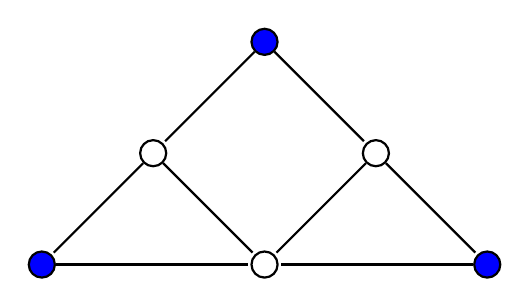
\begin{tikzpicture}[-,>=stealth,shorten >=1pt,auto,node distance=2cm,thick,main node/.style={scale=1,circle,draw,font=\sffamily\normalsize}]
            \node[main node] (1) [fill=blue]{};
            \node[main node] (2) [below left of=1] {};
            \node[main node] (3) [below right of=1] {};
            \node[main node] (4) [below right of=2] {};
            \node[main node] (5) [fill=blue, below left of=2] {};
            \node[main node] (6) [fill=blue, below right of=3] {};

            \path[every node/.style={font=\sffamily\small}]
                (1) edge (2)
                (1) edge (3)
                (2) edge (4)
                (3) edge (4)
                (2) edge (5)
                (3) edge (6)
                (5) edge (4)
                (6) edge (4)
                ;
        \end{tikzpicture}

        \textit{The blue nodes are the biggest possible independent set of the graph}
    \end{center}

    \begin{framedprob}{The Maximum-weight Independent Set problem}
        Given a vertex-weighted undirected graph $G$, meaning that the weights are on the vertices and not on the edges, find an independent set $X \subseteq V(G)$ such that the sum of the weights of the vertices in $X$ is maximal, meaning that:
        \[X = \argmax_{\substack{H \text{ independent}\\ \text{set of } G}} \rbk{\sum_{u \in H} w(u)}\]
    \end{framedprob}

    This problem can be easily reduced to a 0-1 integer program, that being an integer program where every variable is either a 0 or a 1:
    \begin{itemize}
        \item For every node $v \in V(G)$, we define the variabile $x_v$ and the constant $w_v$ such that $w_v = w(v)$. 
        \item For every edge $(i,j) \in E(G)$, we add the constraint $x_i + x_j \leq 1$. This constraint enforces that at most one between $x_i$ and $x_j$ can be set to 1.
    \end{itemize}

    We get that:
    \[\begin{array}{ccc}
        \qquad\qquad\quad
        & \max \; \sum\limits_{i = 1}^n w_i x_i \\\\
        & x_i + x_j \leq 1 & \forall (i,j) \in E(G) \\
        & x \in \{0,1\}^n
    \end{array}\]

    \textit{Note}: the constraint $x \in \{0,1\}$ is just a short-hand for the two constraints $0 \leq x \leq 1$ and $x \in \Z^n$, where $n = \abs{V(G)}$.

    By means of construction of this 0-1 integer program, \textbf{any feasible solution $\overline{x}$ corresponds to an independent set $X$} where $\overline{x_v} = 0 \iff v \notin X$. Due to this nature, we also use the term \textbf{indicator vector} to define feasible solutions. Any \textbf{optimal indicator vector} of this program corresponds to a maximum-weight independent set.
    
    However, the applied constraints are still to \textit{weak} since they exclude very few points from $\R^n$. As shown in the previous section, we can solve this program by repeatedly applying Gomory's Cutting Planes method. Nevertheless, before applying the procedure, we can manually find some constraints to our program find which we are sure to be true.

    For example, let $C \subseteq V(G)$ be a \textbf{clique} of $G$, i.e. a subset of vertices where $\forall x,y \in C \;\; (x,y) (y,x) \in (G)$. By the very own definition of clique, it's easy to see that the concepts of clique and independent set are \textit{complementary} to each other. Thus, there must be some constraint that we can apply on each clique of $G$ in order to remove them from the feasible region.

    Suppose our graph has a 3-clique made of the vertices $i,j,k \in V(G)$. Since they form a clique, we know that $(i,j), (j,k), (k,i) \in E(G)$. Thus, in our linear program we must have the three constraints $x_i+ x_j \leq 1$, $x_j+x_k \leq 1$ and $x_k + x_i \leq 1$. These three constraints can be summed to form the following linear combination:
    \[2x_i + 2x_j + 2x_k \leq 3 \implies x_1+x_j+x_k \leq \frac{3}{2}\]

    Since it's a linear combination of the three constraints, we know that this inequality is already implied by the very same three constraints. However, since $i,j,k$ form a clique, we know that if we add \textit{any} node between the three of them to our independent set then we cannot add any other of them. This condition can be easily described by adding the constraint $x_i + x_j + x_k \leq 1$ which can't be obtained as a linear combination of the previous three constraint, reducing the set of feasible region. In general, for each clique $C$ we can add the constraint $\sum\limits_{i \in V(C)} x_i \leq 1$ to pick maximum one member of the clique.

    In a similar way, we can enforce some constraints on the cycles of $G$: if $C'$ is an \textbf{odd cycle} of $G$ of length $2k+1$ then we can select at most $k$ nodes inside this cycle simply by skipping one node of the cycle for each selected node.

    After these observations, we can restate our 0-1 integer program as:
    \[\begin{array}{rrl}
        \qquad\qquad\qquad
        & \max \; \sum\limits_{i = 1}^n w_i x_i \\\\
        &x_i + x_j \leq 1  & \forall (i,j) \in E(G) \\
        &\sum\limits_{i \in V(C)} x_i \leq 1 & \forall \text{ cliques } C \text{ in } G \\
        &\sum\limits_{i \in V(C')} x_i \leq k & \forall \text{ cycles } C' \text{ of length } 2k+1 \text{ in } G \\
        & x \in \{0,1\}
    \end{array}\]

    Even thought, these constraints are good enough to remove a lot of solutions from the feasible region, finding a clique of arbitrary length in a graph is also an \textsf{NP}-Complete problem, so finding them would be as hard as solving the linear program. However, cliques with a fixed amount of vertices and all odd cycles can be found in polynomial time, meaning that we can still preserve some of these constraints.

    \quad

    \section{The Maximum-weight Perfect Matching problem}
    \label{perfect_match}

    \begin{frameddefn}{Matching}
        Let $G$ be an undirected graph. A subset $M \subseteq E(G)$ is said to be a \textbf{matching} if all the edges inside it have no common end-points, meaning that:
        \[\forall (u,v), (x,y) \in M\;\; u,v \neq x,y\] 

        A matching $M$ is said to be \textbf{perfect} if $V(M) = V(G)$, meaning that it covers all the vertices. Equivalently, a matching $M$ is perfect if $\abs{M} = \frac{\abs{V(G)}}{2}$.
    \end{frameddefn}

    \quad

    \begin{center}
        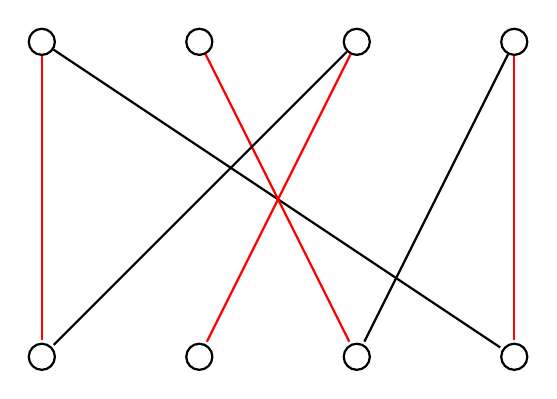
\begin{tikzpicture}[-,>=stealth,shorten >=1pt,auto,node distance=2cm,thick,main node/.style={scale=1,circle,draw,font=\sffamily\normalsize}]
            \node[main node] (1) []{};
            \node[main node] (2) [right of=1] {};
            \node[main node] (3) [right of=2] {};
            \node[main node] (4) [right of=3] {};
            \node (5) [below of=1] {};
            \node[main node] (6) [below of=5] {};
            \node[main node] (7) [right of=6] {};
            \node[main node] (8) [right of=7] {};
            \node[main node] (9) [right of=8] {};

            \path[every node/.style={font=\sffamily\small}]
                    (1) edge[color=red] (6)
                    (1) edge (9)
                    (2) edge[color=red] (8)
                    (3) edge (6)
                    (3) edge[color=red] (7)
                    (4) edge (8)
                    (4) edge[color=red] (9)
                ;
        \end{tikzpicture}

        \textit{The red edges are a perfect matching of the graph}
    \end{center}

    \begin{framedprob}{The Maximum-weight Perfect Matching problem}
        Given an edge-weighted undirected graph $G$, find a perfect matching $M \subseteq E(G)$ such that the sum of the weights of the edges in $M$ is maximal, meaning that:
        \[M = \argmax_{\substack{H \text{ perfect}\\ \text{matching of } G}} \rbk{\sum_{e \in H} w(e)}\]
    \end{framedprob}

    Just like the \textit{Maximum-weight Independent Set problem}, we can easily formulate the Maximum-weight Perfect Matching problem as a 0-1 integer program:
    \begin{itemize}
        \item For every edge $e \in E(G)$, we define the variabile $x_e$ and the constant $w_e$ such that $w_e = w(e)$. 
        \item For every vertex $v \in V(G)$ we add the constraint $\sum\limits_{e \in \delta(v)} x_e = 1$, where $\delta(v)$ is the set of edges with $v$ as one of the end-points, meaning that $\delta(v) = \{(x,y) \in E(G) \mid x = v \lor y = v\}$.
    \end{itemize}

    We get that:
    \[\begin{array}{ccc}
        \qquad\qquad\quad
        & \max \; \sum\limits_{e \in E(G)} w_e x_e \\\\
        & \sum\limits_{e \in \delta(v)} x_e = 1 & \forall v \in V(G) \\
        & x \in \{0,1\}^m
    \end{array}\]

    where $x_e = 0$ if and only if $e$ is not in the matching.

    \textbf{Note}: $m$ is the number of edges of $G$, i.e. $m = \abs{E(G)}$.

    We notice that the constraint added for each vertex already implies that for each edge $e$ it holds that $x_e \leq 1$.
    
    Thus, we can actually remove this constraint from our program.

    \[\begin{array}{ccc}
        \qquad\qquad\quad
        & \max \; \sum\limits_{e \in E(G)} w_e x_e \\\\
        & \sum\limits_{e \in \delta(v)} x_e = 1 & \forall v \in V(G) \\
        & x \geq 0 \\
        & x \in \Z^m
    \end{array}\]

    

    \newpage

    Consider now the \textbf{LP relaxation} of this integer program, that being the program identical to the original but without the integral constraint.

    \[\begin{array}{ccc}
        \qquad\qquad\quad
        & \max \; \sum\limits_{e \in E(G)} w_e x_e \\\\
        & \sum\limits_{e \in \delta(v)} x_e = 1 & \forall v \in V(G) \\
        & x \geq 0 \\
        & x \in \R^m
    \end{array}\]

    First, we notice that since we said that $x_e = 0$ if and only if $e$ is not in the matching, this implies that if $0 < x_e < 1$ the edge $e$ will be considered as an element of the subset, giving us the following observation.

    \begin{framedobs}{}
        Given a graph $G$, if $x$ is a \textbf{non-integral feasible solution} of the above linear program then the subset $M_x \subseteq E(G)$ represented by $x$ is \textbf{not a matching of $G$}.
    \end{framedobs}

    
    \proofenv{

        Let $v \in V(G)$ and suppose that $x \in P - \Z^m$. Due to the constraints of the linear program, we have that $\sum\limits_{e \in \delta(v)} x_e = 1$. Thus, since $x$ is non-integral, there must at least two edges adjacent to $v$ whose indicator variable is different from 0 in order to reach sum 1.
        
        Thus, at least two edges adjacent to $v$ are in the subset $M \subseteq E(G)$ represented by $x$. However, by definition of matching, this also implies that $M$ is not a matching.
    }

    \begin{framedlem}[label=int_iff_pm]{}
        Given a graph $G$, any feasible solution $x$ of the linear program above is \textbf{integral if and only if $M_x$ is a perfect matching} of the graph $G$.
    \end{framedlem}

    \proofenv{

        If $x$ is non-integral by the previous observation we know that $M_x$ isn't a matching. Vice versa, if $x$ is integral then for each node $v \in V(G)$ only one edge adjacent to $v$ will be in $M_x$, concluding that $M_x$ is a perfect matching of $G$. 
    }

    \begin{frameddefn}{Convex hull of the perfect matchings}
        Given a graph $G$, we define $P_M(G)$ as the \textbf{convex hull} of all the indicator vertices $v_1, \ldots, v_k$ representing the \textbf{perfect matchings of $G$}.
    \end{frameddefn}

    \begin{framedcor}[label=P_M(G)_in_P]{}
        Let $G$ be a weighted graph and let $P$ be the polyhedron given by the LP relaxation shown above. Then, it holds that $P_M(G) \subseteq P$.
    \end{framedcor}

    \proofenv{

        All the vertices $\overline{x_{1}}, \ldots, \overline{x_{k}}$ of $P_M(G)$ describe a perfect matching of $G$. Thus, by \cref{int_iff_pm} we know that they must be integral feasible solutions of the LP relaxation, meaning that $\overline{x_{1}}, \ldots, \overline{x_{k}} \in P$. Then, since $P_M(G)$ is by definition the convex combination of $\overline{x_{1}}, \ldots, \overline{x_{k}}$, for any point $x \in P_M(G)$ it must also hold that $x \in P$.
    }

    We will show that, if some conditions are met, the LP relaxation of this program has \textbf{only integral vertices}, meaning that all of them correspond to a maximum weight perfect matching.

    \quad

    \subsection{The Max PM problem for bipartite graphs}

    \begin{frameddefn}{Bipartite graph}
        An undirected graph $G$ is said to be a \textbf{bipartite graph} if it can be partitioned into two independent sets $X,Y$. Equivalently, $G$ is bipartite if there are two sets $X,Y$ such that for every edge $(x,y) \in E(G)$ it holds that $x \in X$ and $y \in Y$ (or vice versa).
    \end{frameddefn}

    \begin{center}
        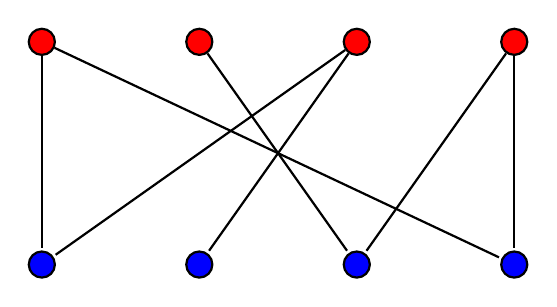
\begin{tikzpicture}[-,>=stealth,shorten >=1pt,auto,node distance=2cm,thick,main node/.style={scale=1,circle,draw,font=\sffamily\normalsize}]
            \node[main node] (1) [fill=red,]{};
            \node[main node] (2) [fill=red,right of=1] {};
            \node[main node] (3) [fill=red,right of=2] {};
            \node[main node] (4) [fill=red,right of=3] {};
            \node (5) [below right of=1] {};
            \node[main node] (6) [fill=blue,below left of=5] {};
            \node[main node] (7) [fill=blue,right of=6] {};
            \node[main node] (8) [fill=blue,right of=7] {};
            \node[main node] (9) [fill=blue,right of=8] {};

            \path[every node/.style={font=\sffamily\small}]
                    (1) edge (6)
                    (1) edge (9)
                    (2) edge (8)
                    (3) edge (6)
                    (3) edge (7)
                    (4) edge (8)
                    (4) edge (9)
                ;
        \end{tikzpicture}

        \textit{The red and blue nodes partition the graph into two independent sets}
    \end{center}

    \begin{framedprop}[label=bipartite_no_odd_cycles]{}
        A graph $G$ is \textbf{bipartite} if and only if it has \textbf{no odd cycles}.

        \textit{(proof omitted)}
    \end{framedprop}

    \begin{framedprop}[label=cyclic_deg_2]{}
        If $G$ is an undirected graph where all nodes have degree at least 2, then $G$ is \textbf{cyclic}.

        \textit{(proof omitted)}
    \end{framedprop}

    \begin{framedthm}[label=max_pm_bipartite]{Max-weight PM in bipartite graphs}
        Let $G$ be a bipartite weighted graph and let $P$ be the polyhedron defined as:
        \[P = \cbk{x \in \R^m \left | x \geq 0, \sum\limits_{e \in \delta(v)} x_e = 1 \;\; \forall v \in V(G) \right .}\]

        Every vertex $\overline{x} \in P$ is \textbf{integral}, meaning that $\overline{x} \in \Z^m$.
    \end{framedthm}
    
    \proofenv{

        Let $\overline{x} \in P$ be a vertex of $P$. By way of contradiction, suppose that $\overline{x} \notin \Z^m$ and let $\mathcal{U} = \{e \in E(G) \mid 0 < \overline{x_e} < 1\}$. Since we assumed that $\overline{x} \notin \Z^m$, it must hold that $\mathcal{U} \neq \varnothing$. Let $G_\mathcal{U}$ be the subgraph of $G$ made of the edges in $\mathcal{U}$.

        \textbf{Claim}: Every vertex in $V(G_\mathcal{U})$ has degree at least 2

        \proofenv[Proof of the claim]{

            For each vertex $v \in V(G_\mathcal{U})$, it holds that $\mathcal{U} \cap \delta(v) \neq \varnothing$. By way of contradiction, suppose that $\exists e \in \delta(v)$ such that $\overline{x_e} = 1$. Then, we get that:
            \[\sum_{f \in \delta(v)} \overline{x_f} = 1 \implies \sum_{f \in \delta(v)-\{e\}} \overline{x_f} = 1 - \overline{x_e} = 0 \implies \forall f \in \delta(v)-\{e\} \;\; \overline{x_f} = 0\]

            Since $x_e = 1$ and $\forall f \in \delta(v)-\{e\} \;\; \overline{x_f} = 0$, we derive that $\mathcal{U} \cap \delta(v) = \varnothing$, which is absurd. Thus, $\forall e \in \delta(v)$ it must hold that $\overline{x_e} < 1$, implying that in order for $\overline{x}$ to respect the constraints there must be one or more edges $e_1, \ldots, e_k \in (\mathcal{U} \cap \delta(v))-\{e\}$ such that $x_e + \sum_{i = 1}^k \overline{x_{e_i}} = 1$, meaning that $\abs{\delta(v)} \geq 2$.
        }

        Since $G_\mathcal{U}$ is undirected and all its nodes have degree at least 2, by \cref{cyclic_deg_2} there must be a cycle $C \subseteq G_\mathcal{U} \subseteq G$. Moreover, since $G$ is bipartite, by \cref{bipartite_no_odd_cycles} this cycle $C$ must be an even cycle of length $2k$ for some $k \in \N$.

        Let $e_1, \ldots, e_{2k}$ be the edges of $C$. Let $\varepsilon = \min_{i = 1}^k (\min (x_{e_i}, 1-x_{e_i}))$, meaning that $\varepsilon$ is the minimal possible value such that there is a variabile between $x_{e_1}, \ldots, x_{e_{2_k}}$ for which it holds either that $x_{e_i} + \varepsilon = 1$ or that $x_{e_i} - \varepsilon = 0$.

        Let $y$ and $y'$ be two indicator vectors defined as:
        \[y_{e} = \left \{ \begin{array}{ll}
            \overline{x_{e}} - \varepsilon & \text{ if $e = e_i$ for some $1 \leq i \leq 2k$ and $i$ is even}\\
            \overline{x_{e}} + \varepsilon & \text{ if $e = e_i$ for some $1 \leq i \leq 2k$ and $i$ is odd}\\
            \overline{x_{e}} & \text{ otherwise}
        \end{array}\right . \]

        \[y_{e}' = \left \{ \begin{array}{ll}
            \overline{x_{e}} + \varepsilon & \text{ if $e = e_i$ for some $1 \leq i \leq 2k$ and $i$ is even}\\
            \overline{x_{e}} - \varepsilon & \text{ if $e = e_i$ for some $1 \leq i \leq 2k$ and $i$ is odd}\\
            \overline{x_{e}} & \text{ otherwise}
        \end{array}\right . \]
    

        In other words, $y$ is the indicator vector obtained by adding $\varepsilon$ to all even edges of the cycle $C$ and subtracting $\varepsilon$ to all the odd edges, while $y'$ is the indicator vector obtained by doing the inverse.

        \begin{figure}[H]
            \centering

            \begin{tabular}{ccc}
                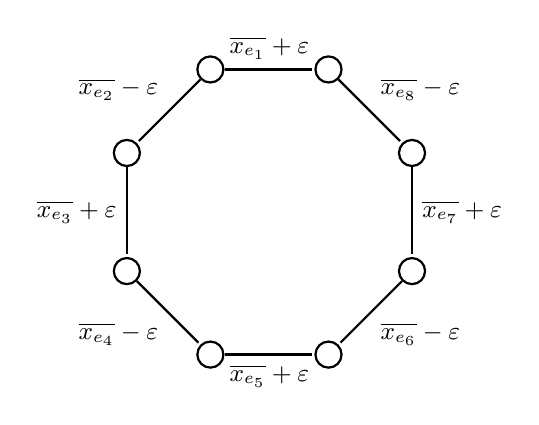
\begin{tikzpicture}[-,>=stealth,shorten >=1pt,auto,node distance=1.5cm,thick,main node/.style={scale=1,circle,draw,font=\sffamily\normalsize}]
                    \node[main node] (1) []{};
                    \node[main node] (2) [right of = 1]{};

                    \node[main node] (3) [below left of = 1]{};
                    \node[main node] (4) [below of = 3]{};
                    \node[main node] (5) [below right of = 4]{};

                    \node[main node] (6) [below right of = 2]{};
                    \node[main node] (7) [below of = 6]{};
                    \node[main node] (8) [below left of = 7]{};

                    \path[every node/.style={font=\sffamily\small}]
                            (1) edge [] node {$\overline{x_{e_1}} + \varepsilon$} (2)

                            (1) edge [swap] node {$\overline{x_{e_2}} - \varepsilon$} (3)
                            (3) edge [swap] node {$\overline{x_{e_3}} + \varepsilon$} (4)
                            (4) edge [swap] node {$\overline{x_{e_4}} - \varepsilon$} (5)
                            
                            (2) edge [] node {$\overline{x_{e_8}} - \varepsilon$} (6)
                            (6) edge [] node {$\overline{x_{e_7}} + \varepsilon$} (7)
                            (7) edge [] node {$\overline{x_{e_6}} - \varepsilon$} (8)

                            (5) edge [swap] node {$\overline{x_{e_5}} + \varepsilon$} (8)
                        ;
                \end{tikzpicture}

                &\qquad\qquad&

                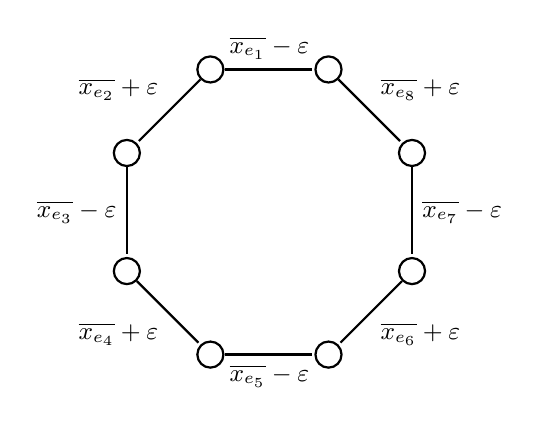
\begin{tikzpicture}[-,>=stealth,shorten >=1pt,auto,node distance=1.5cm,thick,main node/.style={scale=1,circle,draw,font=\sffamily\normalsize}]
                    \node[main node] (1) []{};
                    \node[main node] (2) [right of = 1]{};

                    \node[main node] (3) [below left of = 1]{};
                    \node[main node] (4) [below of = 3]{};
                    \node[main node] (5) [below right of = 4]{};

                    \node[main node] (6) [below right of = 2]{};
                    \node[main node] (7) [below of = 6]{};
                    \node[main node] (8) [below left of = 7]{};

                    \path[every node/.style={font=\sffamily\small}]
                            (1) edge [] node {$\overline{x_{e_1}} - \varepsilon$} (2)

                            (1) edge [swap] node {$\overline{x_{e_2}} + \varepsilon$} (3)
                            (3) edge [swap] node {$\overline{x_{e_3}} - \varepsilon$} (4)
                            (4) edge [swap] node {$\overline{x_{e_4}} + \varepsilon$} (5)
                            
                            (2) edge [] node {$\overline{x_{e_8}} + \varepsilon$} (6)
                            (6) edge [] node {$\overline{x_{e_7}} - \varepsilon$} (7)
                            (7) edge [] node {$\overline{x_{e_6}} + \varepsilon$} (8)

                            (5) edge [swap] node {$\overline{x_{e_5}} - \varepsilon$} (8)
                        ;
                \end{tikzpicture}
            \end{tabular}

            \caption{The vector $y$ is shown on the left, $y'$ on the right}
        \end{figure}
        
        Since the cycle has an even amount of edges, the value $\varepsilon$ gets added and subtracted an equal amount of times, so we get that for each node $v \in V(C)$ the constraint $\sum_{e \in \delta(v)} x_e = 1$ is still satisfied. Moreover, by choice of $\varepsilon$, we are sure that $0 \leq y,y' \leq 1$ holds, so every constraint is still satisfied by both $y$ an $y'$, meaning that they are indeed feasible solutions and thus that $y,y' \in P$.

        In particular, the way $y$ and $y'$ are defined also implies that:
        \[\sum_{e \in E(G)} \overline{x_e} = \sum_{e \in E(G)} x_e = \sum_{e \in E(G)} y'_e\]
        meaning that $\overline{x} = \frac{1}{2}y + \frac{1}{2}y'$.
        Now, since $\overline{x}$ is a vertex of $P$, by definition there is an affine hyperplane $H$ such that $H = \{x \in \R^m \mid c^Tx = c^T\overline{x}\}$, $\{x\} = P \cap H$ and $\forall z \in P-\{x\} \;\; c^Tz < c^T\overline{x}$.

        By linearity, we notice that:
        \[\overline{x} = \frac{1}{2}y + \frac{1}{2}y' \implies c^T\overline{x} = \frac{1}{2}c^Ty + \frac{1}{2}c^Ty'\]

        Thus, it must hold either that $c^T\overline{x} = c^Ty + c^Ty'$, which is a contradiction to the fact that $\{x\} = P \cap H$, or that $c^Ty > c^T\overline{x} \lor c^Ty' > c^T\overline{x}$, which is a contradiction to the fact that $\forall z \in P-\{x\} \;\; c^Tz < c^T\overline{x}$.
        
        In other words, $\overline{x} = \frac{1}{2}y + \frac{1}{2}y'$ implies that $\overline{x}$ is inside the segment from $y$ to $y'$, which means that this segment must either lie of the hyperplane $H$ or pierce through it, which in both cases is a contradiction to the fact that $\overline{x}$ is a vertex of $P$. Thus, the only possibility is that $\overline{x} \in \Z^m$ must hold.

    }

    \newpage

    \begin{framedcor}{}
        Let $G$ be a weighted graph and let $P$ be the polyhedron given by the LP relaxation shown above. If $G$ is \textbf{bipartite} then $P = P_M(G)$.

        \textbf{Note}: this result is not equal to saying that $P = P_I$.
    \end{framedcor}

    \proofenv{
        By \cref{P_M(G)_in_P}, we know that $P_M(G) \subseteq P$. Moreover, by \cref{max_pm_bipartite} we know that all the vertices $\overline{x_{1}}, \ldots, \overline{x_{k}}$ of $P$ are integral. Thus, by \cref{int_iff_pm} we know that they must describe perfect matchings of $G$, meaning that $\overline{x_{1}}, \ldots, \overline{x_{k}} \in P_(G)$. Then, since $P$ is the convex combination of $\overline{x_{1}}, \ldots, \overline{x_{k}}$, for any point $x \in P$ it must also hold that $x \in P_M(G)$.
    }

    This result shows that if the graph is \textbf{bipartite} than we find an optimal integral solution simply by solving the LP relaxation, making this integer program theoretically \textbf{solvable in polynomial time} (in case of bipartite graphs). In fact, many other algorithms can solve this problem efficiently without the need of integer programming at all (this problem isn't \textsf{NP}-Complete, so this doesn't get us to anything).


    \quad

    \subsection{The Max PM problem for non-bipartite graphs}

    What can we do if the graph isn't bipartite? With only the previous constraints, some non-bipartite graphs can be formulated in a way such that there can be non-integral vertices in the polyhedron, meaning that the previous theorem doesn't hold. Nevertheless, we can add some more constraints to the problem in order to get an \textbf{even stronger result} than the one previously shown.

    First, we define an extension of the function $\delta$: if $W \subseteq V(G)$ then $\delta(W) = \{(u,v) \in E(G) \mid u \in W, v \in V(G)- W\}$, i.e. the set of edges exiting $W$. Now, we restate the 0-1 integer program with the following new constraint: 
    
    \[\begin{array}{crl}
        \qquad\qquad\qquad\qquad
        & \max \; \sum\limits_{e \in E(G)} w_e x_e \\\\
        & \sum\limits_{e \in \delta(v)} x_e = 1 & \forall v \in V(G) \\
        & \sum\limits_{e \in \delta(\mathcal{U})} x_e \geq 1 & \forall\, \mathcal{U} \subseteq V(G) \text{ s.t  } \abs{\mathcal{U}} = 2k+1 \\
        & x \in \{0,1\}^m
    \end{array}\]

    As before, the LP relaxation can be obtained by substituting the constraint $x \in \{0,1\}^m$ with the constraints $x \geq 0$ and $x \in \R^m$. Moreover, \cref{int_iff_pm} holds even in this LP relaxation.

    \begin{framedthm}[label=max_pm_non_bipartite]{Edmond's theorem for general Max-weight PM}
        Let $G$ be a weighted graph and let $P$ be the polyhedron given by the LP relaxation shown above. Then, it holds that $P = P_M(G)$.
    \end{framedthm}

    \proofenv{

        First, we notice that for each graph that has an odd number of nodes there cannot be a perfect matching and the polyhedron of the linear program has no feasible solution, meaning that $P_M(G) = \varnothing = P_M(G)$.
        
        Hence, for the proof we consider only graphs with an odd number of nodes. By \cref{P_M(G)_in_P}, we already know that $P_M(G') \subseteq P$ holds for all such graphs.

        By way of contradiction, suppose that there are some counterexamples such that $P_M(G') \neq P$ holds. Let $G$ be the counterexample with the least amount of nodes such that $P_M(G) \neq P$. Since $P$ is bounded and $P_M(G)$ is a proper subset of $P$, there must be at least a vertex $\overline{x}$ of $P$ that is outside of $P_M(G)$.
        
        Since by definition $P_M(G)$ is the convex hull of all the perfect matchings of $G$ and $\overline{x}$ isn't a vertex of $P_M(G)$, we know that it also isn't a perfect matching. Thus, by \cref{int_iff_pm} we know that $\overline{x} \notin \Z^m$ and let $\mathcal{U} \subseteq V(G)$ be a subset such that $\abs{\mathcal{U}} = 2k+1$ for some $k \in \N$
        
        \begin{enumerate}
            \item[Case 1.] Suppose that $\sum\limits_{e \in \delta(\mathcal{U})} x_e > 1$.

            Let $\mathcal{F} = \{e \in E(G) \mid 0 < \overline{x_e} < 1\}$. Since we assumed that $\overline{x} \notin \Z^m$, it must hold that $\mathcal{F} \neq \varnothing$. Let $G_\mathcal{F}$ be the subgraph of $G$ made of the edges in $\mathcal{F}$.

            \textbf{Claim 1}: Every node in $V(G_\mathcal{F})$ has degree at least 2

            \proofenv[Proof of the claim]{
                Under the assumption that $\sum\limits_{e \in \delta(\mathcal{U})} x_e > 1$ holds, the proof of this claim is equivalent to the one seen for the bipartite case of this theorem (see \cref{max_pm_bipartite}).
            }
            
            \textbf{Claim 2}: $G_\mathcal{F}$ has no even length cycle

            \proofenv[Proof of the claim]{
                
                By way of contradiction, suppose there is a cycle $C$ of even length in $G_\mathcal{F}$ and let $e_1, \ldots, e_{2k}$ be the edges of $C$. Let $\varepsilon = \min\limits_{\substack{X \subseteq V(G), \\ \abs{X} \text{ odd}}} \rbk{\sum\limits_{e \in \delta(X)} \frac{\overline{x_e} -1}{\abs{V(G)}}}$.
        
                Let $y$ and $y'$ be two indicator vectors defined as:
                \[y_{e} = \left \{ \begin{array}{ll}
                    \overline{x_{e}} - \varepsilon & \text{ if $e = e_i$ for some $1 \leq i \leq 2k$ and $i$ is even}\\
                    \overline{x_{e}} + \varepsilon & \text{ if $e = e_i$ for some $1 \leq i \leq 2k$ and $i$ is odd}\\
                    \overline{x_{e}} & \text{ otherwise}
                \end{array}\right . \]
        
                \[y_{e}' = \left \{ \begin{array}{ll}
                    \overline{x_{e}} + \varepsilon & \text{ if $e = e_i$ for some $1 \leq i \leq 2k$ and $i$ is even}\\
                    \overline{x_{e}} - \varepsilon & \text{ if $e = e_i$ for some $1 \leq i \leq 2k$ and $i$ is odd}\\
                    \overline{x_{e}} & \text{ otherwise}
                \end{array}\right . \]
                
                Just like in the bipartite case of this theorem (see \cref{max_pm_bipartite}), by choice of $\varepsilon$ we get that $y,y' \in P$ and that $\overline{x} = \frac{1}{2} y + \frac{1}{2} y'$, which is absurd since $\overline{x}$ is assumed to be a vertex of $P$. Thus, such even cycle cannot exist.

            }

            Since $G_{\mathcal{F}}$ has no odd cycle and all of its nodes have degree at least 2, by \cref{cyclic_deg_2} there must be an odd cycle $C \subseteq G_\mathcal{F} \subseteq G$ of length $2k +1$ for some $k \in \N$. Let $v_1, \ldots, v_{2k+1}$ be the nodes of such cycle $C$.

            \textbf{Claim 3}: For all $i \neq j$ such that $i \neq 1, j \neq 2k+1$ and $\abs{i-j} > 1$, the nodes $v_i$ and $v_j$ are no adjacent to each other

            \proofenv[Proof of the claim]{

                By way of contradiction, suppose the claim is false for some indices $i,j$. Then, the edge $(v_i, v_j)$ would split the odd cycle $C$ into two subcycles $C_1, C_2$ where one of them is an even cycle and the other is odd. However, we said that $G_{\mathcal{F}}$ has no even length cycle, raising a contradiction.

                \begin{figure}[H]
                    \centering
                    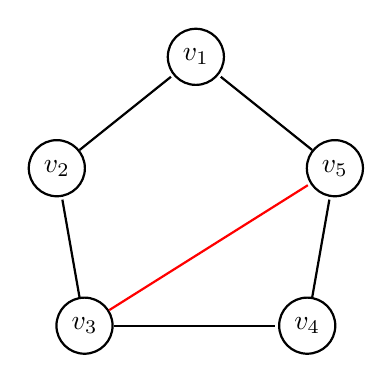
\begin{tikzpicture}[-,>=stealth,shorten >=1pt,auto,node distance=2cm,thick,main node/.style={scale=1,circle,draw,font=\sffamily\normalsize}]
                        \node[] (1) []{};
                        \node[main node] (2) [below left of = 1]{$v_3$};
                        \node[main node] (3) [below right of = 1]{$v_4$};

                        \node[main node] (4) [above of = 2, xshift = -10]{$v_2$};
                        \node[main node] (5) [above of = 3, xshift =  10]{$v_5$};

                        \node[main node] (6) [above of = 1]{$v_1$};

                        \path[every node/.style={font=\sffamily\small}]
                                (2) edge  (3)
                                (2) edge  (4)
                                (3) edge  (5)
                                
                                (4) edge  (6)
                                (5) edge  (6)

                                (2) edge [color=red]  (5)
                            ;
                    \end{tikzpicture}

                    \caption{The edge $(v_3, v_5)$ would split the cycle in an odd subcycle and an even subcycle}
                \end{figure}
            }

            \textbf{Claim 4}: There is at least a node $v_i$ in $C$ with a neighbor $u \in V(G_\mathcal{F})$ such that $u \notin V(C)$.
            
            \proofenv[Proof of the claim]{
                
                Since $\abs{C}$ is odd, by the constraints of the linear program we know that $\sum\limits_{e \in \delta(V(C))} \overline{x_e} \geq 1$. However, we know that there is no edge $f$ in $C$ such that $x_f = 1$ and $v_i$ is one of the two ends of $f$ since this would imply that $\sum\limits_{g \in \delta(v)} \overline{x_g} > 1$, violating the latter constraint. Thus, thanks to the previous claim, in order for the first constraint to hold without breaking the second one, there must be an edge $e$ incident to $v_i$ that is not in $C$. 
            }

            Since we know that there is a node that touches the cycle $C$, let $w_1, \ldots, w_t$ be a walk such that:
            \begin{itemize}
                \item $w_1 = v_i$
                \item $w_1, \ldots, w_{t-1}$ are all distinct
                \item $w_2, \ldots, w_{t-1}$ are not in $C$
                \item $t$ is the maximal possible index
            \end{itemize}

            In other words, the walk $w_1, \ldots, w_t$ is the longest possible walk going outside of the cycle $C$. Since every node $G_\mathcal{F}$ has degree at least 2 and $t$ is chosen as maximal, it must hold that the walk either cycles back on itself or that it cycles back to $C$, i.e. it holds that $w_t = w_h$ where $1 \leq h \leq t-1$ or that $w_t = v_j$ where $i \leq j \leq 2k+1$. In both cases, we notice that the cycle formed must be of odd length since there can be no even length cycle in $G_\mathcal{F}$.

            \textbf{Claim 5}: For all $\ell \neq j$ it holds that $w_\ell \neq v_j$

            \proofenv[Proof of the claim]{

                By way of contradiction, suppose that there are some indices $i \neq j$ such that $w_\ell = v_j$, meaning that $v_i, w_2, \ldots, w_\ell, v_{j+1}, \ldots, v_{2k+1}, v_1, \ldots, v_i$ forms a cycle $C'$. Since $G_\mathcal{F}$ can only have odd length cycles.
                
                Then, $v_1, \ldots, v_{i-1}, v_i, w_2, \ldots, w_\ell, v_{j+1}, \ldots, v_{2k}, v_1$ would make a cycle $C''$ of even length since it is the union of two odd length cycles where the common edges were excluded from both. However, such cycle can't exist in $G_\mathcal{F}$, raising a contradiction.

                \begin{figure}[H]
                    \centering
                    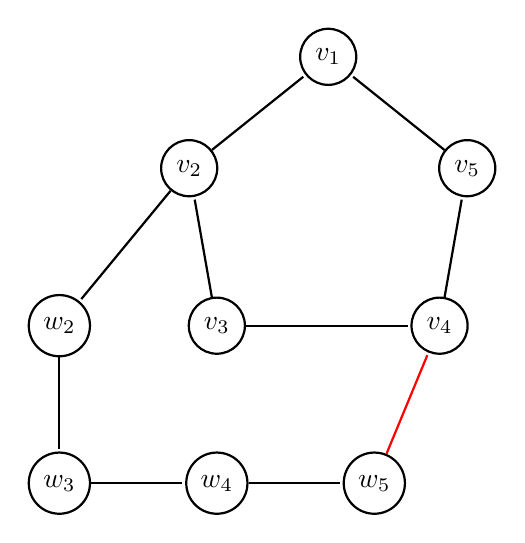
\begin{tikzpicture}[-,>=stealth,shorten >=1pt,auto,node distance=2cm,thick,main node/.style={scale=1,circle,draw,font=\sffamily\normalsize}]
                        \node[] (1) []{};
                        \node[main node] (2) [below left of = 1]{$v_3$};
                        \node[main node] (3) [below right of = 1]{$v_4$};

                        \node[main node] (4) [above of = 2, xshift = -10]{$v_2$};
                        \node[main node] (5) [above of = 3, xshift =  10]{$v_5$};

                        \node[main node] (6) [above of = 1]{$v_1$};

                        \node[main node] (7) [left of = 2]{$w_2$};
                        \node[main node] (8) [below of = 7]{$w_3$};
                        \node[main node] (9) [right of = 8]{$w_4$};
                        \node[main node] (10) [right of = 9]{$w_5$};

                        \path[every node/.style={font=\sffamily\small}]
                                (2) edge  (3)
                                (2) edge  (4)
                                (3) edge  (5)
                                
                                (4) edge  (6)
                                (5) edge  (6)

                                (4) edge (7)
                                (7) edge (8)
                                (8) edge (9)
                                (9) edge (10)
                                (10) edge[color=red] (3)

                            ;
                    \end{tikzpicture}

                    \caption{If $w_6 = v_4$ were to be true, $v_1, v_2, w_2, w_3, w_4, v_4, v_5, v_1$ would form an even cycle}
                \end{figure}
                
            }

            Due to the last claim, it must hold that the walk cycles back on itself, i.e. it holds that $w_t = w_h$ where $1 \leq h \leq t-1$. Let $C'$ be the cycle $w_h, \ldots, w_{t-1}, w_h$. The current setup is given by two disjoint odd length cycles $C$ and $C'$ connected by the path $w_1, \ldots, w_h$.

            Let $e_1, \ldots, e_{2k+1}$ be the edges of $C$, $f_1, \ldots, f_2r+1$ be the edges of $C'$ and $g_1, \ldots, g_{s}$ be the edges of the path $P = w_1, \ldots, w_h$
            
            Moreover, let $\varepsilon = \min\limits_{\substack{X \subseteq V(G), \\ \abs{X} \text{ odd}}} \rbk{\sum\limits_{e \in \delta(X)} \frac{\overline{x_e} -1}{\abs{V(G)}}}$.

            Like in \cref{max_pm_bipartite}, we consider the following two indicator vectors $z$ and $z'$ obtained through $\overline{x}$ where the value $\varepsilon$ (or $\frac{\varepsilon}{2}$ when needed) gets added/subtracted on even index edges and subtracted/added on odd index edges of $C, C'$ and $P$. The "distribution" must equal, i.e. the total sum of the addition and subtractions equals 0 and such that $\overline{x} = \frac{1}{2} z + \frac{1}{2} z'$.

            \begin{figure}[H]
                \centering
                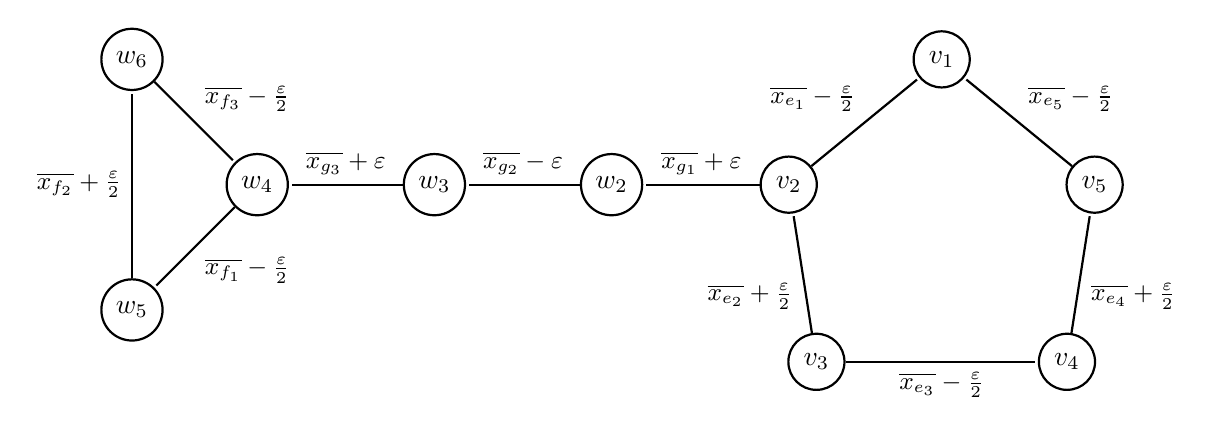
\begin{tikzpicture}[-,>=stealth,shorten >=1pt,auto,node distance=2.25cm,thick,main node/.style={scale=1,circle,draw,font=\sffamily\normalsize}]
                    \node[] (1) []{};
                    \node[main node] (2) [below left of = 1]{$v_3$};
                    \node[main node] (3) [below right of = 1]{$v_4$};

                    \node[main node] (4) [above of = 2, xshift = -10]{$v_2$};
                    \node[main node] (5) [above of = 3, xshift =  10]{$v_5$};

                    \node[main node] (6) [above of = 1]{$v_1$};

                    \node[main node] (7) [left of = 4]{$w_2$};
                    \node[main node] (8) [left of = 7]{$w_3$};
                    \node[main node] (9) [left of = 8]{$w_4$};
                    \node[main node] (10) [below left of = 9]{$w_5$};
                    \node[main node] (11) [above left of = 9]{$w_6$};

                    \path[every node/.style={font=\sffamily\small}]
                        (2) edge[swap] node{$\overline{x_{e_3}} - \frac{\varepsilon}{2}$}  (3)
                        (2) edge node{$\overline{x_{e_2}} + \frac{\varepsilon}{2}$}  (4)
                        (3) edge[swap] node{$\overline{x_{e_4}} + \frac{\varepsilon}{2}$}  (5)
                        
                        (4) edge node{$\overline{x_{e_1}} - \frac{\varepsilon}{2}$}  (6)
                        (5) edge[swap] node{$\overline{x_{e_5}} - \frac{\varepsilon}{2}$}  (6)

                        (4) edge[swap] node{$\overline{x_{g_1}} + \varepsilon$} (7)
                        (7) edge[swap] node{$\overline{x_{g_2}} - \varepsilon$} (8)
                        (8) edge[swap] node{$\overline{x_{g_3}} + \varepsilon$} (9)
                        
                        (9) edge node{$\overline{x_{f_1}} - \frac{\varepsilon}{2}$} (10)
                        (10) edge node{$\overline{x_{f_2}} + \frac{\varepsilon}{2}$} (11)
                        (11) edge node{$\overline{x_{f_3}} - \frac{\varepsilon}{2}$} (9)
                        ;
                \end{tikzpicture}
                \caption{Example of equal distribution on the vector $z$. The vector $z'$ would have all increments and decrements reversed.}
            \end{figure}

            Since such distribution can always be found and it doesn't violate the constraints, we get that $z,z' \in P$. Moreover, the segment from $z$ and $z'$ always lies on the hyperplane of the vertex $\overline{x}$ or pierces through it, which is absurd. Finally, due to all possibilities raising a contradiction in this case, it must hold that $P_M(G) = P$ when $\sum\limits_{e \in \delta(\mathcal{U})} \overline{x_e} > 1$.

        \item[Case 2.]  Suppose that $\sum\limits_{e \in \delta(\mathcal{U})} \overline{x_e} = 1$.
        
            Let $\overline{\mathcal{U}} = V(G) - \mathcal{U}$. Since we assumed that $\abs{V(G)}$ is even and $\abs{\mathcal{U}}$ is odd, it must also hold that $\overline{\mathcal{U}}$ is odd. Moreover, we notice that:
            \[\sum\limits_{e \in \delta(\overline{\mathcal{U}})} \overline{x_e} = \sum\limits_{e \in \delta(\mathcal{U})} \overline{x_e} = 1\]
            since $\delta(\overline{\mathcal{U}}) = \delta(\mathcal{U})$ by definition.

            We notice that in order for the constraint of this case to be tight it must hold that each value $x_e$ involved is rational, meaning that $\delta(\mathcal{U}) \subseteq \Q$. Otherwise, if one of them were irrational, there would be a little gap which cannot be filled.

            \begin{figure}[H]
                \centering
                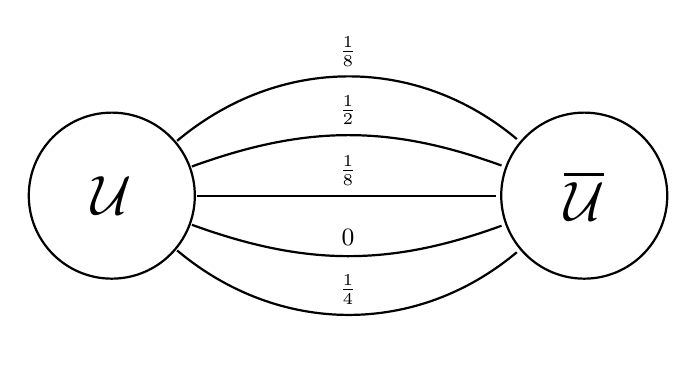
\begin{tikzpicture}[-,>=stealth,shorten >=1pt,auto,node distance=3cm,thick,main node/.style={scale=1,circle,draw,font=\sffamily\normalsize}]
                    \node[circle, draw=black, inner sep=0pt, minimum size=30pt, scale=2] (1) {$\mathcal{U}$};
                    \node[circle, draw=black, inner sep=0pt, minimum size=30pt, scale=2] (2) [right of = 1] {$\overline{\mathcal{U}}$};

                    \path[every node/.style={font=\sffamily\small}]
                        (1) edge[bend left = 40] node {$\frac{1}{8}$}(2)
                        (1) edge[bend left = 20] node {$\frac{1}{2}$}(2)
                        (1) edge node {$\frac{1}{8}$}(2)
                        (1) edge[bend right = 20]node {$0$}(2)
                        (1) edge[bend right = 40]node {$\frac{1}{4}$}(2)
                        ;
                \end{tikzpicture}
            \end{figure}

            Let $G_1$ be the graph obtained by collapsing $\mathcal{U}$ in a single node $w_1$ and let $x'$ be the copy of $\overline{x}$ for $G_1$. Likewise, let $G_2$ be the graph obtained by collapsing $\overline{\mathcal{U}}$ in a single node $w_2$ and let $x''$ be the copy of $\overline{x}$ for $G_2$.

            \begin{figure}[H]
                \centering
                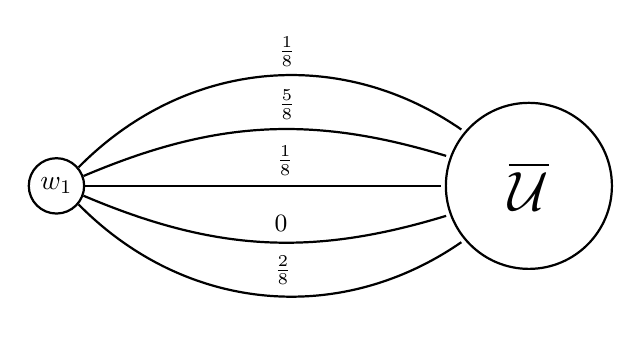
\begin{tikzpicture}[-,>=stealth,shorten >=1pt,auto,node distance=3cm,thick,main node/.style={scale=1,circle,draw,font=\sffamily\normalsize}]
                    \node[circle, draw=black, inner sep=0pt, minimum size=20pt] (1) {$w_1$};
                    \node[circle, draw=black, inner sep=0pt, minimum size=30pt, scale=2] (2) [right of = 1] {$\overline{\mathcal{U}}$};

                    \path[every node/.style={font=\sffamily\small}]
                        (1) edge[bend left = 40] node [xshift=15]{$\frac{1}{8}$}(2)
                        (1) edge[bend left = 20] node [xshift=15]{$\frac{5}{8}$}(2)
                        (1) edge node [xshift=7.5]{$\frac{1}{8}$}(2)
                        (1) edge[bend right = 20]node {$0$}(2)
                        (1) edge[bend right = 40]node {$\frac{2}{8}$}(2)
                        ;
                \end{tikzpicture}

                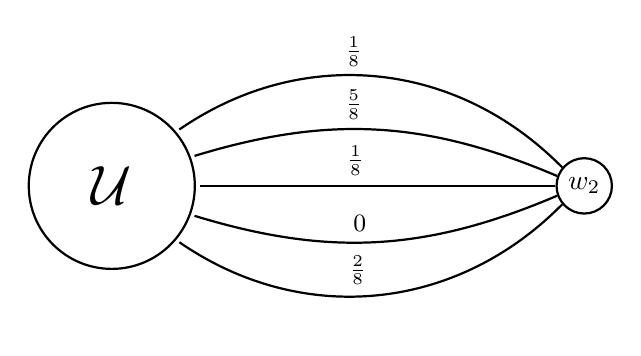
\begin{tikzpicture}[-,>=stealth,shorten >=1pt,auto,node distance=3cm,thick,main node/.style={scale=1,circle,draw,font=\sffamily\normalsize}]
                    \node[circle, draw=black, inner sep=0pt, minimum size=20pt] (1) {$w_2$};
                    \node[circle, draw=black, inner sep=0pt, minimum size=30pt, scale=2] (2) [left of = 1] {$\mathcal{U}$};

                    \path[every node/.style={font=\sffamily\small}]
                        (1) edge[swap, bend right = 40] node[xshift=-15]{$\frac{1}{8}$}(2)
                        (1) edge[swap, bend right = 20] node[xshift=-15]{$\frac{5}{8}$}(2)
                        (1) edge[swap] node [xshift=-7.5]{$\frac{1}{8}$}(2)
                        (1) edge[swap, bend left = 20]node {$0$}(2)
                        (1) edge[swap, bend left = 40]node {$\frac{2}{8}$}(2)
                        ;
                \end{tikzpicture}

                \caption{$G_1$ is shown above, $G_2$ is shown below}
            \end{figure}

            Since $\sum\limits_{e \in \delta(\mathcal{U})} x_e = 1$ holds by hypothesis, in $G_1$ it must hold that $\sum\limits_{e \in \delta_{G_1}(w_1)} x_e' = 1$ due to the collapse of $\mathcal{U}$ into $w_1$. Consider now any subset $W \subseteq V(G_1)$ with an odd number of nodes. If $w_1 \notin W$ then $\delta_{G_1}(W) = \delta(W)$ since the collapse didn't influence it, implying that
            \[\sum\limits_{e \in \delta_{G_1}(W)} x_e' = \sum\limits_{e \in \delta(W)} \overline{x_e} \geq 1\]
            so the constraint is satisfied in $G_1$.
            
            Otherwise, if $w_1 \in W$ then it holds that $\delta_{G_1}(W) = \delta((W-\{w_1\}) \cup \mathcal{U})$. In particular, we notice that $\abs{(W-\{w_1\}) \cup \mathcal{U}}$ must also be odd. Hence, since all constraints are valid for $G$, it must hold that:
            \[\sum\limits_{e \in \delta_{G_1}(W)} x_e' = \sum\limits_{e \in \delta((W-\{w_1\}) \cup \mathcal{U})} \overline{x_e} \geq 1\]
            so the constraint is satisfied in $G_1$ even in this case. Thus, we get that $x' \in P_1$, where $P_1$ is the polyhedron given by applying the LP relaxation on $G_1$. Due to $\overline{U}$ having the same properties of $\overline{U}$, proceeding in the same way we can show that $x'' \in P_2$.

            Since we assumed that $G$ is the counterexample for the theorem with the least amount of nodes possible both $G_1$ and $G_2$ have fewer nodes than $G$, the theorem holds for $G_1$ and $G_2$, implying that $P_M(G_1) = P_1$ and $P_M(G_1) = P_1$. 

            Let $M_1, \ldots, M_k$ be the indicator vectors of the perfect matchings that define $P_M(G_1)$ and $N_1, \ldots, N_h$ the ones that define $P_M(G_2)$. Since $x' \in P_M(G_1)$ and $x'' \in P_M(G_2)$, let $\alpha_1, \ldots, \alpha_k, \beta_1, \ldots, \beta_h \in \Q$ such that $x' = \alpha_1 M_1 + \ldots \alpha_k M_k$ and $x'' = \beta_1 N_1 + \ldots \beta_h N_k$.
            
            We notice that for each $i,j$ it hold that $M_i \cup N_j$ is a perfect matching of $G$ since $M_i$ and $N_j$ are respectively a perfect matching of $G_1$ and $G_2$ that share only one common edge. Hence, the idea is to match each perfect matching $M_i$ with a perfect matching $N_j$. However, since $k$ could be different from $h$, we have to rewrite $x'$ and $x''$ in a way that can be combined.

            For each $i,j$, let $\alpha_i = \frac{a_i}{b_i}$ and $\beta_j = \frac{c_j}{b_j}$. Let $\Omega = \mathrm{lcm}(b_1, \ldots, b_k, d_1, \ldots, d_h)$. Let $M_1', \ldots, M_{k'}'$ a list of perfect matching of $G_1$ obtained through $M_1, \ldots, M_k$ by copying each $M_i$ for $t_i := \frac{\Omega}{b_i} \cdot a_i$ times. We get that:
            \[\begin{split}
                x' &= \frac{a_1}{b_1} M_1 + \ldots \frac{a_k}{b_k} M_k\\
                &= \frac{\Omega \cdot a_1}{\Omega \cdot b_1} M_1 + \ldots + \frac{\Omega \cdot a_k}{\Omega \cdot b_k} M_k\\
                &=\underbrace{\frac{1}{\Omega} M_1 + \ldots + \frac{1}{\Omega} M_1}_{t_1 \text{ times}} + \ldots + \underbrace{\frac{1}{\Omega} M_k + \ldots + \frac{1}{\Omega} M_k}_{t_k \text{ times}} \\
                &= \frac{1}{\Omega} M_1' + \ldots \frac{1}{\Omega} M_{k'}'
            \end{split}\]

            Likewise, let $N_1', \ldots, N_{h'}'$ a list of perfect matching of $G_2$ obtained through $N_1, \ldots, N_{h}$ and rewrite $x''$ as
            \[x'' = \frac{1}{\Omega} N_1' + \ldots \frac{1}{\Omega} N_{h'}'\]

            After this process, we get that $k' = h' = \Omega$, meaning that the matchings can be paired together, giving us the following convex combination of perfect matchings of $G$ for $x$:
            \[\overline{x} = \frac{1}{\Omega} (M_1' \cup N_1') + \ldots \frac{1}{\Omega} (M_{\Omega}' \cup N_{\Omega}')\]

            concluding that $\overline{x} \in P_M(G)$, which however is a contradiction. Hence, it must hold that $P_M(G) = P$ also when $\sum\limits_{e \in \delta(\mathcal{U})} \overline{x_e} = 1$. 

            \[\begin{split}
                x' &= \frac{1}{4} M_1 + \frac{1}{2} M_2 + \frac{1}{4} M_3 = \frac{1}{4} M_1 + \frac{1}{4} M_2 + \frac{1}{4} M_2 + \frac{1}{4} M_3 \\
                x'' &= \frac{3}{4} N_1 + \frac{1}{4} N_2 = \frac{1}{4} N_1 + \frac{1}{4} N_1 + \frac{1}{4} N_1 + \frac{1}{4} N_2
            \end{split}\]
            \[\implies x = \frac{1}{4} (M_1 \cup N_1) + \frac{1}{4} (M_2 \cup N_1) + \frac{1}{4} (M_2 \cup N_1) + \frac{1}{4} (M_3 \cup N_2)\]
        \end{enumerate}
        
    }

    \quad

    \section{The Minimum Vertex Cover problem}

    \begin{frameddefn}{Vertex cover}
        Let $G$ be an undirected graph. A subset $X \subseteq V(G)$ is said to be a \textbf{vertex cover} if all the edges of $G$ have at least one end-point in $X$, meaning that:
        \[\forall (u,v) \in E(G) \;\; u \in X \lor v \in X\]
    \end{frameddefn}

    \begin{center}
        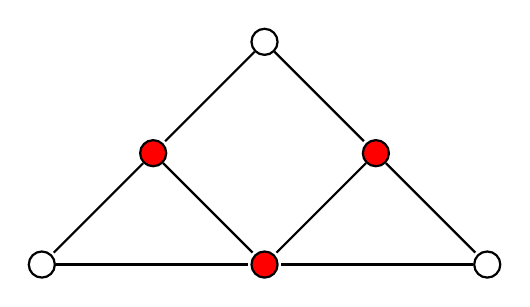
\begin{tikzpicture}[-,>=stealth,shorten >=1pt,auto,node distance=2cm,thick,main node/.style={scale=1,circle,draw,font=\sffamily\normalsize}]
            \node[main node] (1) []{};
            \node[main node] (2) [fill=red, below left of=1] {};
            \node[main node] (3) [fill=red, below right of=1] {};
            \node[main node] (4) [fill=red, below right of=2] {};
            \node[main node] (5) [below left of=2] {};
            \node[main node] (6) [below right of=3] {};

            \path[every node/.style={font=\sffamily\small}]
                (1) edge (2)
                (1) edge (3)
                (2) edge (4)
                (3) edge (4)
                (2) edge (5)
                (3) edge (6)
                (5) edge (4)
                (6) edge (4)
                ;
        \end{tikzpicture}

        \textit{The red nodes are the smallest possible vertex cover of the graph}
    \end{center}

    \begin{framedprob}{The Minimum Vertex Cover problem}
        Given an undirected graph $G$, find a vertex cover $X \subseteq V(G)$ with the fewest amount of nodes possible, meaning that:
        \[X = \argmin_{\substack{H \text{ vertex}\\ \text{cover of } G}} \rbk{\abs{H}}\]
    \end{framedprob}

    Like the two previous problems, we can easily formulate the Minimum Vertex Cover problem as a 0-1 integer program:
    \begin{itemize}
        \item For every node $v \in V(G)$, we define the variabile $x_v$.
        \item For every edge $(i,j) \in E(G)$ we add the constraint $x_i + x_j \geq 1$. This constraint enforces that at least one between $x_i$ and $x_j$ has to be set to 1.
    \end{itemize}

    We get that:
    \[\begin{array}{ccc}
        \qquad\qquad\quad
        & \min \; \sum\limits_{i = 1}^n x_i \\\\
        & x_i + x_j \geq 1 & \forall (i,j) \in E(G) \\
        & x \in \{0,1\}^n
    \end{array}\]

    By the very own definition of the integer program, we notice that the Minimum Vertex Cover problem is actually the \textbf{complementary of the Maximum Independent Set problem}, a particular case of the Maximum-weight Independent Set problem where all the weights are set to 1. This fact is well known in graph theory and it's stated through the following more general result which directly derives from our observation:
    \begin{framedthm}{}
        Given an undirected graph $G$, a subset $X \subseteq V(G)$ is a \textbf{vertex cover} if and only if $V(G) - X$ is an \textbf{independent set}.
    \end{framedthm}

    The Minimum Vertex Cover problem is also highly related to other graph theory problems. Through the properties of linear programming we can show such results with ease. For example, consider the \textbf{dual} of the Minimum Vertex Cover problem: by transposing the constraint matrix we get constraints on the number of edges available for each node. 
    \[\begin{array}{ccc}
        \qquad\qquad\quad
        & \max \; \sum\limits_{i = 1}^m y_i \\\\
        & \sum\limits_{e \in \delta(v)} x_e \leq 1 & \forall v \in V(G) \\
        & y \in \{0,1\}^m
    \end{array}\]

    A good eye will notice that this dual program corresponds to the \textbf{Maximum Matching problem for bipartite graphs}, a particular case of the Maximum-weight Perfect Matching problem where all the weights are set to 1 and the matchings aren't required to be perfect.
    
    Since both the primal and the dual have a feasible solution, by the \textbf{strong duality theorem} we know that they share the same optimum, giving us the following theorem "for free".

    \begin{framedthm}{Kőnig's theorem}
        Given an undirected bipartite graph $G$, the cardinality of the minimal vertex cover $X \subseteq V(G)$ is \textbf{equal} to the cardinality of the maximal matching $M \subseteq E(G)$.
    \end{framedthm}

    \newpage

    \section{Solved exercises}

    \begin{framedprob}{}
        Let $G$ be a bipartite graph defined by the independent sets $A, B$ such that $\abs{A} = \abs{B}$. Give a linear programming formulation to find the maximum cardinality matching in $G$, that is a matching $M$ in $G$ which maximizes $\abs{M}$. Prove that the formulation gives a correct optimal solution.
    \end{framedprob}

    \textit{Solution:}

    By definition, a matching on $G$ is a subset $M \subseteq E(G)$ such that $\nexists v \in V(G)$ for which $(v,x), (v,y) \in E(G)$, meaning that for every node of $G$ there is at most one edge incident to it. For each edge $e \in E(G)$, we define the variable $x_e$. Moreover, for each node $v$ we define $\delta(v) = \{e \in E(G) \mid e = (v,u), u \in V(G)\}$, i.e. the set of edges that are incident to $v$.
    
    Consider the following integer program:
    \[\begin{array}{ccc}
        \qquad\qquad\quad
        & \max \; \sum\limits_{e \in E(G)} x_e \\\\
        & \sum\limits_{e \in \delta(v)} x_e \leq 1 & \forall v \in V(G) \\
        & x \in \{0,1\}^m
    \end{array}\]

    For each feasible solution $x$, let $M_x = \{e \in E(G) \mid x_e > 0\}$, that being the matching represented by $x$. By this formulation, it's easy to see that any optimal solution of the integer program corresponds to a maximal matching of $G$.

    Consider now the LP relaxation of this integer program.
    \[\begin{array}{ccc}
        \qquad\qquad\quad
        & \max \; \sum\limits_{e \in E(G)} x_e \\\\
        & \sum\limits_{e \in \delta(v)} x_e \leq 1 & \forall v \in V(G) \\
        & 0 \leq x \leq 1 \\
        & x \in \R^m
    \end{array}\]

    In this relaxed form, rational values are allowed, meaning that $M_x$ correctly describes a matching only if $x$ is an integral solution. Since $G$ is a bipartite graph defined by two independent sets of the same cardinality, the vertices of the polyhedron $P$ described by this linear program are all integral. In particular, since the program is bounded, one of these vertices will correspond to an optimal solution. Hence, by applying the Simplex method, we can find an optimal integral BFS corresponding to a maximal matching.
    
\end{document}